\def\COMPLETE{}
\documentclass[letterpaper,12pt,titlepage,oneside,final]{book}
 
\newcommand{\package}[1]{\textbf{#1}} 
\newcommand{\cmmd}[1]{\textbackslash\texttt{#1}} 
\newcommand{\href}[1]{#1} 
\usepackage{ifthen}
\newboolean{PrintVersion}
\setboolean{PrintVersion}{false} 

\usepackage{amsmath,amssymb,amstext,amsthm,mathtools} 
\usepackage[pdftex]{graphicx} 
\usepackage{thm-restate}

\usepackage[pdftex,pagebackref=false]{hyperref} 
\usepackage[boxruled]{algorithm2e}

\usepackage{chngcntr}
\usepackage[toc,page]{appendix}
\usepackage[inline]{enumitem}
\usepackage{bbm}

\usepackage[labelformat=simple]{subcaption}
\usepackage[export]{adjustbox}

\usepackage{tikz}
\usetikzlibrary{shapes, calc, arrows, through, intersections, decorations.pathreplacing, patterns}

\newcommand{\mc}{\mathcal}
\newcommand{\mb}{\mathbf}
\newcommand{\tr}{\text{Tr}}
\newcommand{\diag}{\text{diag}}
\DeclareMathOperator*{\argmin}{arg\,min}
\DeclareMathOperator*{\argmax}{arg\,max}
\DeclareMathOperator{\vcdim}{VC-Dim}
\DeclareMathOperator{\vol}{vol}

\renewcommand\labelitemi{$\bullet$}
\renewcommand{\labelitemii}{$\star$}
\renewcommand\thesubfigure{(\alph{subfigure})}

\newtheorem{theorem}{Theorem}
\newtheorem{lemma}[theorem]{Lemma}
\newtheorem{definition}[theorem]{Definition}
\newtheorem{proposition}[theorem]{Proposition}
\newtheorem{corollary}[theorem]{Corollary}
\newtheorem{thrm}[theorem]{Theorem}
\newtheorem{lem}[theorem]{Lemma}
\newtheorem{smallLemma}{Claim}

\newcommand\numberthis{\addtocounter{equation}{1}\tag{\theequation}}
\let\oldnl\nl
\newcommand{\nonl}{\renewcommand{\nl}{\let\nl\oldnl}}
\newcommand{\multlinecomment}[1]{\directlua{-- #1}}

\hypersetup{
    plainpages=false,       
    unicode=false,          
    pdftoolbar=true,        
    pdfmenubar=true,        
    pdffitwindow=false,     
    pdfstartview={FitH},    
    pdftitle={Shrinu\ Kushagra\ Thesis},    
    pdfauthor={Shrinu Kushagra}, 
    pdfsubject={Clustering},  
%    pdfkeywords={keyword1} {key2} {key3}, % list of keywords, and uncomment this line if desired
    pdfnewwindow=true,      % links in new window
    colorlinks=true,        % false: boxed links; true: colored links
    linkcolor=blue,         % color of internal links
    citecolor=green,        % color of links to bibliography
    filecolor=magenta,      % color of file links
    urlcolor=cyan           % color of external links
}
\ifthenelse{\boolean{PrintVersion}}{   % for improved print quality, change some hyperref options
\hypersetup{	% override some previously defined hyperref options
%    colorlinks,%
    citecolor=black,%
    filecolor=black,%
    linkcolor=black,%
    urlcolor=black}
}{} % end of ifthenelse (no else)

\usepackage[automake,toc,abbreviations]{glossaries-extra} %
\setlength{\marginparwidth}{0pt}
\setlength{\marginparsep}{0pt} 
\setlength{\evensidemargin}{0.125in}
\setlength{\oddsidemargin}{0.125in}
\setlength{\textwidth}{6.375in} 
\raggedbottom

\setlength{\parskip}{\medskipamount}

\renewcommand{\baselinestretch}{1} % this is the default line space setting

\let\origdoublepage\cleardoublepage
\newcommand{\clearemptydoublepage}{%
  \clearpage{\pagestyle{empty}\origdoublepage}}
\let\cleardoublepage\clearemptydoublepage

\newglossaryentry{computer}
{
name=computer,
description={A programmable machine that receives input data,
               stores and manipulates the data, and provides
               formatted output}
}

% Nomenclature glossary entries -- New definitions, or unusual terminology
\newglossary*{nomenclature}{Nomenclature}
\newglossaryentry{dingledorf}
{
type=nomenclature,
name=dingledorf,
description={A person of supposed average intelligence who makes incredibly brainless misjudgments}
}

\newabbreviation{aaaaz}{AAAAZ}{American Association of Amature Astronomers and Zoologists}

% List of Symbols
\newglossary*{symbols}{List of Symbols}
\newglossaryentry{rvec}
{
name={$\mathbf{v}$},
sort={label},
type=symbols,
description={Random vector: a location in n-dimensional Cartesian space, where each dimensional component is determined by a random process}
}

\makeglossaries

\AtBeginEnvironment{subappendices}{%
\chapter*{Appendices}
\addcontentsline{toc}{chapter}{\hspace{0.09in}Appendices}
\counterwithin{figure}{section}
\counterwithin{table}{section}
}

\begin{document}
\ifdefined\COMPLETE
\else
\documentclass[letterpaper,12pt,titlepage,oneside,final]{book}

\usepackage{ifthen}
\newboolean{PrintVersion}
\setboolean{PrintVersion}{false} 

\usepackage[pdftex]{graphicx} 
\usepackage[pdftex,pagebackref=false]{hyperref} 

\hypersetup{
    plainpages=false,       
    unicode=false,          
    pdftoolbar=true,        
    pdfmenubar=true,        
    pdffitwindow=false,     
    pdfstartview={FitH},    
    pdftitle={Shrinu\ Kushagra\ Thesis},    
    pdfauthor={Shrinu Kushagra}, 
    pdfsubject={Clustering},  
%    pdfkeywords={keyword1} {key2} {key3}, % list of keywords, and uncomment this line if desired
    pdfnewwindow=true,      % links in new window
    colorlinks=true,        % false: boxed links; true: colored links
    linkcolor=blue,         % color of internal links
    citecolor=green,        % color of links to bibliography
    filecolor=magenta,      % color of file links
    urlcolor=cyan           % color of external links
}
\ifthenelse{\boolean{PrintVersion}}{   % for improved print quality, change some hyperref options
\hypersetup{	% override some previously defined hyperref options
%    colorlinks,%
    citecolor=black,%
    filecolor=black,%
    linkcolor=black,%
    urlcolor=black}
}{} % end of ifthenelse (no else)

\setlength{\marginparwidth}{0pt}
\setlength{\marginparsep}{0pt} 
\setlength{\evensidemargin}{0.125in}
\setlength{\oddsidemargin}{0.125in}
\setlength{\textwidth}{6.375in} 
\raggedbottom

\setlength{\parskip}{\medskipamount}

\renewcommand{\baselinestretch}{1} % this is the default line space setting

\let\origdoublepage\cleardoublepage
\newcommand{\clearemptydoublepage}{%
  \clearpage{\pagestyle{empty}\origdoublepage}}
\let\cleardoublepage\clearemptydoublepage


\begin{document}
\fi
\pagestyle{empty}
\pagenumbering{roman}

\begin{titlepage}
        \begin{center}
        \vspace*{1.0cm}

        \Huge
        {\bf Theoretical foundations for efficient clustering}

        \vspace*{1.0cm}

        \normalsize
        by \\

        \vspace*{1.0cm}

        \Large
        Shrinu Kushagra \\

        \vspace*{3.0cm}

        \normalsize
        A thesis \\
        presented to the University of Waterloo \\ 
        in fulfillment of the \\
        thesis requirement for the degree of \\
        Doctor of Philosophy \\
        in \\
        Computer Science \\

        \vspace*{2.0cm}

        Waterloo, Ontario, Canada, 2019 \\

        \vspace*{1.0cm}

        \copyright\ Shrinu Kushagra 2019 \\
        \end{center}
\end{titlepage}

\pagestyle{plain}
\setcounter{page}{2}

\cleardoublepage
\begin{center}\textbf{Examining Committee Membership}\end{center}
  \noindent
The following served on the Examining Committee for this thesis. The decision of the Examining Committee is by majority vote.
  \bigskip
  
  \noindent
\begin{tabbing}
Internal-External Member: \=  \kill % using longest text to define tab length
External Examiner: \>  Sanjoy Dasgupta \\ 
\> Professor, Computer Science and Engineering\\ \> University of California, San Diego \\
\end{tabbing} 
  \bigskip
  
  \noindent
\begin{tabbing}
Internal-External Member: \=  \kill % using longest text to define tab length
Supervisor(s): \> Shai Ben-David \\
\> Professor, Dept. of Computer Science, University of Waterloo \\
\end{tabbing}
  \bigskip
  
  \noindent
  \begin{tabbing}
Internal-External Member: \=  \kill % using longest text to define tab length
Internal Member: \> Yaoliang Yu \\
\> Assistant Professor, Dept. of Computer Science\\
\> University of Waterloo \\
\end{tabbing}
  \bigskip
  
  \noindent
\begin{tabbing}
Internal-External Member: \=  \kill % using longest text to define tab length
Internal-External Member: \> Chaitanya Swamy \\
\> Professor, Dept. of Combinatorics \& Optimization\\ \>University of Waterloo \\
\end{tabbing}
  \bigskip
  
  \noindent
\begin{tabbing}
Internal-External Member: \=  \kill % using longest text to define tab length
Other Member(s): \> Eric Blais \\
\> Assistant Professor, Dept. of Computer Science\\
\> University of Waterloo \\
\end{tabbing}

\cleardoublepage

\begin{center}\textbf{Statement of Contributions}\end{center}
  \noindent
This thesis consists of material all of which I authored or co-authored. Chapter \ref{chapter:activeClustering} is based on a joint work with Hassan Ashtiani and Shai Ben-David \cite{ashtiani2016clustering}. The first part of Chapter \ref{chapter:deduplication} (the framework of promise correlation clustering) is based on a joint work with Ihab Ilyas and Shai Ben-David \cite{kushagra2019semisupervised}. The experimental and hashing based algorithm in this chapter is based on the joint work with Hemant Saxena, Ihab Ilyas and Shai Ben-David \cite{kushagra2019asemisupervised}. Chapter \ref{chapter:optimizationClustering} is based on a joint work with Yaoliang Yu and Shai Ben-David \cite{kushagra2017provably}. Chapter \ref{chapter:clusteringNoise} is based on a joint work with Samira Samadi and Shai Ben-David \cite{kushagra2016finding}

  \bigskip
  
  \noindent
I understand that my thesis may be made electronically available to the public.

\cleardoublepage

\begin{center}\textbf{Abstract}\end{center}
Clustering aims to group together data instances which are similar while simultaneously separating the dissimilar instances. The task of clustering is challenging due to many factors. The most well-studied is the high computational cost. The clustering task can be viewed as an optimization problem where the goal is to minimize a certain cost function (like $k$-means cost or $k$-median cost). Not only are the minimization problems NP-Hard but often also NP-Hard to approximate (within a constant factor). There are two other major issues in clustering, namely \emph{under-specificity} and \emph{noise-robustness}. The focus of this thesis is tackling these two issues while simultaneously ensuring low computational cost. 

Clustering is an under-specified task. The same dataset may need to be clustered in different ways depending upon the intended application. Different solution requirements need different approaches. In such situations, domain knowledge is needed to better define the clustering problem. We incorporate this by allowing the clustering algorithm to interact with an oracle by asking whether two points belong to the same or different cluster. In a preliminary work, we show that access to a small number of same-cluster queries makes an otherwise NP-Hard $k$-means clustering problem computationally tractable. Next, we consider the problem of clustering for data de-duplication; detecting records which correspond to the same physical entity in a database. We propose a correlation clustering like framework to model such record de-duplication problems. We show that access to a small number of same-cluster queries can help us solve the `restricted' version of correlation clustering. Rather surprisingly, more relaxed versions of correlation clustering \footnote{We refer to it as promise correlation clustering.} are intractable even when allowed to make a `large' number of same-cluster queries. 

Next, we explore the issue of noise-robustness of clustering algorithms. Many real-world datasets, have on top of cohesive subsets, a significant amount of points which are `unstructured'. The addition of these \textit{noisy} points makes it difficult to detect the structure of the remaining points. In the first line of work, we develop a generic procedure that can transform objective-based clustering algorithms into one that is robust to outliers (as long the number of such points is not `too large'). In particular, we develop efficient noise-robust versions of two common clustering algorithms and prove robustness guarantees for them. In the second line of work, we define noise as not having significantly large dense subsets. We provide computationally efficient clustering algorithms that capture all meaningful clusterings of the dataset; where the clusters are cohesive (defined formally by notions of clusterability) and where the noise satisfies the gray background assumption. We complement our results by showing that when either the notions
of structure or the noise requirements are relaxed, no such results are
possible.

   

\cleardoublepage

\begin{center}\textbf{Acknowledgements}\end{center}

I would like to thank all the little people who made this thesis possible.
\cleardoublepage

\begin{center}\textbf{Dedication}\end{center}

\begin{center}{In the loving memory of Shreya.}\end{center}
\cleardoublepage

\renewcommand\contentsname{Table of Contents}
\tableofcontents
\cleardoublepage
\phantomsection    % allows hyperref to link to the correct page

% L I S T   O F   T A B L E S
% ---------------------------
\addcontentsline{toc}{chapter}{List of Tables}
\listoftables
\cleardoublepage
\phantomsection		% allows hyperref to link to the correct page

% L I S T   O F   F I G U R E S
% -----------------------------
\addcontentsline{toc}{chapter}{List of Figures}
\listoffigures
\cleardoublepage
\phantomsection		% allows hyperref to link to the correct page

% GLOSSARIES (Lists of definitions, abbreviations, symbols, etc. provided by the glossaries-extra package)
% -----------------------------
%\printglossaries
%\cleardoublepage
\phantomsection		% allows hyperref to link to the correct page

% Change page numbering back to Arabic numerals
\pagenumbering{arabic}

\ifdefined\COMPLETE
\else
\end{document}
\fi 

\chapter{Introduction}
\label{chapter:introduction}
\def\ACCOMPLETE{}
\ifdefined\COMPLETE
\else
\documentclass[12pt]{article}
\usepackage{amsmath,amssymb,amstext,amsthm} 
\usepackage[boxruled]{algorithm2e}
\usepackage{tikz}
\usepackage[inline]{enumitem}

\newcommand{\mc}{\mathcal}
\newcommand{\mb}{\mathbf}
\DeclareMathOperator*{\argmin}{arg\,min}
\DeclareMathOperator*{\argmax}{arg\,max}
\DeclareMathOperator{\vcdim}{VC-Dim}

\newtheorem{theorem}{Theorem}
\newtheorem{lemma}[theorem]{Lemma}
\newtheorem{definition}[theorem]{Definition}
\newtheorem{proposition}[theorem]{Proposition}
\newtheorem{corollary}[theorem]{Corollary}

\usetikzlibrary{shapes, calc, arrows, through, intersections, decorations.pathreplacing, patterns}

\begin{document}
\fi

Clustering is a term used to describe a wide variety of unsupervised learning algorithms. One popular definition of clustering is that it attempts to partition a given dataset into subsets (or {\em clusters}) such that similar points share the same cluster and dissimilar points are separated into different clusters. Clustering is a very challenging task and in this thesis we examine three such challenges.

The first challenge that we address is computational complexity. This is one of the most well-studied challenges of clustering. Clustering is commonly posed as an optimization problem where the goal is to minimize a certain cost function. For many common cost functions such as $k$-means or $k$-median or $k$-center it is known that the optimization problem is NP-hard \cite{dasgupta2008hardness}, \cite{megiddo1984complexity}.

The second challenge that we examine is the issue of {\em under-specificity}. The basic definition of clustering requires an algorithm to partition the dataset into coherent subsets which are `well-separated'. On a closer look, we see that this definition is problematic. Consider a set of (say $n$) points on a straight line where each pair of adjacent points have a small distance (say $\alpha$) between them. If we impose the requirement that each pair of similar points should share a cluster then all the points would end up in a single cluster. This would violate the second requirement as dissimilar points would also share the same cluster. Similarly, if we require that all the dissimilar instances be separated then we would end up separating similar pairs of points as well. This example is shown in Fig. \ref{fig:conflictingReq}

\begin{figure}

\includegraphics[trim={100 650 30 120},clip,width=\textwidth]{figures/conflictingReq.pdf}
\caption{An example of $n$ points on the real line separated by a small distance $\alpha$. This figure highlights that it is not always possible to satisfy the two requirements from clustering algorithms.}
\label{fig:conflictingReq}
\end{figure}

Hence, different algorithms `focus more' on different aspects of the clustering definition. For example, single-linkage tries to put similar points in the same cluster. However, it may end up having dissimilar points in the same cluster as well. On the other hand, the Lloyd's algorithm tries to separate dis-similar points but may end up separating similar points as well. The basic definition of clustering does not have enough information to resolve this conflict. Thus, we say that the clustering problem is under-specified. The fundamental question that we ask here is that `how do we prefer one clustering algorithm over another?'

We address the problem of under-specificity by incorporating domain knowledge into the clustering problem. The clustering algorithm is allowed to interact with an oracle (or an expert) by asking whether two points should belong to the same or different clusters. The oracle replies either `yes' or `no' to the \textit{same-cluster} query depending upon whether the two points belong to the same or different clusters. In this case, the goal of the clustering algorithm is to recover the clustering which the oracle has in its `mind'.

In the first part of the thesis we simultaneously address the challenges of under-specificity and computational cost. We study the \textit{computational} and \textit{query} complexity of various clustering problems in this framework. Consider the following simple observation. Given any clustering instance, if the algorithm is allowed to make $n^2$ (where $n$ is the size of the dataset) queries to the same-cluster oracle then recovering the true or target clustering is trivial. In this dissertation, one of the important questions that we examine is the following. {Is it possible to efficiently solve (in polyniomial time) an otherwise intractable clustering problem while making a `small' number of same-cluster queries to the oracle?}  

Now, we discuss the third challenge; namely the issue of \textit{noise-robustness} of clustering algorithms. The basic definition of clustering says that the goal is to partition a dataset into clusters such that similar points share a cluster while dissimlar points are separated into different clusters. This definition makes sense when the given dataset has a cohesive structure. That is, the dataset can be partitioned into groups or clusters which have some inter-cluster separation. However, real-world datasets, on top of this structure, have a significant subset of points which are unstructured. The addition of these \textit{noisy} points makes it difficult for the clustering algorithm to detect the structure of remaining points. The precise definition of `unstructuredness' or noisy points varies depending upon the structure that the clustering algorithm is trying to detect. In this dissertation, we consider two definitions of noise and develop efficient noise-robust clustering algorithms in each case.

We address all the challenges of clustering under a formal framework. The goal is to have a framework which can be mathematically analyzed and is also relevant to practitioners. Obviously, the exact framework varies depending upon the clustering problem we are considering. To analyze these issues in a formal framework, we will be mostly relying on mathematical theorems and proofs. But in some cases (where applicable), we have also complemented our results with experiments and simulations. 

\section{Our Contributions} 
As we alluded to before, our contributions can be divided into two categories. One is dealing with under-specificity and the second related to noise robustness of clustering algorithms. In this next sub-sections, we go into more details of each of these and outline our  objectives and contributions made. 

\subsection{Under-specificity}
The first main contribution is to develop a formal framework to incorporate domain knowledge into the clustering problem. We introduce a semi-supervised clustering framework. The learner is allowed to interact with a domain expert (or an oracle) by asking whether two data instances belong to the same  or different cluster (same-cluster query). The oracle has a target clustering in its mind and responds by answering either `yes' or `no' (depending upon whether the two points belong to the same or different clusters according to the target clustering). We assume that the oracle is perfect and has complete knowledge of the ground truth clustering. Hence, given any pair of points it always gives the correct response. We consider two clustering problems under this framework.

\subsubsection*{Clustering with advice ($k$-means)}
We consider a setting where the oracle conforms to a center-based clustering with a notion of margin. That is, the target clustering has the following property.  Every cluster-center is `more' closer ($\gamma$-times closer) to points in its own cluster than to points in a different cluster. Larger values of $\gamma$ imply greater separation between different clusters. 

Under this framework, we study the query and computational complexity of recovering the target clustering. We provide an algorithm which runs in $O\big(kn\log n)$ time and makes $O\big(k\log n + k^2 \log k)$ same-cluster queries to the oracle and succeeds in recovering the oracle's clustering with high probability. Here $n$ is the size of the dataset and $k$ is the number of clusters.

We also consider the case when the oracle conforms to the optimal $k$-means clustering under $\gamma$-margin. Then, our query-based algorithm can find the optimal solution in polynomial time. Interestingly, we prove that even when the optimal $k$-means clustering satisfies margin conditions, without queries, finding that solution is NP-hard. Thus having access to relatively few oracle queries can allow efficient solutions to otherwise intractable problems.

\subsubsection*{Correlation clustering with advice}
We consider the problem of correlation clustering under the semi-supervised clustering framework. Correlation clustering is very useful for modelling the record de-duplication problem; the task of detecting multiple records that correspond to the same real-world entity in a database. Here the goal is to put records corresponding to the same physical entity in the same cluster and putting records corresponding to different physical entities into different clusters.

Formally, given a complete graph $G$ with the edges labelled $0$ and $1$, the goal of correlation clustering is to find a clustering that minimizes the number of $0$ edges within a cluster plus the number of $1$ edges across different clusters. In other words, the goal is to find a clustering which minimizes the \textit{correlation loss} w.r.t the graph $G$. \\

\noindent\textbf{\small Promise correlation clustering}\\
The optimal clustering $C^*$ can also be viewed as a complete graph $G^*$ (unknown to the clustering algorithm) with edges corresponding to points in the same cluster being labelled $1$ and other edges being labelled $0$. If it is known that the edge difference between $G$ and $G^*$ is zero, then finding $C^*$ is easy (find the connected components of $G$). We consider a variant of this problem where it is promised that the edge difference between $G$ and the unknown $G^*$ is ``small". The goal is to find the clustering which minimizes the correlation loss w.r.t $G$.

We now wish to analyze the computational and query complexity of the promise correlation clustering (PCC) problem. We prove that the promise version is still NP-hard. Rather surprisingly, we further prove that even with access to a same-cluster oracle, the promise version is intractable as long as the number queries to the oracle is $o(n)$ (the proof assumes the Exponential Time Hypothesis; $n$ is the number of vertices). \\

\noindent\textbf{\small Restricted correlation clustering}\\
Given these negative results, we consider a restricted version of correlation clustering. First observe that in the standard version, the goal is to find a clustering over the class of all possible clusterings of the dataset. Here, we restrict ourselves to a given class $\mc F$ of clusterings. Another difference is that we want to minimize the correlation loss w.r.t the unknown target clustering $C^*$ rather than a graph $G$. 

We now wish to analyze the query and computational complexity of this problem. We offer an algorithmic approach (using same-cluster queries) and prove that the query complexity is upper bounded by a term that depends only on the $\vcdim(\mc F)$ and is independent of the dataset size. We also provide computationally efficient algorithms for a few common classes of clusterings. 
 
\subsection{Noise-robustness}
We now describe our framework to address the issue of noise in clustering algorithms. We are given a dataset $X$ which is made up of two parts. The first is the structured or clusterable component $S$. Mathematically, this is captured by introducing notions of `clusterability of data'. Intuitively, these notions say that the set $S$ is composed of $k$ different clusters and the clusters are `well-separated' from each other. In this thesis, we consider two such notions, center-proximity and center-separation. Each of them formalize the idea of well-separatedness in a different way. The second component of the dataset is the noisy or unstructured part $N$. The clustering algorithm receives $X$ as its input. It does not have any knowledge about $S$ (or its substructure) or $N$. The goal is to partition $X$ into components so that the structure of $S$ is \textit{preserved}. Any algorithm which achieves this goal is said to be noise-robust. 

\subsubsection*{Detecting cluster structure in the presence of sparse noise}
We consider the problem of detecting the structure of $S$ when the noisy part $N$ is sparse. That is, the only restriction about the noisy part of the data is that it does not create significantly large clusters. We introduce efficient algorithms that discover and cluster every subset $S$ of the data with the following property. $S$ has a meaningful structure (as captured by a notion of clusterability) and its complement is structureless or sparse. We say that our algorithm is robust to sparse noise. Notably, the success of our algorithms do not depend on any upper bound on the fraction of noisy data. We complement our results by showing that when either the notions of structure or the noise requirements are relaxed, no such results are possible.

\subsubsection*{Detecting cluster structure in the presence of outliers}
We propose a generic regularization-based method that transforms any center-based clustering objective into a noise-robust one. We use our procedure to obtain regularized versions of two common clustering algorithms based on the $k$-means objective function. We prove that these regularized algorithms are robust to outliers (under clusterability assumptions and mildness properties of the noisy points).

\section{Reading the thesis}
This dissertation is composed of two components. The first addresses the problem of under-specificity in clustering and is covered in Chapters \ref{chapter:activeClustering} and \ref{chapter:deduplication}. The second part is about the issue of noise-robustness of clustering algorithms and is covered in Chapters \ref{chapter:clusteringNoise} and \ref{chapter:optimizationClustering}. The two parts are independent of one another and the reader can start with whichever one he/she is more interested in. 

We have ensured that each chapter is self-contained. Note that the thesis does not have a dedicated chapter on related work or on notation/preliminaries. Rather these are included in the relevant chapters. Some of the missing proofs can be found in appendices at the end of the corresponding chapters.

\section{Technical background}
Some of the proofs in the thesis use the following classical results from learning theory literature. Readers who are unfamiliar with result can also refer to the standard texts on this subject, for example, \cite{shalev2014understanding}.
 

\subsection{Learning theory results}
\begin{theorem}[Vapnik and Chervonenkis \cite{vapnik2015uniform}]
\label{thm:vceapprox}
Let $X$ be a domain set and $D$ a probability distribution over $X$. Let $H$ be a class of subsets of $X$ of finite VC-dimension $d$. Let $\epsilon, \delta \in (0,1)$. Let $S \subseteq X$ be picked i.i.d according to $D$ of size $m$. If $m > \frac{c}{\epsilon^2}(d\log \frac{d}{\epsilon}+\log\frac{1}{\delta})$, then  with probability $1-\delta$ over the choice of $S$, we have that $\forall h \in H$
$$\bigg|\frac{|h\cap S|}{|S|} - P(h)\bigg| < \epsilon$$
\end{theorem}

\begin{theorem}[Fundamental theorem of learning \cite{blumer1989learnability}] 
\label{thm:uniformConvergence}
Here, we state the theorem as in the book \cite{shalev2014understanding}. Let $H$ be a class of functions $h:\mc X \rightarrow \{0, 1\}$ of finite VC-Dimension, that is $\vcdim(H) = d < \infty$. Let $D$ be a probability distribution over $X$ and $h^*$ be some unknown target function. Given $\epsilon, \delta \in (0, 1)$. Let $err_D$ be the $\{0, 1\}$-loss function $err: H \rightarrow [0, 1]$. That is $err_D(h) = \underset{x \in D}{\mb P}[h(x) \neq h^*(x)]$. Sample a set $S = \{(x_1, y_1), \ldots, (x_m, y_m)\}$ according to the distribution $D$. Define $err_S(h) = \sum_{i=1}^{m} \frac{\mb 1_{[h(x_i) \neq h^*(x_i)]}}{m}$. If $m \ge a\frac{d + \log (1/\delta)}{\epsilon^2}$, then with probability at least $1-\delta$ over the choice of $S$, we have that for all $h \in H$
$$|err_D(h) - err_S(h)| \le \epsilon$$
where $a$ is an absolute global constant. 
\end{theorem}

\subsection{Concentration inequalities}
Some of the proofs use the following concentration inequalities. 
\label{appendixsection:conIneq}
\begin{theorem}[Sum of geometric random variables \cite{brown2011wasted}]
\label{thm:geometricRV}
Let $X = X_1 + \ldots + X_n$ be $n$ geometrically distributed random variables such that $\mb E[X_i] = \mu$. Then 
$$\mb P[X > (1+\nu)n\mu] \le \exp\bigg(\frac{-\nu^2\mu n}{2(1+\nu)}\bigg)$$
\end{theorem}   

\begin{theorem}[Generalized Hoeffding's Inequality (e.g., \cite{ashtiani2015dimension})]
\label{thm:genHoeff}
Let $X_1, \ldots. X_n$ be i.i.d random vectors in some Hilbert space such that for all $i$, $\|X_i\|_2 \le R$ and $E[X_i] = \mu$. If $n > c\frac{\log(1/\delta)}{\epsilon^2}$, then with probability at least $1-\delta$, we have that
$$\Big\|\mu - \frac{1}{n}\sum X_i\Big\|_2^2 \le R^2\epsilon$$ 
\end{theorem}

\begin{theorem}[Multiplicative Chernoff bound \cite{mitzenmacher2005probability}]
\label{thm:chernoff}
Let\\ $X_1, \ldots, X_n$ be i.i.d random variables in $\{0, 1\}$ such that $\mu = E[X_i]$. Let $X = \frac{\sum X_i}{n}$. Then for any $0 < \epsilon < 1$
$$P\big[ \enspace X > (1+\epsilon) \mu\enspace\big] \enspace\le\enspace \exp\bigg(\frac{-\epsilon^2\mu n}{3}\bigg)$$
\end{theorem}

\begin{theorem}[Multiplicative Chernoff bound \cite{mitzenmacher2005probability}]
\label{thm:chernoff2}
Let\\ $X_1, \ldots, X_n$ be i.i.d random variables in $\{0, 1\}$ such that $\mu = E[X_i]$. Let $X = \frac{\sum X_i}{n}$. Then for any $0 < \epsilon < 1$
$$P\big[ \enspace X < (1-\epsilon) \mu\enspace\big] \enspace\le\enspace \exp\bigg(\frac{-\epsilon^2\mu n}{2}\bigg)$$
\end{theorem}


\ifdefined\COMPLETE
\else
\end{document}
\fi
































\chapter{Clustering with same-cluster queries}
\label{chapter:activeClustering}
\def\ACCOMPLETE{}
\ifdefined\COMPLETE
\else
\documentclass[12pt]{article}
\usepackage{amsmath,amssymb,amstext,amsthm} 
\usepackage[boxruled]{algorithm2e}
\usepackage{tikz}
\usepackage[inline]{enumitem}

\newcommand{\mc}{\mathcal}
\newcommand{\mb}{\mathbf}
\DeclareMathOperator*{\argmin}{arg\,min}
\DeclareMathOperator*{\argmax}{arg\,max}

\newtheorem{theorem}{Theorem}
\newtheorem{lemma}[theorem]{Lemma}
\newtheorem{definition}[theorem]{Definition}
\newtheorem{proposition}[theorem]{Proposition}
\newtheorem{corollary}[theorem]{Corollary}

\usetikzlibrary{shapes, calc, arrows, through, intersections, decorations.pathreplacing, patterns}

\begin{document}
\fi

Clustering is an under-specified task. Given a dataset, there is no unique or `correct' solution. The solution of choice varies with the intended application. In the absence of knowledge of the desired application, clustering problem is usually not well-defined. We need to incorporate domain expertise to better define the clustering problem. At the same time, performing clustering under many natural models of computation is computationally intractable. 

In this chapter, we take a new approach to alleviate these two issues in clustering. We first allow the clustering algorithm to be semi-supervised (through access to answers of natural queries). This makes the clustering problem better defined. We then ask the following question. \textit{Can semi-supervision help relax the computational burden of clustering?}

Aside from trial and error, one principled approach to supervision in clustering is through \textit{link/do-not-link} constraints \cite{basu2002semi,basu2004probabilistic, kulis2009semi}. In this case, besides the usual input, the clustering algorithm also receives a set of pairs which should always share the same cluster and a set of pairs which should always be separated into different clusters. Our approach combines the user-friendliness of link/do-not-link constraints with the advantages of interactiveness. We call it \textit{same-cluster} queries.  That is, the algorithm can interact with a domain expert (or an oracle) by asking whether two elements belong to the same cluster or not. The oracle responds by answering `yes' or `no' depending upon whether the two points share a cluster or are separated into different clusters. 

While same-cluster queries allow us to tackle the challenge of under-specificity, mitigating the computational intractability of clustering is equally important. Clustering is often posed as an optimization problem. Most common such formulations are NP-hard (for example, the $k$-means or $k$-median clustering problem). We can address this issue by exploiting the fact that natural data sets are usually `clusterable'. That is, they exhibit some nice properties and are likely to avoid worst-case scenarios. We introduce a novel notion of niceness of data (or a notion of clusterability) called $\gamma$-margin property. The notion says that each cluster is $\gamma$ times closer to the points in its own cluster than to points in different clusters. Thus, the larger the value of $\gamma$, the stronger the assumption becomes, which means that the clustering problem becomes easier. With respect to that $\gamma$ parameter, we get a sharp `phase transition' between $k$-means being NP hard and being optimally solvable in polynomial time\footnote{The exact value of such a threshold $\gamma$ depends on some finer details; whether $d$ is required to be Euclidean and whether the cluster centers must be members of $X$.}.

The general setting in this chapter is the following. Let $X$ be a set of elements that should be clustered and $d$ a distance metric over it. The oracle (e.g., a domain expert) has information about a target clustering $C^*$ in its mind. That target clustering satisfies some predefined clusterability condition. The clustering algorithm has access to $(X, d)$ and can also ask same-cluster queries about $C^*$. The goal of the algorithm is to efficiently recover the target clustering $C^*$ while make a `small' number of same-cluster queries to the oracle. We provide a polynomial time algorithm for clustering with queries, that succeeds (with high probability) under the assumption that the input satisfies the $\gamma$-margin condition for $\gamma > 1$. This algorithm makes $O\big(k^2\log k + k\log n)$ same-cluster queries to the oracle and runs in $O\big(kn\log n)$ time, where $k$ is the number of clusters and $n = |X|$.

We also consider the following special case. The target $C^*$ (in the oracle's mind) is the optimal solution of the $k$-means clustering problem and also satisfies the clusterability condition. In this case, the query-based algorithm succeeds with high probability as long as $\gamma >1$.  On the other hand, we show that without access to a same-cluster oracle, $k$-means clustering is NP-hard even when the optimal solution satisfies $\gamma$-margin property for $\gamma=\sqrt{3.4} \approx 1.84$ and $k=\Theta(n^\epsilon)$ (for any $\epsilon\in (0,1)$). This shows that access to a small number of same-cluster queries can provide an efficient algorithm for an otherwise NP-hard problem. This is an interesting trade-off between query complexity and computational complexity in the clustering domain. 


\section{Related Work}
This work combines two directions of research. The first is clustering under semi-supervision and the second is computational complexity of clustering. 

The most common framework to convey supervision in clustering is through a set of link/do-not-link constraints \cite{basu2002semi,basu2004probabilistic, kulis2009semi}. Here, the clustering algorithm is provided a list of pairs which should share the same cluster and a list of pairs which should be separated into different clusters. Here, the supervision is non-interactive. On the interactive side, Balcan et. al \cite{balcan2008clustering} introduced the notion of \textit{split/merge} queries. In their framework, the domain expert (or oracle) receives a clustering of the given dataset. Given a clustering, the oracle responds by suggesting either to merge two clusters or to split a cluster. For each query, the oracle should evaluate a clustering of the entire dataset. Another example of supervision is clustering was introduced by Ashtiani and Ben-David \cite{ashtiani2015representation}. Here, the oracle receives a small subset of the dataset and responds by outputting the `correct' clustering of that subset. Our approach combines the user-friendliness of link/do-not-link constraints (as opposed to requiring the oracle to answer queries about the whole data set or to cluster subsets of the data) with the advantages of interactiveness. 

The computational complexity of clustering is very well studied problem. Clustering is usually posed as an optimization problem where the goal is to minimize a given objective (or cost) function. $k$-means and $k$-median are two popular objective functions. However, many of the results are negative. For example, minimizing the $k$-means objective is NP-hard. Moreover, it is NP-Hard even for $k=2$ \cite{dasgupta2008hardness}, or even in a two-dimensional plane \cite{vattani2009hardness,mahajan2009planar}. Similarly, minimizing the $k$-median objective is also NP-Hard. Despite these negative results, clustering algorithms are routinely and successfully applied in practice. To explain this gap between theory and practice, notions of data niceness under which clustering becomes easy have been considered. The hypothesis is that real-world datasets are not worst-case and often have nice properties which makes clustering tractable. \cite{Ben-David15} has an extensive survey of such notions.

The notion of $\alpha$-center proximity introduced by Awasthi et. al \cite{awasthi2012center} is most related to our notion of margin (a comparison between the two can be found in Appendix \ref{appendix:gammaMrginVsAlphaCenter}). In the restricted scenario (i.e., when the centers of clusters are selected from the data set), their algorithm efficiently recovers the target clustering for $\alpha > 3$.  Balcan and Liang \cite{balcan2012clustering} provide a different algorithm and prove that recovery is possible for $\alpha > \sqrt{2} + 1$. Ben-David and Reyzin \cite{ben2014data} show that this problem is NP-Hard for $\alpha < 2$. Variants of these proofs for our $\gamma$-margin condition yield the feasibility of $k$-means clustering when the input satisfies the condition with $\gamma >2$ and NP hardness when $\gamma <2$.


\section{Problem Formulation}

Let $X$ be a subset of some Euclidean space, $\mb{R}^d$. A $k$-clustering of the set $X$ partitions it into $k$ disjoint subsets $\mc C = \{C_1, \ldots, C_k\}$ be a clustering  of $X$. We say $x_1 \overset{C}{\sim} x_2$ if $x_1$ and $x_2$ belong to the same cluster according to $C$. Also, $n := |X|$. We say that a clustering $C$ is \emph{center-based} if there exists centers $\mu = \{\mu_1, \ldots, \mu_k\} \subset \mb R^d$ such that $C$ corresponds to the Voronoi diagram over these centers. Namely, for every $x$ in $X$ and $i \leq k$,  $x\in C_i \Leftrightarrow i=\argmin_j d(x,\mu_j)$. 


Next, we introduce our data niceness property or our notion of clusterability of a data set.

\begin{definition}[$\gamma$-margin]
\label{defn:alphacp}
Let $X$ be set of points in a metric space $(M, d)$. Let $C = \{C_1, \ldots, C_k\}$ be a center-based clustering of $X$ induced by centers $\mu_1, \ldots, \mu_k \in M$. We say that $C$ satisfies the $\gamma$-margin property if the following holds. For all $i \in [k]$ and every $x \in C_i$ and $y \in X \setminus C_i$,

$$\gamma d(x, \mu_i) < d(y, \mu_i)$$
\end{definition}


We now introduce our notion of a same-cluster oracle and same-cluster queries. For a clustering $C^*=\{ C^*_1, \ldots C^*_k\}$, a $C^*$-oracle is a function ${\mc O} : X \rightarrow \{true, false\}$ that answers queries according to $C^*$. We can think of the oracle as a human or domain-expert that has knowledge about the desired clustering and can answer the clustering algorithm's queries. The clustering algorithm then tries to recover $C^*$ by querying $\mc O$.

\begin{definition}[Same-cluster Query]
Given a clustering instance $X$ and a $C^*$-oracle $\mc O$. A same-cluster query asks whether two instances $x_1$ and $x_2$ belong to the same cluster, i.e., 
$$\mc O(x_1, x_2) = \left\{
	\begin{array}{ll}
		\mbox{true }  & \mbox{if } x_1 \overset{C^*}{\sim} x_2   \\
		\mbox{false } & o.w. 
	\end{array}
\right. $$
\end{definition}

\section{Clustering using same-cluster queries}
\label{section:clusteringWithQuery}

In this section we provide an efficient algorithm for clustering with queries. The setting is the one described in the previous section. In particular, it is assumed that the oracle has a center-based clustering in his mind which satisfies the $\gamma$-margin property. The space is Euclidean and the center of each cluster is the center of mass of the instances in that cluster. The algorithm not only makes same-cluster queries, but also another type of query defined as below.% queiries to the oracle, but this can be translated to binary same-cluster queries 


\begin{definition}[Cluster-assignment Query]
A cluster-assignment query asks the cluster index that an instance $x$ belongs to. In other words ${\mc O_{C^*}}(x) = i$ if and only if $x \in C^*_i$.
\end{definition}

Note however that each cluster-assignment query can be replaced with $k$ same-cluster queries (see appendix \ref{appendix:diffQueryModels}). Therefore, we can express everything in terms of the more natural notion of same-cluster queries, and the use of cluster-assignment query is just to make the representation of the algorithm simpler.

Our algorithm works in two phases. In the first phase, it approximate the center of one of the clusters. It does this by asking cluster-assignment queries about a set of randomly (uniformly) selected point, until it has a sufficient number of points from at least one cluster (say $C_p$). It uses the mean of these points $\mu_p^\prime$ as an approximation of the true cluster center $\mu_p$. 

In the second phase, the algorithm recovers all of the instances belonging to $C_p$. In order to do that, it first sorts all of the instances based on their distance to $\mu_p^\prime$. The margin assumption ensures that all of the points in $C_p$ lie inside a sphere centered at $\mu_p^\prime$ (which does not include points from any other cluster). It then tries to find the radius of this sphere by doing binary search using same-cluster queries. After that, the elements in $C_p$ will be located and can be removed from the data set. The algorithm repeats this process $k$ times to recover all of the clusters. The details of our approach is in Algorithm \ref{alg:steinerQueryPositive}. Note that $\beta$ is a small constant\footnote{It corresponds to the constant appeared in generalized Hoeffding inequality bound, discussed in Theorem \ref{thm:genHoeff} in appendix \ref{appendixsection:conIneq} }. 

\RestyleAlgo{boxruled}
\SetAlgoNoLine
\begin{algorithm}[!th]
 \caption{Algorithm for $\gamma(> 1)$-margin instances with queries}
 \label{alg:steinerQueryPositive}
 \KwIn{Clustering instance $X$, a $C^*$-oracle $\mc O$, the number of clusters $k$ and a parameter $\delta \in (0, 1)$}
 \KwOut{A clustering $C$ of the set $X$}

 \vspace{0.5em} $C = \{\}$, $S = X$ and $\eta = \beta \frac{\log k + \log(1/\delta)}{(\gamma-1)^4}$\\
 \While{$S \neq \phi$}{
 	\vspace{0.5em}\textbf{Phase 1}\\
 	Let $l = k \eta + 1$\\
	Draw $l$ points from $S$ uniformly at random\\
	Let $S_t = \{x \in S : {\mc O}(x)= t\}.$ where the oracle answers cluster-assignment queries about the members of $S$\\
    $p = \argmax_t |S_t|$ and $\mu_p' := \frac{1}{|S_p|}\sum_{x \in S_p} x$.\\

	\vspace{0.5em}\textbf{Phase 2}\\
    Sorts elements of $\{x: x\in S\}$ in increasing order of $d(x, \mu_p')$.\\    
    Binary search over $S$, to find $i$ such that $b_{i} \in C_p$ and $b_{i+1} \not\in C_p$. (This step involves making same-cluster queries to the oracle $\mc O$).\\ %We will later prove that $d(b_{idx}, c_p') = \max_{x \in C_p}d(x, c_p')$.
	$C_p' = \{x \in S: d(x, \mu_p') \le d(b_i, \mu_p')\}$.\\
	Delete $C_p'$ from $S$ and $C = C \cup \{C_p'\}$
 }
\end{algorithm}

Theorem \ref{thm:steinerQueryPositive} shows that if $\gamma > 1$ then our algorithm recovers the target clustering with high probability. Next, we give bounds on the time and query complexity of our algorithm. Theorem \ref{thm:steinerQueryPositiveComplexity} shows that our approach needs $O(k\log n + k^2\log k)$ queries and runs with time complexity $O(kn\log n)$.




\begin{lemma}
\label{lemma:hasGammaMargin}
Given a clustering instance $X \subseteq \mb R^d$. Let $C = \{C_1, \ldots, C_k\}$ be any center-based clustering of $X$ that satisfies the $\gamma$-margin property. Let $\mu_i$ be the set of centers corresponding to the centers of mass of $C_i$. Let $\mu_i'$ be such that $d(\mu_i, \mu_i') \le r(C_i)\epsilon$, where $r(C_i) = \max_{x\in C_i}d(x, \mu_i)$ . If $\gamma \ge 1 + 2\epsilon$ then 
$$\forall x \in C_i, \forall y \in {X} \setminus C_i \Rightarrow d(x, \mu_i') < d(y, \mu_i')$$
\end{lemma}

\begin{proof}
Fix any $x \in C_i$ and $y \in C_j$. $d(x, \mu_i') \le d(x, \mu_i)+d(\mu_i, \mu_i') \le r(C_i) (1+\epsilon)$. Similarly, $d(y, \mu_i') \ge d(y, \mu_i) - d(\mu_i, \mu_i') > (\gamma -\epsilon)r(C_i)$. Combining the two, we get that $d(x, \mu_i') < \frac{1+\epsilon}{\gamma-\epsilon}d(y, \mu_i')$. 
\end{proof}

\begin{lemma}
\label{lemma:phase1}
Let the framework be as in Lemma \ref{lemma:hasGammaMargin}. Let $S_p, C_p, \mu_p$, $\mu_p^\prime$ and $\eta$ be defined as in Algorithm \ref{alg:steinerQueryPositive}, and $\epsilon = \frac{\gamma - 1}{2}$. If $|S_p| > \eta$, then the probability that $d(\mu_p, \mu_p^\prime) > r(C_p)\epsilon$ is at most $\frac{\delta}{k}$.
\end{lemma}
\begin{proof}
Define a uniform distribution $U$ over $C_p$. Then $\mu_p$ and $\mu_p^\prime$ are the true and empirical mean of this distribution. Using a standard concentration inequality (Thm. \ref{thm:genHoeff} from Appendix \ref{appendixsection:conIneq}) shows that the empirical mean is close to the true mean, completing the proof. 

\end{proof}

\begin{theorem}
\label{thm:steinerQueryPositive}
Given a clustering instance $X \subseteq \mb R^d$. Let $C^* = \{C_1^*, \ldots, C_k^*\}$ be center-based clustering of $X$ that satisfies the $\gamma$-margin property. Given $\delta \in (0, 1)$ and $\gamma > 1$ and a $C^*$-oracle, with probability at least $1-\delta$, Algorithm \ref{alg:steinerQueryPositive} outputs $C^*$.
\end{theorem}

\begin{proof}
In the first phase of the algorithm we are making $l>k\eta$ cluster-assignment queries. Therefore, using the pigeonhole principle, we know that there exists cluster index $p$ such that $|S_p| > \eta$. Then Lemma \ref{lemma:phase1} implies that the algorithm chooses a center $\mu_p^\prime$ such that with probability at least $1-\frac{\delta}{k}$ we have $d(\mu_p, \mu_p^\prime) \le r(C_p)\epsilon$. By Lemma \ref{lemma:hasGammaMargin}, this would mean that $d(x, \mu_p^\prime) < d(y, \mu_p')$ for all $x \in C_p$ and $y \not\in C_p$. Hence, the radius $r_i$ found in the phase two of Alg. \ref{alg:steinerQueryPositive} is such that $r_{i} = \max\limits_{x \in C_p} d(x, \mu_p^\prime)$. This implies that $C_p^\prime$ (found in phase two) equals to $C_p$. Hence, with probability at least $1-\frac{\delta}{k}$ one iteration of the algorithm successfully finds all the points in a cluster $C_p$. Using union bound, we get that with probability at least $1-k\frac{\delta}{k} = 1-\delta$, the algorithm recovers the target clustering.
\end{proof}

\begin{theorem}
\label{thm:steinerQueryPositiveComplexity}
Let the framework be as in theorem \ref{thm:steinerQueryPositive}. Then Algorithm \ref{alg:steinerQueryPositive} 
\begin{itemize}[nolistsep,noitemsep]
\item Makes $O\big(k\log n + k^2\frac{\log k + \log (1/\delta)}{(\gamma - 1)^4}\big)$ same-cluster queries to the oracle $\mc O$.
\item Runs in $O\big(kn\log n + k^2\frac{\log k + \log (1/\delta)}{(\gamma - 1)^4}\big)$ time.
\end{itemize}
\end{theorem}

\begin{proof}
In each iteration (i) the first phase of the algorithm takes $O(\eta)$ time and makes $\eta+1$ cluster-assignment queries (ii) the second phase takes $O(n\log n)$ times and makes $O(\log n)$ same-cluster queries. Each cluster-assignment query can be replaced with $k$ same-cluster queries; therefore, each iteration runs in $O(k\eta + n\log n)$ and uses $O(k\eta + \log n)$ same-cluster queries. By replacing $\eta = \beta\frac{\log k + \log(1/\delta)}{(\gamma-1)^4}$ and noting that there are $k$ iterations, the proof will be complete.
\end{proof}

\section{Hardness of $k$-means with Margin}
\label{section:lowerBounds}

Finding $k$-means solution without the help of an oracle is generally computationally hard. In this section, we will show that solving Euclidean $k$-means remains hard even if we know that the optimal solution satisfies the $\gamma$-margin property for $\gamma=\sqrt{3.4}$. In particular, we show the hardness for the case of $k=\Theta(n^\epsilon)$ for any $\epsilon\in (0,1)$.

%This is a critical result for our purpose, because it shows that our niceness assumption (i.e., the $\gamma$-margin property) is not too strong, and the use of oracle is necessary.

In Section \ref{section:clusteringWithQuery}, we proposed a polynomial-time algorithm that could recover the target clustering using $O(k^2\log k +k\log n)$ queries, assuming that the clustering satisfies the $\gamma$-margin property for $\gamma>1$. Now assume that the oracle conforms to the optimal $k$-means clustering solution. In this case, for $1<\gamma\le \sqrt{3.4} \approx 1.84$, solving $k$-means clustering would be NP-hard without queries, while it becomes efficiently solvable with the help of an oracle \footnote{To be precise, note that the algorithm used for clustering with queries is probabilistic, while the lower bound that we provide is for deterministic algorithms. However, this implies a lower bound for randomized algorithms as well unless $BPP\neq P$}. 

Given a set of instances $\mc X \subset \mb R ^d$, the $k$-means clustering problem is to find a clustering $\mc C = \{C_1, \ldots, C_k\}$ which minimizes $f(\mc C) = \sum\limits_{C_i} \min\limits_{\mu_i\in {\mb R}^d}\sum\limits_{x\in C_i} \|x - \mu_i \|_2^2$. The decision version of $k$-means is, given some value $L$, is there a clustering $\mc C$ with cost $\le L$? The following theorem is the main result of this section. 

\begin{theorem}
\label{thm:gammaLower}
Finding the optimal solution to Euclidean $k$-means objective function is NP-hard when $k=\Theta(n^\epsilon)$ for any $\epsilon \in (0,1)$, even when the optimal solution satisfies the $\gamma$-margin property for $\gamma = \sqrt{3.4}$.
\end{theorem}

This results extends the hardness result of \cite{ben2014data} to the case of Euclidean 
metric, rather than arbitrary one, and to the $\gamma$-margin condition (instead of the $\alpha$-center proximity there). In the next sections, we provide an outline of the proof. Some of the missing details can be found in the appendix (\ref{appendix:lowerBoundProof}).

\subsection{Overview of the proof}

Our method to prove Thm. \ref{thm:gammaLower} is based on the approach employed by \cite{vattani2009hardness}. However, the original construction proposed in \cite{vattani2009hardness} does not satisfy the $\gamma$-margin property. Therefore, we have to modify the proof by setting up the parameters of the construction more carefully. 

To prove the theorem, we will provide a reduction from the problem of Exact Cover by 3-Sets (\textsc{X3C}) which is NP-Complete \cite{garey2002computers}, to the decision version of $k$-means.
%(which given a real value $L$, asks whether a clustering with cost $\le L$ exists).

\begin{definition}[\textsc{X3C}]
Given a set $U$ containing exactly $3m$ elements and a collection $\mc S = \{S_1, \ldots, S_l\}$ of subsets of $U$ such that each $S_i$ contains exactly three elements, does there exist $m$ elements in $\mc S$ such that their union is $U$? 
\end{definition}

We will show how to translate each instance of X3C, $(U,\mc S)$, to an instance of $k$-means clustering in the Euclidean plane, $X$. In particular, $X$ has a grid-like structure consisting of $l$ rows (one for each $S_i$) and roughly $6m$ columns (corresponding to $U$) which are embedded in the Euclidean plane. The special geometry of the embedding makes sure that any low-cost $k$-means clustering of the points (where $k$ is roughly $6ml$) exhibits a certain structure. In particular, any low-cost $k$-means clustering could cluster each row in only two ways; One of these corresponds to $S_i$ being included in the cover, while the other means it should be excluded. We will then show that $U$ has a cover of size $m$ if and only if $X$ has a clustering of cost less than a specific value $L$. Furthermore, our choice of embedding makes sure that the optimal clustering satisfies the $\gamma$-margin property for $\gamma=\sqrt{3.4} \approx 1.84$.

  \begin{figure}[!tbp]
  \centering
  \begin{minipage}[b]{0.49\textwidth}
    \resizebox{\linewidth}{!}{\ifdefined\ACCOMPLETE
\else
\documentclass[12pt]{article}
\usepackage{tikz}
\usetikzlibrary{shapes, calc, arrows, through, intersections, decorations.pathreplacing, patterns}

\begin{document}
\fi
\def\alph{$2+\sqrt{5}$}
\begin{tikzpicture}[scale=7]

	\node[label=180:$R_1$] at (0.0,0) {$\diamond$};	
	\node[] at (0.1,0) {$\bullet$};
	\node[] at (0.2,0) {$\bullet$};
	\node[] at (0.3,0) {$\bullet$};
	\node[] at (0.4,0) {$\bullet$};
	\node[] at (0.6,0) {$\ldots$};
	
	\node[] at (0.8,0) {$\bullet$};
	\node[] at (0.9,0) {$\bullet$};
	\node[] at (1.0,0) {$\diamond$};
	
	
	\node[label=180:$G_1$] at (0.0,-0.1) {};	
	\node[] at (0.2,-0.1) {$\circ$};
	\node[] at (0.4,-0.1) {$\circ$};
	\node[] at (0.6,-0.1) {$\ldots$};
	
	\node[] at (0.8,-0.1) {$\circ$};
	
	\node[label=180:$R_2$] at (0.0,-0.2) {$\diamond$};	
	\node[] at (0.1,-0.2) {$\bullet$};
	\node[] at (0.2,-0.2) {$\bullet$};
	\node[] at (0.3,-0.2) {$\bullet$};
	\node[] at (0.4,-0.2) {$\bullet$};
	\node[] at (0.6,-0.2) {$\ldots$};
	
	\node[] at (0.8,-0.2) {$\bullet$};
	\node[] at (0.9,-0.2) {$\bullet$};
	\node[] at (1.0,-0.2) {$\diamond$};
	
	
	
	\node[label=180:$G_{l-1}$] at (0.0,-0.4) {};	
	\node[] at (0.2,-0.4) {$\circ$};
	\node[] at (0.4,-0.4) {$\circ$};
	\node[] at (0.6,-0.4) {$\ldots$};
	
	\node[] at (0.8,-0.4) {$\circ$};
	
	\node[label=180:$R_l$] at (0.0,-0.5) {$\diamond$};	
	\node[] at (0.1,-0.5) {$\bullet$};
	\node[] at (0.2,-0.5) {$\bullet$};
	\node[] at (0.3,-0.5) {$\bullet$};
	\node[] at (0.4,-0.5) {$\bullet$};
	\node[] at (0.6,-0.5) {$\ldots$};
	
	\node[] at (0.8,-0.5) {$\bullet$};
	\node[] at (0.9,-0.5) {$\bullet$};
	\node[] at (1.0,-0.5) {$\diamond$};
	
	
	\node[label=90:\scriptsize$d$] at (0.05,0.0) {};
	\node[label=90:\scriptsize$2$] at (0.15,0.0) {};
	\node[label=90:\scriptsize$2$] at (0.85,0.0) {};
	\node[label={90:\scriptsize $d-\epsilon$}] at (0.97,0.0) {};
	\node[label=90:\scriptsize$4$] at (0.3,-0.1) {};
	
	
	\draw[<->] (0.02, 0.0) -- (0.08, 0.0);
	\draw[<->] (0.12, 0.0) -- (0.18, 0.0);
	\draw[<->] (0.82, 0.0) -- (0.88, 0.0);
	\draw[<->] (0.92, 0.0) -- (0.98, 0.0);
	

	\draw[<->] (0.38, -0.1) -- (0.22, -0.1);
\end{tikzpicture}


\ifdefined\ACCOMPLETE
\else
\end{document}
\fi
}
    \caption{Geometry of $H_{l,m}$. This figure is similar to Fig. 1 in \cite{vattani2009hardness}.  
    Reading from letf to right, each row $R_i$ consists of a diamond ($s_i$), $6m+1$ bullets ($r_{i,1},\ldots,r_{i,6m+1}$), and another diamond ($f_i$). Each rows $G_i$ consists of $3m$ circles ($g_{i,1}, \ldots, g_{i,3m}$).}
    \label{fig:lowerBoundComponent}
  \end{minipage}
  \hfill
  \begin{minipage}[b]{0.49\textwidth}
    \ifdefined\ACCOMPLETE
\else
\documentclass[12pt]{article}
\usepackage{tikz}
\usetikzlibrary{shapes, calc, arrows, through, intersections, decorations.pathreplacing, patterns}

\begin{document}
\fi
\def\alph{$2+\sqrt{5}$}
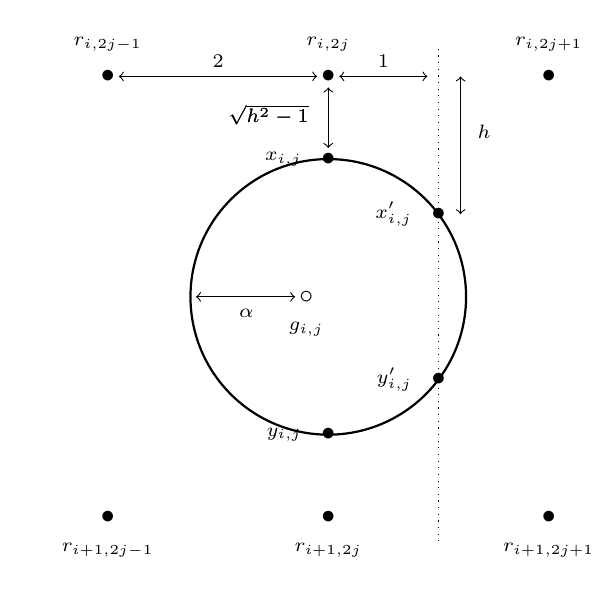
\begin{tikzpicture}[scale=7]

	
	\node[label=90:\scriptsize $r_{i,2j-1}$] at (0.1,0) {$\bullet$};
	\node[label=90:\scriptsize $r_{i,2j}$] at (0.5,0) {$\bullet$};
	\node[label=90:\scriptsize $r_{i,2j+1}$] at (0.9,0) {$\bullet$};
	
	\node[label=180:\scriptsize $\sqrt{h^2-1}$] at (0.5,-0.07) {};
	\node[label=180:\scriptsize $x_{i,j}$] at (0.5,-0.15) {$\bullet$};
	
	
	\node[label=180:\scriptsize $h$] at (0.83,-0.1) {};
	\node[label=180:\scriptsize $x_{i,j}'$] at (0.7,-0.25) {$\bullet$};
	
	\node[label=270:\scriptsize $g_{i,j}$] at (0.46,-0.4) {$\circ$};
	
	
	\node[label=180:\scriptsize $y_{i,j}$] at (0.5,-0.65) {$\bullet$};
	\node[label=180:\scriptsize $y_{i,j}'$] at (0.7,-0.55) {$\bullet$};
	
	
	\node[label=270:\scriptsize $r_{i+1,2j-1}$] at (0.1,-0.8) {$\bullet$};
	\node[label=270:\scriptsize $r_{i+1,2j}$] at (0.5,-0.8) {$\bullet$};
	\node[label=270:\scriptsize $r_{i+1,2j+1}$] at (0.9,-0.8) {$\bullet$};
	
	
	\node[label=180:\scriptsize $\sqrt{h^2-1}$] at (0.5,-0.07) {};
	
	
	\node[label=180:\scriptsize $\alpha$] at (0.4,-0.43) {};
	\node[label=90:\scriptsize $1$] at (0.6,-0.02) {};
	\node[label=90:\scriptsize $2$] at (0.3,-0.02) {};
	
	
	\draw[<->] (0.5,-0.13) -- (0.5,-0.02);
	\draw[<->] (0.26,-0.4) -- (0.44,-0.4);
	\draw[dotted,-] (0.7, 0.05) -- (0.7, -0.85);
	\draw[<->] (0.74, 0.0) -- (0.74, -0.25);
	\draw[<->] (0.68, 0.0) -- (0.52, 0.0);
	\draw[<->] (0.12, 0.0) -- (0.48, 0.0);
	\draw[black, thick] (0.5,-0.4) circle (0.25);
\end{tikzpicture}


\ifdefined\ACCOMPLETE
\else
\end{document}
\fi

    \caption{The locations of $x_{i,j}$, $x_{i,j}'$, $y_{i,j}$ and $y_{i,j}'$ in the set $Z_i$. Note that the point $g_{i,j}$ is not vertically aligned with $x_{i, j}$ or $r_{i, 2j}$. This figure is adapted from \cite{vattani2009hardness}.}
    \label{fig:ZFig}
  \end{minipage}
\end{figure}

\subsection{Reduction design}
Given an instance of X3C, that is the elements $U = \{1, \ldots, 3m\}$ and the collection $\mc S$, we construct a set of points $X$ in the Euclidean plane which we want to cluster. Particularly, $X$ consists of a set of points $H_{l,m}$ in a grid-like manner, and the sets $Z_i$ corresponding to $S_i$. In other words, $X = H_{l,m} \cup (\cup_{i=1}^{l-1} Z_i)$. 

The set $H_{l,m}$ is as described in Fig. \ref{fig:lowerBoundComponent}. The row $R_i$ is composed of $6m + 3$ points $\{s_i, r_{i, 1}, \ldots, r_{i, 6m+1}, f_i\}$. Row $G_i$ is composed of $3m$ points $\{g_{i,1}, \ldots, g_{i, 3m}\}$. The distances between the points are also shown in Fig. \ref{fig:lowerBoundComponent}. Also, all these points have weight $w$, simply meaning that each point is actually a set of $w$ points on the same location.

Each set $Z_i$ is constructed based on $S_i$. In particular, $Z_i = \cup_{j\in [3m]} B_{i,j}$, where $B_{i,j}$ is a subset of $\{x_{i,j},x_{i,j}',y_{i,j},y_{i,j}'\}$ and is constructed as follows: $x_{i,j} \in B_{i,j}$ iff $j \not\in S_i$, and $x_{i,j}' \in B_{i,j}$ iff $j \in S_i$. Similarly,  $y_{i,j} \in B_{i,j}$ iff $j \not\in S_{i+1}$, and $y_{i,j}' \in B_{i,j}$ iff $j \in S_{i+1}$. Furthermore, $x_{i, j}, x_{i,j}^\prime, y_{i,j}$ and $y_{i, j}^\prime$ are specific locations as depicted in Fig. \ref{fig:ZFig}. In other words, exactly one of the locations $x_{i,j}$ and $x_{i,j}^\prime$, and one of $y_{i,j}$ and $y_{i,j}^\prime$ will be occupied. We set the following parameters. 
\vspace{-0.1in}
\begin{align*}
&h = \sqrt{5}, d = \sqrt{6}, \epsilon = \frac{1}{w^2}, \lambda = \frac{2}{\sqrt{3}}h, k = (l-1)3m + l(3m+2)\\
& L_1 = (6m+3)wl, L_2 = 3m(l-1)w, L = L_1 + L_2 - m\alpha, \alpha = \frac{d}{w}-\frac{1}{2w^3}
\end{align*}


\begin{lemma}
\label{lemma:kmeansEquivalenceX3C}
The set $X = H_{l,n} \cup Z$ has a $k$-clustering of cost less or equal to $L$ if and only if there is an exact cover for the X3C instance.
\end{lemma}

\begin{lemma}
\label{lemma:gammaLower}
Any $k$-clustering of $X = H_{l,n} \cup Z$ with cost $\le L$ has the $\gamma$-margin property where $\gamma = \sqrt{3.4}$. Furthermore, $k = \Theta(n^{\epsilon})$.
\end{lemma}

The proofs are provided in Appendix \ref{appendix:lowerBoundProof}. Lemmas \ref{lemma:kmeansEquivalenceX3C} and \ref{lemma:gammaLower} together show that $X$ has a $k$-clustering of cost $\le L$ satisfying the $\gamma$-margin property (for $\gamma = \sqrt{3.4}$) if and only if there is an exact cover by $3$-sets for the X3C instance. This completes the proof of our main result (Thm. \ref{thm:gammaLower}). 

\section{Conclusions and Future Directions}
In this work we introduced a framework for semi-supervised clustering with same-cluster queries. Those queries can be viewed as a natural way for a clustering mechanism to gain domain knowledge, without which clustering is an under-defined task. The focus of our analysis was the computational and query complexity of %clustering in this  Then query complexity and computational complexity of 
such problems, when the input data set satisfies a clusterability condition -- the $\gamma$-margin property.

Our main result shows that access to a limited number of such query answers (logarithmic in the size of the data set and quadratic in the number of clusters) allows efficient successful clustering under conditions (margin parameter between 1 and $\sqrt{3.4} \approx 1.84$) that render the problem NP-hard without the help of such a query mechanism.  
 
With practical applications of clustering in mind, a natural extension of our model is to allow the oracle (i.e., the domain expert) to refrain from answering a certain fraction of the queries, or to make a certain number of errors in its answers. It would be interesting to analyze how the performance guarantees of query-based algorithms behave as a function of such abstentions and error rates. 

\ifdefined\COMPLETE
\else
\end{document}
\fi

\begin{subappendices}
\def\COMPLETE{}
\section{Relationships Between Query Models}
\label{appendix:diffQueryModels}

\begin{proposition}
Any clustering algorithm that uses only $q$ same-cluster queries can be adjusted to use $2q$ cluster-assignment queries (and no same-cluster queries) with the same order of time complexity.
\end{proposition}
\begin{proof}
We can replace each same-cluster query with two cluster-assignment queries as in $Q(x_1,x_2)={\mathbbm{1}}\{Q(x_1)=Q(x_2))\}$.
\end{proof}

\begin{proposition}
Any algorithm that uses only $q$ cluster-assignment queries can be adjusted to use $kq$ same-cluster queries (and no cluster-assignment queries) with at most a factor $k$ increase in computational complexity, where $k$ is the number of clusters.
\end{proposition}
\begin{proof}
If the clustering algorithm has access to an instance from each of $k$ clusters (say $x_i\in X_i$), then it can simply simulate the cluster-assignment query by making $k$ same-cluster queries ($Q(x) = \argmax_{i}\mathbbm{1}\{Q(x, x_i)\}$). Otherwise, assume that at the time of querying $Q(x)$ it has only instances from $k^\prime<k$ clusters. In this case, the algorithm can do the same with the $k^\prime$ instances and if it does not find the cluster, assign $x$ to a new cluster index. This will work, because in the clustering task the output of the algorithm is a partition of the elements, and therefore the indices of the clusters do not matter.
\end{proof}


%-----------------------------------------------------------
%-----------------------------------------------------------
%-----------------------------------------------------------


\section{Comparison of $\gamma$-Margin and $\alpha$-Center Proximity}
\label{appendix:gammaMrginVsAlphaCenter}

In this paper, we introduced the notion of $\gamma$-margin niceness property. We further showed upper and lower bounds on the computational complexity of clustering under this assumption. It is therefore important to compare this notion with other previously-studied clusterability notions.

%, and provided upper (with query) and lower bounds on $\gamma$, when the metric space $M$ is Euclidean and the centers are allowed to be points in the metric space. 

An important notion of niceness of data for clustering is $\alpha$-center proximity property.

\begin{definition}[$\alpha$-center proximity \cite{awasthi2012center}]
\label{defn:alphacp}
Let $(\mc X, d)$ be a clustering instance in some metric space $M$, and let $k$ be the number of clusters. We say that a center-based clustering $\mc C = \{C_1, \ldots, C_k\}$ induced by centers $c_1, \ldots, c_k \in M$ satisfies the $\alpha$-center proximity property (with respect to  $\mc X$ and $k$) if the following holds 
$$\forall x \in C_i, i\neq j, \alpha d(x, c_i) < d(x, c_j)$$
\end{definition}


 This property has been considered in the past in various studies \cite{balcan2012clustering,awasthi2012center}. In this appendix we will show some connections between $\gamma$-margin and $\alpha$-center proximity properties.
 
 
  It is important to note that throughout this paper we considered clustering in Euclidean spaces. Furthermore, the centers were not restricted to be selected from the data points. 
  However, this is not necessarily the case in other studies.





\begin{table}[]
\centering
\caption{Known results for $\alpha$-center proximity}
\label{table:alphacp}
\begin{tabular}{lll}
\cline{2-3}
\multicolumn{1}{l|}{} & \multicolumn{1}{l|}{Euclidean} & \multicolumn{1}{l|}{General Metric} \\ \hline
\multicolumn{1}{|l|}{\begin{tabular}[c]{@{}l@{}}Centers \\ from data\end{tabular}} & \multicolumn{1}{l|}{\begin{tabular}[c]{@{}l@{}}Upper bound : $\sqrt{2}+1$  \cite{balcan2012clustering}\\ Lower bound : ?\end{tabular}} & \multicolumn{1}{l|}{\begin{tabular}[c]{@{}l@{}}Upper bound : $\sqrt{2}+1$  \cite{balcan2012clustering}\\ Lower bound : 2 \cite{ben2014data}\end{tabular}} \\ \hline
\multicolumn{1}{|l|}{\begin{tabular}[c]{@{}l@{}}Unrestricted \\ Centers \end{tabular}} & \multicolumn{1}{l|}{\begin{tabular}[c]{@{}l@{}}Upper bound : $2+\sqrt{3}$ \cite{awasthi2012center}\\ Lower bound : ?\end{tabular}} & \multicolumn{1}{l|}{\begin{tabular}[c]{@{}l@{}}Upper bound : $2+\sqrt{3}$ \cite{awasthi2012center}\\ Lower bound : 3 \cite{awasthi2012center}\end{tabular}} \\ \hline
 &  & 
\label{table:alphacenter}
\end{tabular}
\end{table}

An overview of the known results under $\alpha$-center proximity is provided in Table \ref{table:alphacenter}. The results are provided for the case that the centers are restricted to be selected from the training set, and also the unrestricted case (where the centers can be arbitrary points from the metric space). Note that any upper bound that works for general metric spaces also works for the Euclidean space. 

We will show that using the same techniques one can prove upper and lower bounds for $\gamma$-margin property. It is important to note that for $\gamma$-margin property, in some cases the upper and lower bounds match. Hence, there is no hope to further improve those bounds unless P=NP. A summary of our results is provided in \ref{table:gammamargin}.  

\begin{table}[]
\centering
\caption{Results for $\gamma$-margin}
\label{table:gammamargin}
\begin{tabular}{lll}
\cline{2-3}
\multicolumn{1}{l|}{}                                                                     & \multicolumn{1}{l|}{Euclidean} & \multicolumn{1}{l|}{General Metric}                                                                         \\ \hline
\multicolumn{1}{|l|}{\begin{tabular}[c]{@{}l@{}}Centers \\ from data\end{tabular}}        & \multicolumn{1}{l|}{\begin{tabular}[c]{@{}l@{}}Upper bound : 2 (Thm. \ref{thm:upperCenterData})\\ Lower bound : ? \end{tabular}}    &       \multicolumn{1}{l|}{\begin{tabular}[c]{@{}l@{}}Upper bound : 2 (Thm. \ref{thm:upperCenterData})\\ Lower bound : 2 (Thm. \ref{thm:lowerCenterData})\end{tabular}}           \\ \hline
\multicolumn{1}{|l|}{\begin{tabular}[c]{@{}l@{}}Unrestricted \\Centers \end{tabular}} & \multicolumn{1}{l|}{\begin{tabular}[c]{@{}l@{}}Upper bound : 3 (Thm. \ref{thm:upperCenterMetric})\\ Lower bound : 1.84 (Thm. \ref{thm:gammaLower})\\ \end{tabular}}         & \multicolumn{1}{l|}{\begin{tabular}[c]{@{}l@{}}Upper bound : 3 (Thm. \ref{thm:upperCenterMetric})\\ Lower bound : 3 (Thm. \ref{thm:lowerCenterMetric})\end{tabular}} \\ \hline
                                                                                          &                       &    
\label{table:gammamargin}                                                                                                                                                                                                 
\end{tabular}
\end{table}

\subsection{Centers from data}
\begin{theorem}
\label{thm:upperCenterData}
Let $(X , d)$ be a clustering instance and $\gamma \ge 2$. Then, Algorithm 1 in \cite{balcan2012clustering} outputs a tree $\mc T$ with the following property: 


Any $k$-clustering $\mc C^* = \{C_1^*, \ldots, C_k^* \}$ which satisfies the $\gamma$-margin property and its cluster centers $\mu_1, \ldots, \mu_k$ are in $X$, is a pruning of the tree $T$. In other words, for every $1 \le i \le k$, there exists a node $N_i$ in the tree $T$ such that $C_i^* = N_i$.
\end{theorem}

\begin{proof}
Let $p, p' \in C_i^*$ and $q \in C_j^*$. \cite{balcan2012clustering} prove the correctness of their algorithm for $\alpha > \sqrt{2} + 1$. Their proof relies only on the following three properties which are implied when $\alpha > \sqrt{2} + 1$. We will show that these properties are implied by $\gamma > 2$ instances as well.
\begin{itemize}[nolistsep,noitemsep]
\item $d(p, \mu_i) < d(p, q)$\\
$\gamma d(p, \mu_i) < d(q, \mu_i) < d(p, q) + d(p, \mu_i) \implies d(p, \mu_i) < \frac{1}{\gamma-1}d(p, q)$.
\item $d(p, \mu_i) < d(q, \mu_i)$\\
This is trivially true since $\gamma > 2$.
\item $d(p, \mu_i) < d(p', q)$\\
Let $r = \max_{x \in C_i^*} d(x, \mu_i)$. Observe that $d(p, \mu_i) < r$. Also, $d(p', q)> d(q, \mu_i)-d(p', \mu_i) > \gamma r - r = (\gamma -1)r$.
\end{itemize}
\end{proof}

\begin{theorem}
\label{thm:lowerCenterData}
Let $(\mc X, d)$ be a clustering instance and $k$ be the number of clusters. For $\gamma < 2$, finding a $k$-clustering of $X$ which satisfies the $\gamma$-margin property and where the corresponding centers $\mu_1, \ldots, \mu_k$ belong to $\mc X$ is NP-Hard.
\end{theorem}
\begin{proof}
For $\alpha < 2$, \cite{ben2014data} proved that in general metric spaces, finding a clustering which satisfies the $\alpha$-center proximity and where the centers $\mu_1, \ldots, \mu_k \in \mc X$ is NP-Hard. Note that the reduced instance in their proof, also satisfies $\gamma$-margin for $\gamma < 2$. 
\end{proof}

\subsection{Centers from metric space}
\begin{theorem}
\label{thm:upperCenterMetric}
Let $(X , d)$ be a clustering instance and $\gamma \ge 3$. Then, the standard single-linkage algorithm outputs a tree $\mc T$ with the following property:


Any $k$-clustering $\mc C^* = \{C_1^*, \ldots, C_k^* \}$ which satisfies the $\gamma$-margin property is a pruning of $T$. In other words, for every $1 \le i \le k$, there exists a node $N_i$ in the tree $T$ such that $C_i^* = N_i$. 
\end{theorem}

\begin{proof}
\cite{balcan2008discriminative} showed that if a clustering $C^*$ has the strong stability property, then single-linkage outputs a tree with the required property. It is simple to see that if $\gamma > 3$ then instances have strong-stability and the claim follows.  
\end{proof}


\begin{theorem}
\label{thm:lowerCenterMetric}
Let $(\mc X, d)$ be a clustering instance and $\gamma < 3$. Then, finding a $k$-clustering of $X$ which satisfies the $\gamma$-margin is NP-Hard.
\end{theorem}
\begin{proof}
\cite{awasthi2012center} proved the above claim but for $\alpha < 3$ instances. Note however that the construction in their proof satisfies $\gamma$-margin for $\gamma < 3$. 
\end{proof}



%-----------------------------------------------------------
%-----------------------------------------------------------
%-----------------------------------------------------------

\section{Proofs of Lemmas \ref{lemma:kmeansEquivalenceX3C} and \ref{lemma:gammaLower}}
\label{appendix:lowerBoundProof}

In Section \ref{section:lowerBounds} we proved Theorem \ref{thm:gammaLower} based on two technical results (i.e., lemma \ref{lemma:kmeansEquivalenceX3C} and \ref{lemma:gammaLower}). In this appendix we provide the proofs for these lemmas. In order to start, we first need to establish some properties about the Euclidean embedding of $X$ proposed in Section \ref{section:lowerBounds}.

%$$L_1 = (6m+3)w, L_2 = 6m(l-1), L=L_1 + L_2, \alpha = \frac{d}{w}-\frac{1}{2w^3}$$

\begin{definition}[$A$- and $B$-Clustering of $R_i$]
\label{defn:abclusteringVattani}

An $A$-Clustering of row $R_i$ is a clustering in the form of $\{\{s_i\}, \{r_{i,1}, r_{i,2}\}, \{r_{i,3}, r_{i,4}\}, \ldots,$ $ \{r_{i,6m-1}, r_{i,6m}\},\{r_{i, 6m+1}, f_i\}\}$. A $B$-Clustering of row $R_i$ is a clustering in the form of $\{\{s_i, r_{i, 1}\}, \{r_{i,2}, r_{i,3}\}, \{r_{i,4}, r_{i,5}\}, \ldots,$ $ \{r_{i,6m}, r_{i,6m+1}\},\{f_i\}\}$. 
\end{definition}

\begin{definition}[Good point for a cluster]
\label{defn:goodPointVattani}
A cluster $C$ is good for a point $z \not\in C$ if adding $z$ to $C$ increases cost by exactly $\frac{2w}{3}h^2$ 
\end{definition}

Given the above definition, the following simple observations can be made. 
\begin{itemize}[nolistsep,noitemsep]
\item The clusters $\{r_{i,2j-1}, r_{i, 2j}\}$, $\{r_{i,2j}, r_{i, 2j+1}\}$ and $\{g_{i,j}\}$ are good for $x_{i,j}$ and $y_{i-1,j}$.
\item The clusters $\{r_{i,2j}, r_{i, 2j+1}\}$ and $\{g_{i,j}\}$ are good for $x_{i,j}'$ and $y_{i-1,j}'$.
\end{itemize}

\begin{definition}[Nice Clustering]
\label{defn:niceClustering}
A $k$-clusteirng is nice if every $g_{i,j}$ is a singleton cluster, each $R_i$ is grouped in the form of either an $A$-clustering or a $B$-clustering, and each point in $Z_i$ is added to a cluster which is good for it.
\end{definition}

It is straightforward to see that a row grouped in a $A$-clustering costs $(6m+3)w-\alpha$ while a row in $B$-clustering costs $(6m+3)w$. Hence, a nice clustering of $H_{l,m} \cup Z$ costs at most $L_1 + L_2$. More specifically, if $t$ rows are group in a $A$-clustering, the nice-clustering costs $L_1+L_2-t\alpha$. Also, observe that any nice clustering of $X$ has only the following four different types of clusters. \begin{enumerate}[label=(\arabic*),nolistsep,leftmargin=*]
\item Type E - $\{r_{i,2j-1}, r_{i,2j+1}\}$ \\
The cost of this cluster is $2w$ and the contribution of each location to the cost (i.e., $\frac{cost}{\#locations}$) is $ \frac{2w}{2} = w$.
\item Type F - $\{r_{i,2j-1}, r_{i, 2j}, x_{i, j}\}$ or $\{r_{i,2j-1}, r_{i, 2j}, y_{i-1, j}\}$ or $\{r_{i,2j}, r_{i, 2j+1}, x_{i, j}'\}$ or $\{r_{i,2j}, r_{i, 2j+1}, y_{i-1, j}'\}$\\
The cost of any cluster of this type is $2w(1+\frac{h^2}{3})$ and the contribution of each location to the cost is at most $\frac{2w}{9}(h^2+3)$. This is equal to $\frac{16}{9}w$ because we had set $h = \sqrt 5$.
\item Type I - $\{g_{i, j}, x_{i,j}\}$ or $\{g_{i, j}, x_{i,j}'\}$  or $\{g_{i, j}, y_{i,j}\}$  or $\{g_{i, j}, y_{i,j}'\}$\\
The cost of any cluster of this type is $\frac{2}{3}wh^2$ and the contribution to the cost of each location is $\frac{w}{3}h^2$. For our choice of $h$, the contribution is $\frac{5}{3}w$.
\item Type J - $\{s_i, r_{i,1}\}$ or $\{r_{i,6m+1}, f_i\}$\\
The cost of this cluster is $3w$ (or $3w-\alpha$) and the contribution of each location to the cost is at most $1.5w$. 
\end{enumerate}
Hence, observe that in a nice-clustering, any location contributes at most $\le \frac{16}{9}w$ to the total clustering cost. This observation will be useful in the proof of the lemma below.

\begin{lemma}
\label{lemma:costNonNice}
For large enough $w = poly(l, m)$, any non-nice clustering of $X = H_{l, m} \cup Z$ costs at least $L + \frac{w}{3}$.
\end{lemma}

\begin{proof}
We will show that any non-nice clustering $C$ of $X$ costs at least $\frac{w}{3}$ more than any nice clustering. This will prove our result. The following cases are possible.

\begin{itemize}[nolistsep,leftmargin=*]
\item $C$ contains a cluster $C_i$ of cardinality $t > 6$ (i.e., contains $t$ weighted points)\\
Observe that any $x \in C_i$ has at least $t-5$ locations at a distance greater than 4 to it, and $4$ locations at a distance at least $2$ to it. Hence, the cost of $C_i$ is at least $\frac{w}{2t}(4^2(t-5)+2^24)t = 8w(t-4)$. $C_i$ allows us to use at most $t-2$ singletons. This is because a nice clustering of these $t+(t-2)$ points uses at most $t-1$ clusters and the clustering $C$ uses  $1 + (t-2)$ clusters for these points. The cost of the nice cluster on these points is $\le \frac{16w}{9}2(t-1)$. While the non-nice clustering costs at least $8w(t-4)$. For $t \ge 6.4 \implies 8(t-4) > \frac{32}{9}(t-1)$ and the claim follows. Note that in this case the difference in cost is at least $\frac{8w}{3}$. 

\item Contains a cluster of cardinality $t = 6$\\
Simple arguments show that amongst all clusters of cardinality $6$, the following has the minimum cost. $C_i = \{r_{i, 2j-1}, r_{i, 2j}, x_{i,j}, y_{i-1, j}, r_{i, 2j+1}, r_{2j+2}\}$. The cost of this cluster is $\frac{176w}{6}$. Arguing as before, this allows us to use $4$ singletons. Hence, a nice cluster on these $10$ points costs at most $\frac{160w}{9}$. The difference of cost is at least $34w$.  

\item Contains a cluster of cardinality $t = 5$\\
Simple arguments show that amongst all clusters of cardinality $5$, the following has the minimum cost. $C_i = \{r_{i, 2j-1}, r_{i, 2j}, x_{i,j}, y_{i-1, j}, r_{i, 2j+1}\}$. The cost of this cluster is $16w$. Arguing as before, this allows us to use $3$ singletons. Hence, a nice cluster on these $8$ points costs at most $16w\frac{8}{9}$. The difference of cost is at least $\frac{16w}{9}$.  

\item Contains a cluster of cardinality $t = 4$\\
It is easy to see that amongst all clusters of cardinality $4$, the following has the minimum cost. $C_i = \{r_{i, 2j-1}, r_{i, 2j}, x_{i,j}, r_{i, 2j+1}\}$. The cost of this cluster is $11w$. Arguing as before, this allows us to use $2$ singletons. Hence, a nice cluster on these $6$ points costs at most $\frac{32w}{3}$. The difference of cost is at least $\frac{w}{3}$.

\item All the clusters have cardinality $\le 3$ \\
Observe that amongst all non-nice clusters of cardinality $3$, the following has the minimum cost. $C_i = \{r_{i, 2j-1}, r_{i, 2j}, r_{i, 2j+1}\}$. The cost of this cluster is $8w$. Arguing as before, this allows us to use at most $1$ more singleton. Hence, a nice cluster on these $4$ points costs at most $\frac{64w}{9}$. The difference of cost is at least $\frac{8w}{9}$.

It is also simple to see that any non-nice clustering of size $2$ causes an increase in cost of at least $w$.

\end{itemize}
\end{proof}

%\begin{lemma}
%\label{lemma:kmeansEquivalenceX3C}
%The set $X = H_{l,n} \cup Z$ has a $k$-clustering %of cost less or equal to $L$ if and only if there %is an exact cover for the X3C instance.
%\end{lemma}
\begin{proof}[Proof of lemma \ref{lemma:kmeansEquivalenceX3C}]
The proof is identical to the proof of Lemma 11 in \cite{vattani2009hardness}. Note that the parameters that we use are different with those utilized by \cite{vattani2009hardness}; however, this is not an issue, because we can invoke our lemma \ref{lemma:costNonNice} instead of the analogous result in Vattani (i.e., lemma 10 in Vattani's paper). The sketch of the proof is that based on lemma \ref{lemma:costNonNice}, only nice clusterings of $X$ cost $\le L$. On the other hand, a nice clustering corresponds to an exact 3-set cover. Therefore, if there exists a clustering of $X$ of cost $\le L$, then there is an exact 3-set cover. The other way is simpler to proof; assume that there exists an exact 3-set cover. Then, the corresponding construction of $X$ makes sure that it will be clustered \emph{nicely}, and therefore will cost $\le L$.  



 %argue why the only nice clusterings of $X$ cost $\le L$. We use Lemma \ref{lemma:costNonNice} to argue the same. Note that since the parameters are much different that those considered in Vattani's original construction, we need to argue much more carefully to prove Lemma \ref{lemma:costNonNice}. 
\end{proof}

%\begin{lemma}
%\label{lemma:gammaLower}
%Any clustering of $X = H_{l,n} \cup Z$ which has %cost$\le L$ has the $\gamma$-margin property where %$\gamma = \sqrt{\frac{17}{5}} \approx 1.84$.
%\end{lemma}
\begin{proof}[Proof of lemma \ref{lemma:gammaLower}]
As argued before, any nice clustering has four different types of clusters. We will calculate the minimum ratio $a_i = \frac{d(y, \mu)}{d(x, \mu)}$ for each of these clusters $C_i$ (where $x \in C_i$, $y \not\in C_i$ and $\mu$ is mean of all the points in $C_i$.) Then, the minimum $a_i$ will give the desired $\gamma$. 
\begin{enumerate}[label=(\arabic*),nolistsep,leftmargin=*]
\item For Type E clusters $a_i = h/1 = \sqrt{5}$. 
\item For Type F clusters. $a_i = \frac{\frac{\sqrt{4+16(h^2-1)}}{3}}{2h/3} = \sqrt{\frac{17}{5}} \approx 1.84$. 
\item For Type I clusters, standard calculation show that $a_i > 2$.
\item For Type J clusters $a_i = \frac{2+\frac{\sqrt{6}}{2}}{\frac{\sqrt{6}}{2}} > 2$.
\end{enumerate}

\noindent Furthurmore, $|\mc X| = (12lm + 3l -6m)w$ and $k = 6lm + 2l - 3m$. Hence for $w = $poly$(l, m)$ our hardness result holds for $k = |\mc X|^{\epsilon}$ for any $0 < \epsilon < 1$.
\end{proof}
\noindent Lemmas \ref{lemma:kmeansEquivalenceX3C} and \ref{lemma:gammaLower} complete the proof of the main result (Thm. \ref{thm:gammaLower}). 

\end{subappendices}

\chapter{Semi-supervised clustering for deduplication}
\label{chapter:deduplication}
\ifdefined\COMPLETE
\else
\documentclass[12pt]{article}

\usepackage{amsmath,amsthm,mathtools}
\usepackage{graphicx}
\usepackage{algorithm2e}
\usepackage{thm-restate}

\usepackage{tikz}
\usetikzlibrary{shapes, calc, arrows, through, intersections, decorations.pathreplacing, patterns}

\newtheorem{theorem}{Theorem}
\newtheorem{definition}[theorem]{Definition}
\newtheorem{thrm}[theorem]{Theorem}
\newtheorem{lem}[theorem]{Lemma}
\newtheorem{corollary}[theorem]{Corollary}

\newcommand{\mb}{\mathbf}
\newcommand{\mc}{\mathcal}
\newcommand\numberthis{\addtocounter{equation}{1}\tag{\theequation}}
\let\oldnl\nl
\newcommand{\nonl}{\renewcommand{\nl}{\let\nl\oldnl}}

\DeclareMathOperator*{\argmin}{arg\,min}
\DeclareMathOperator*{\vcdim}{VC-Dim}

\begin{document}
\fi

\section{Introduction}
Record de-duplication is a central task in data cleaning in large data bases. Common practical examples include the detection of records referring to the same patient in large health data bases (different records might have been generated for same patient in different clinics or even in the same clinic at different times), detecting same person records in census data, detecting customer records, duplicate records of papers in Google Scholar and so on and so forth \cite{elmagarmid2007duplicate}, \cite{chu2016distributed}, \cite{ilyas2015trends}.

Since the same-entity relation is reflexive symmetric and transitive, the sets of duplicate records can be viewed as clusters. Consequently, the record de-duplication task can be viewed as a clustering task. Such a clustering task has several characteristics that make it hard to address with common clustering tools; The number of ground truth clusters is unknown to the algorithm. Furthermore, one cannot a priory bias the algorithm towards a larger or a smaller number of clusters (unlike, say, facility location tasks in which it makes sense to trade off cluster cohesiveness with the number of clusters). This implies that attempts to use standard classification prediction learning tools to predict which pairs or records should be labelled `same-cluster' and which should be `different clusters' (D) are bound to fail - uniformly drawn samples of pairs are likely to be all labeled D and the resulting constant "all D" classifier will have negligible $0-1$ error over the set of pairs. On top of that all, there is no a priori geometry to the clusters structure, one cannot justify common simplifying assumptions like some stability of the clustering, some convexity of the larger-than-two sized clusters  or significant between-clusters margins.

The framework of correlation clustering extends naturally to the data de-duplication problem. Given a complete graph $G$ vertices where each edge is labelled as a $1$ or a $0$, the goal is to cluster the vertices of the graph so as to correlate “as much as possible” to the edges of the graph. That is find a clustering so as to minimize the number of $0$ edges within a cluster plus the number of $1$ edges across different clusters (or correlation loss). An edge label $0$ indicates that the two records have been deemed to be different while $1$ indicates that the records are similar. However, finding the clustering with minimum correlation loss is known to be NP-Hard \cite{bansal2004correlation}. 

One characteristic of record de-duplication which makes it different from other clustering tasks is the applicability of `human supervision'. For example, given two records from a medical database or two papers from DBLP or two citizens from a census data, it is fairly easy for a human to identify whether these records refer to the same physical entity. The framework of correlation clustering does not take this into account. Most prevalent approaches for data de-duplication are based on designing a similarity measure (or distance) over the records, such that records that are highly similar according to that measure are likely to be duplicate and records that measure as significantly dissimilar are likely to represent different entities. In other words, the edge labels are `close to' the underlying ground truth clustering. This is another aspect of data de-duplication which the current correlation clustering framework does not take into account. 
  
In this paper we offer a formal modelling of such record de-duplication tasks. Our framework is the same as correlation clustering but with the added \textit{promise} that the input graph edges $E$ is `close to' the optimal correlation clustering of the given dataset. We analyse the computational complexity of this problem and show that even under strong promise, correlation clustering is NP-Hard. Moreover, the problem remains NP-Hard even when we are allowed to make queries to a human expert (or an \textit{oracle}) as long as the number of queries is not too large (less than the number of points in the dataset). 

Given these negative results, we propose a \textit{restricted} variant of correlation clustering. Here, instead of finding the best clustering from the class of all possible clusterings, the learning algorithm has to choose the best clustering from a given class $\mc F$ of clusterings. We offer an algorithmic approach (which uses the help of an oracle) with success guarantees for the restricted version. The `success guarantee' depends on the complexity of the class $\mc F$ (measured by $\vcdim(\mc F)$) as well as the `closeness' of the metric $d$ to the target clustering.  

\subsection{Related Work}
The most relevant work is the framework of correlation clustering developed by \cite{bansal2004correlation} that we discussed in the previous section. Other variations of correlation clustering have been considered. For example \cite{demaine2006correlation}, consider a problem where the edges can be labelled by a real number instead of just $0$ or $1$. Edges with large positive weights encourage those vertices to be in the same cluster while edges with large negative weights encourage those points to be in different clusters. They showed that the problem is NP-Hard and gave a $O(\log n)$ approximation to the weighted correlation clustering problem. \cite{charikar2005clustering} made several contributions to the correlation clustering problem. For the problem of minimizing the correlation clustering loss (for unweighted complete graphs), they gave an algorithm with factor $4$ approximation. They also proved that the minimization problem is APX-Hard. 

More recently, \cite{ailon2018approximate} considered the problem of correlation clustering in the presence of an oracle. If the number of clusters $k$ is known, they proposed an algorithm which makes $O(k^{14} \log n)$ queries to the oracle and finds a $(1+\epsilon)$-approximation to the correlation clustering problem. They showed that the problem is NP-Hard to approximate with $o\big(\frac{k}{poly \log k}\big)$ queries to an oracle. In this work, we obtain similar results for the {promise correlation clustering} problem.

Supervision in clustering has been addressed before. For example, \cite{kulis2009semi,basu2004probabilistic,basu2002semi} considered {\em link/don't-link} constraints. This is a form of non-interactive clustering where the algorithm gets as input a list of pairs which should be in the same cluster and a list pairs which should be in different clusters. \cite{balcan2008clustering} developed a framework of interactive clustering where the supervision is provided in the form of {\em split/merge} queries. The algorithm gives the current clustering to the oracle. The oracle responds by telling the which clusters to merge and which clusters to split. 

In this work, we use the framework of same-cluster queries developed by \cite{ashtiani2016clustering}. At any given instant, the clustering algorithm asks the same-cluster oracle about two points in the dataset. The oracle replies by answering either `yes' or `no' depending upon whether the two points lie in the same or different clusters. 

On de-duplication side, most prevalent are approaches that are based on designing a similarity measure (or distance) over the records, such that records that are highly similar according to that measure are likely to be duplicates and records that measure as significantly dissimilar are likely to represent different entities. For example, to handle duplicate records created due typographical mistakes, many character-based similarity metrics have been considered. Examples of such metrics include the edit or levenshtein distance \cite{levenshtein1966binary}, smith-waterman distance \cite{waterman1981identification} and jaro distance metric \cite{jaro1980unimatch}. Token-based similarity metrics try to handle rearrangement of words, for example \cite{monge1996field} and \cite{cohen1998integration}. Other techniques include phonetic-based metrics and numerical metrics (to handle numeric data). A nice overview of these methods can be found in \cite{elmagarmid2007duplicate}. 
   
While the above approaches relied on designing a good similarity metric, some works try to `learn' the distance function from a labelled training dataset of pairs of records. Examples of such works include \cite{cochinwala2001efficient} and \cite{bilenko2003adaptive}. Clustering for de-duplication has been mostly addressed in application oriented works. \cite{hernandez1995merge} assumes that the duplicate records are transitive. The clustering problem now reduces to finding the connected components in a graph. 

\subsection{Outline}
Section \ref{section:problemFormulation} introduces the relevant notation and definitions. In Section \ref{section:PCC}, we introduce our framework of Promise Correlation Clustering. In Section \ref{section:PCCNPHard}, we prove that PCC is NP-Hard. In Section \ref{section:PCCNPHardOracle} we prove that PCC is NP-Hard even under the presence of an oracle. In Section \ref{section:RCC}, we introduce our framework of Restricted Correlation Clustering (RCC). In Sections \ref{section:samplingNegative} and \ref{section:samplingPositive} we describe procedures for sampling different-cluster (negative) and same-cluster (positive) pairs. In Section \ref{section:sampleAndQueryComplexity}, we describe our semi-supervised algorithm for solving the RCC problem. We prove an upper bound on the number of labelled samples required to guarantee the success of our algorithm. We also upper bound the number of queries made to the same-cluster oracle. Section \ref{section:conclusion} concludes our work. All the missing proofs can be found in the supplementary section. 

\section{Preliminaries}
\label{section:problemFormulation}
Given a finite domain $X$. A clustering $C$ of the set $X$ is a partition of the set $X$ into $k$ disjoint subsets, that is, $C = \{C_1, \ldots, C_k\}$. Denote by $m(C) = \max C_i$. Define $X^{[2]} = \{(x, y) : x \neq y\}$. In this paper, we view a clustering as a binary-valued function over the pairs of instances. That is, $C: X^{[2]} \rightarrow \{0, 1\}$ and $C(x, y) = 1$ if and only if $x, y$ are in the same $C$ cluster. 

Given $G = (X, E)$, define $d_E(x, y) = 0$ if there exists an edge between $x, y$ and $d_E(x, y) = 1$ otherwise. 

\begin{definition}[Correlation clustering for deduplication]\cite{bansal2004correlation}
Given $G = (X, E)$, find a clustering $C$ which minimizes 
\begin{align*}
  &L_{d_E}(C) = NL_{d_E}(C) + PL_{d_E}(C), \text{ where}\\
  &NL_{d_E}(C) = |\{(x, y): C(x, y) = 1 \text{ and } d_E(x, y) = 0\}|,\\ 
  &PL_{d_E}(C) = |\{(x, y): C(x, y) = 0 \text{ and } d_E(x, y) = 1\}| \numberthis\label{eqn:correlationLoss}
\end{align*}
$L_{d_E}(C)$ is also referred to as the correlation loss. A weighted version of the loss function places weights of $w_1$ and $w_2$ on the two terms and is defined as 
\begin{align}
  &L_{d_E}^{w_1, w_2}(C) = w_1 NL_{d_E}(C) + w_2 PL_{d_E}(C)\label{eqn:weightedCorrelationLoss}
\end{align}
\end{definition}

\begin{definition}[Informative metric]
\label{defn:informativeMetric}
Given $(X, d)$, a clustering $C^*$ and a parameter $\lambda$. We say that the metric $d$ is $(\alpha, \beta)$-informative w.r.t $C^*$ and $\lambda$ if
\begin{align}
	&\underset{(x, y) \sim U^2}{\mb P}\enspace \big[d(x, y) > \lambda \enspace|\enspace C^*(x, y) = 1\big] \enspace \le \enspace \alpha \label{eqn:alphaInformative}\\
	&\underset{(x, y) \sim U^2}{\mb P}\enspace \big[C^*(x, y) = 1 \enspace|\enspace d(x, y) \le \lambda \big] \enspace \ge \enspace \beta \label{eqn:betaInformative}
\end{align}
Here $U^2$ is the uniform distribution over $X^{[2]}$. 
\end{definition} 
This definition says that most of the same-cluster (or positive) pairs are such that the distance between them is atmost $\lambda$. Also, atleast a $\beta$ fraction of all pairs with distance $\le \lambda$ belong to the same cluster. 

To incorporate supervision into the clustering problem, we allow an algorithm to make \textit{same-cluster} queries to a $C^*$-oracle defined below.
\begin{definition}[ Same-cluster oracle \cite{ashtiani2016clustering}]
Given $X$. A same-cluster $C^*$-oracle receives a pair $x, y \in X$ as input and outputs $1$ if $x, y$ belong to the same-cluster according to $C^*$. Otherwise, it outputs $0$. 
\end{definition}

In the next section, we introduce our framework of \textit{promise correlation clustering} and discuss the computational complexity of the problem both in the absence and presence of an oracle.   

\section{Promise Correlation Clustering}
\label{section:PCC}

\begin{definition}[Promise correlation clustering (PCC)]
\label{defn:promiseCorrClustering}
Given a clustering instance $G = (X, E)$. Let $C^*$ be such that
\begin{align}
  &C^* = \argmin_{C \in \mc F} \enspace L_{d_E}(C) \label{eqn:promiseCorrLoss}
\end{align}
where $\mc F$ is the set of all possible clusterings $C$ such that $m(C) \le M$. Given that $d_E$ is $(\alpha, \beta)$-informative. Find the clustering $C^*$. 
\end{definition}
When the edges $E$ correspond to a clustering $C$ then $\beta = 1$ and $\mu = 0$. We show in the subsequent sections that even for this `restricted' class of clusterings (when the size of the maximum cluster is atmost a constant $M$) and given the prior knowledge, PCC is still NP-Hard. Furthermore, PCC is NP-Hard even when we are allowed to make $o(|X|)$ queries to a $C^*$-oracle. 

\subsection{PCC is NP-Hard}
\label{section:PCCNPHard}
\begin{figure*}[!ht]
	\centering
	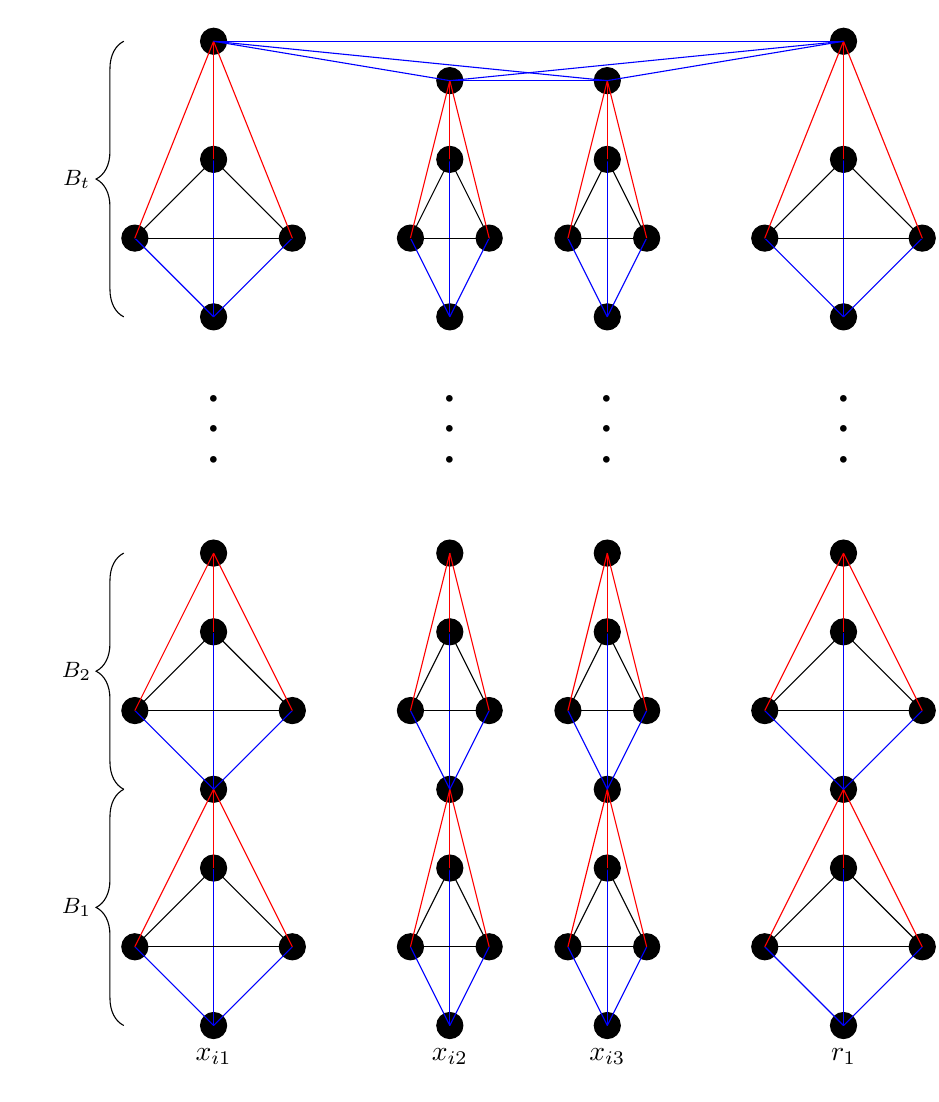
\begin{tikzpicture}
	  \node[circle,draw,minimum size=1mm,,fill=black,label=below:$x_{i1}$] at (0, 0){};
	  \node[circle,draw,fill=black] at (0, 2){};
	  \node[circle,draw,fill=black] at (-1, 1){};
	  \node[circle,draw,fill=black] at (1, 1){};
	  \node[circle,draw,fill=black] at (0, 3){};

	  \node[circle,draw,fill=black] at (0, 5){};
	  \node[circle,draw,fill=black] at (-1, 4){};
	  \node[circle,draw,fill=black] at (1, 4){};
	  \node[circle,draw,fill=black] at (0, 6){};
			
	  \node[circle,draw,fill=black] at (0, 9){};
	  \node[circle,draw,fill=black] at (0, 11){};
	  \node[circle,draw,fill=black] at (-1, 10){};
	  \node[circle,draw,fill=black] at (1, 10){};
	  \node[circle,draw,fill=black] at (0, 12.5){};
	
	  \draw[blue] (0, 0) -- (0, 2);
	  \draw[blue] (0, 0) -- (-1, 1);
	  \draw[blue] (0, 0) -- (1, 1);
	  \draw (1, 1) -- (-1, 1);
	  \draw (1, 1) -- (0, 2);
	  \draw (-1, 1) -- (0, 2);
	  \draw[red] (1, 1) -- (0, 3);
	  \draw[red] (-1, 1) -- (0, 3);
	  \draw[red] (0, 3) -- (0, 2);
		
	  \draw[blue] (0, 3) -- (0, 5);
	  \draw[blue] (0, 3) -- (-1, 4);
	  \draw[blue] (0, 3) -- (1, 4);
	  \draw (1, 4) -- (-1, 4);
	  \draw (1, 4) -- (0, 5);
	  \draw (-1, 4) -- (0, 5);
	  \draw[red] (1, 4) -- (0, 6);
	  \draw[red] (-1, 4) -- (0, 6);
	  \draw[red] (0, 6) -- (0, 5);
	
	  \draw[blue] (0, 9) -- (0, 11);
	  \draw[blue] (0, 9) -- (-1, 10);
	  \draw[blue] (0, 9) -- (1, 10);
	  \draw (1, 10) -- (-1, 10);
	  \draw (1, 10) -- (0, 11);
	  \draw (-1, 10) -- (0, 11);
	  \draw[red] (1, 10) -- (0, 12.5);
	  \draw[red] (-1, 10) -- (0, 12.5);
	  \draw[red] (0, 12.5) -- (0, 11);
	  	
	  \node[circle,draw,minimum size=1mm,,fill=black,label=below:$x_{i2}$] at (3, 0){};
	  \node[circle,draw,fill=black] at (3, 2){};
	  \node[circle,draw,fill=black] at (2.5, 1){};
	  \node[circle,draw,fill=black] at (3.5, 1){};
	  \node[circle,draw,fill=black] at (3, 3){};
	
	  \node[circle,draw,fill=black] at (3, 5){};
	  \node[circle,draw,fill=black] at (2.5, 4){};
	  \node[circle,draw,fill=black] at (3.5, 4){};
	  \node[circle,draw,fill=black] at (3, 6){};
		
	  \node[circle,draw,fill=black] at (3, 9){};
	  \node[circle,draw,fill=black] at (3, 11){};
	  \node[circle,draw,fill=black] at (2.5, 10){};
	  \node[circle,draw,fill=black] at (3.5, 10){};
	  \node[circle,draw,fill=black] at (3, 12){};
	  		
	  \draw[blue] (3, 0) -- (3, 2);
	  \draw[blue] (3, 0) -- (2.5, 1);
	  \draw[blue] (3, 0) -- (3.5, 1);
	  \draw (3.5, 1) -- (2.5, 1);
	  \draw (3.5, 1) -- (3, 2);
	  \draw (2.5, 1) -- (3, 2);
	  \draw[red] (2.5, 1) -- (3, 3);
	  \draw[red] (3.5, 1) -- (3, 3);
	  \draw[red] (3, 3) -- (3, 2);
	  
	  \draw[blue] (3, 3) -- (3, 5);
	  \draw[blue] (3, 3) -- (2.5, 4);
	  \draw[blue] (3, 3) -- (3.5, 4);
	  \draw (3.5, 4) -- (2.5, 4);
	  \draw (3.5, 4) -- (3, 5);
	  \draw (2.5, 4) -- (3, 5);
	  \draw[red] (3.5, 4) -- (3, 6);
	  \draw[red] (2.5, 4) -- (3, 6);
	  \draw[red] (3, 6) -- (3, 5);
	  
	  \draw[blue] (3, 9) -- (3, 11);
	  \draw[blue] (3, 9) -- (2.5, 10);
	  \draw[blue] (3, 9) -- (3.5, 10);
	  \draw (3.5, 10) -- (2.5, 10);
	  \draw (3.5, 10) -- (3, 11);
	  \draw (2.5, 10) -- (3, 11);
	  \draw[red] (3.5, 10) -- (3, 12);
	  \draw[red] (2.5, 10) -- (3, 12);
	  \draw[red] (3, 12) -- (3, 11);
	  
	  \node[circle,draw,minimum size=1mm,,fill=black,label=below:$x_{i3}$] at (5, 0){};
	  \node[circle,draw,fill=black] at (5, 2){};
	  \node[circle,draw,fill=black] at (4.5, 1){};
	  \node[circle,draw,fill=black] at (5.5, 1){};
	  \node[circle,draw,fill=black] at (5, 3){};
	
	  \node[circle,draw,fill=black] at (5, 5){};
	  \node[circle,draw,fill=black] at (4.5, 4){};
	  \node[circle,draw,fill=black] at (5.5, 4){};
	  \node[circle,draw,fill=black] at (5, 6){};
		
	  \node[circle,draw,fill=black] at (5, 9){};
	  \node[circle,draw,fill=black] at (5, 11){};
	  \node[circle,draw,fill=black] at (4.5, 10){};
	  \node[circle,draw,fill=black] at (5.5, 10){};
	  \node[circle,draw,fill=black] at (5, 12){};
	  		
	  \draw[blue] (5, 0) -- (5, 2);
	  \draw[blue] (5, 0) -- (4.5, 1);
	  \draw[blue] (5, 0) -- (5.5, 1);
	  \draw (5.5, 1) -- (4.5, 1);
	  \draw (5.5, 1) -- (5, 2);
	  \draw (4.5, 1) -- (5, 2);
	  \draw[red] (5.5, 1) -- (5, 3);
	  \draw[red] (4.5, 1) -- (5, 3);
	  \draw[red] (5, 3) -- (5, 2);
	  
	  \draw[blue] (5, 3) -- (5, 5);
	  \draw[blue] (5, 3) -- (4.5, 4);
	  \draw[blue] (5, 3) -- (5.5, 4);
	  \draw (5.5, 4) -- (4.5, 4);
	  \draw (5.5, 4) -- (5, 5);
	  \draw (4.5, 4) -- (5, 5);
	  \draw[red] (5.5, 4) -- (5, 6);
	  \draw[red] (4.5, 4) -- (5, 6);
	  \draw[red] (5, 6) -- (5, 5);
	  
	  \draw[blue] (5, 9) -- (5, 11);
	  \draw[blue] (5, 9) -- (4.5, 10);
	  \draw[blue] (5, 9) -- (5.5, 10);
	  \draw (5.5, 10) -- (4.5, 10);
	  \draw (5.5, 10) -- (5, 11);
	  \draw (4.5, 10) -- (5, 11);
	  \draw[red] (5.5, 10) -- (5, 12);
	  \draw[red] (4.5, 10) -- (5, 12);
	  \draw[red] (5, 12) -- (5, 11);
	  
	  \node[circle,draw,minimum size=1mm,label=below:$r_{1}$,fill=black] at (8, 0){};
	  \node[circle,draw,fill=black] at (8, 2){};
	  \node[circle,draw,fill=black] at (7, 1){};
	  \node[circle,draw,fill=black] at (9, 1){};
	  \node[circle,draw,fill=black] at (8, 3){};

	  \node[circle,draw,fill=black] at (8, 5){};
	  \node[circle,draw,fill=black] at (7, 4){};
	  \node[circle,draw,fill=black] at (9, 4){};
	  \node[circle,draw,fill=black] at (8, 6){};
			
	  \node[circle,draw,fill=black] at (8, 9){};
	  \node[circle,draw,fill=black] at (8, 11){};
	  \node[circle,draw,fill=black] at (7, 10){};
	  \node[circle,draw,fill=black] at (9, 10){};
	  \node[circle,draw,fill=black] at (8, 12.5){};
	
	  \draw[blue] (8, 0) -- (8, 2);
	  \draw[blue] (8, 0) -- (7, 1);
	  \draw[blue] (8, 0) -- (9, 1);
	  \draw (9, 1) -- (7, 1);
	  \draw (9, 1) -- (8, 2);
	  \draw (7, 1) -- (8, 2);
	  \draw[red] (9, 1) -- (8, 3);
	  \draw[red] (7, 1) -- (8, 3);
	  \draw[red] (8, 3) -- (8, 2);
		
	  \draw[blue] (8, 3) -- (8, 5);
	  \draw[blue] (8, 3) -- (7, 4);
	  \draw[blue] (8, 3) -- (9, 4);
	  \draw (9, 4) -- (7, 4);
	  \draw (9, 4) -- (8, 5);
	  \draw (7, 4) -- (8, 5);
	  \draw[red] (9, 4) -- (8, 6);
	  \draw[red] (7, 4) -- (8, 6);
	  \draw[red] (8, 6) -- (8, 5);
	
	  \draw[blue] (8, 9) -- (8, 11);
	  \draw[blue] (8, 9) -- (7, 10);
	  \draw[blue] (8, 9) -- (9, 10);
	  \draw (9, 10) -- (7, 10);
	  \draw (9, 10) -- (8, 11);
	  \draw (7, 10) -- (8, 11);
	  \draw[red] (9, 10) -- (8, 12.5);
	  \draw[red] (7, 10) -- (8, 12.5);
	  \draw[red] (8, 12.5) -- (8, 11);
	
	  \draw[blue] (0, 12.5) -- (8, 12.5);
	  \draw[blue] (0, 12.5) -- (5, 12);
	  \draw[blue] (0, 12.5) -- (3, 12);
	  \draw[blue] (3, 12) -- (5, 12);
	  \draw[blue] (3, 12) -- (8, 12.5);
	  \draw[blue] (5, 12) -- (8, 12.5);
	  
	  \path (0, 9) -- (0, 6) node [black, font=\Huge, midway, sloped] {$\dots$};
	  \path (3, 9) -- (3, 6) node [black, font=\Huge, midway, sloped] {$\dots$};
	  \path (5, 9) -- (5, 6) node [black, font=\Huge, midway, sloped] {$\dots$};
	  \path (8, 9) -- (8, 6) node [black, font=\Huge, midway, sloped] {$\dots$};
	  
	  \draw [decorate,decoration={brace,amplitude=10pt},xshift=-4pt,yshift=0pt]
(-1,0) -- (-1,3) node [black,midway,xshift=-0.6cm] 
{\footnotesize $B_1$};
	  \draw [decorate,decoration={brace,amplitude=10pt},xshift=-4pt,yshift=0pt]
(-1,3) -- (-1,6) node [black,midway,xshift=-0.6cm] 
{\footnotesize $B_2$};
	  \draw [decorate,decoration={brace,amplitude=10pt},xshift=-4pt,yshift=0pt]
(-1,9) -- (-1,12.5) node [black,midway,xshift=-0.6cm] 
{\footnotesize $B_t$};

	\end{tikzpicture}
\caption{Part of graph $G$ constructed for the subset $S_i =  \{x_{i1}, x_{i2}, x_{i3}\}$. The graph is constructed by local replacement when for $p = 4$. If $S_i$ is included in the exact cover then the edges colored black and the edges colored blue represent the corresponding clustering of this part of the graph $G$. If $S_i$ is not included in the exact cover then the edges colored red and the edges colored black represent the clustering of this part of the graph.}
\label{fig:X3CNPHard}
\end{figure*}

\begin{theorem}
Finding the optimal solution to the Promise Correlation Clustering problem is NP-Hard for all $M \ge 3$ and for $\alpha = 0$ and $\beta = \frac{1}{2}$.  
\end{theorem}

\noindent To prove the result, we will use a reduction from exact cover by $3$-sets problem which is known to be NP-Hard.

(X3C) Given a universe of elements $U = \{x_1, \ldots, x_{3q}\}$ and a collections of subsets $S = \{S_1, \ldots, S_m\}$. Each $S_i \subset U$ and contains exactly three elements. Does there exist $S' \subseteq S$ such that each element of $U$ occurs exactly once in $S'$?

This decision problem is known to be NP-Hard. We will now reduce an instance of X3C to the promise correlation clustering problem. For each three set $S_i = \{x_{i1}, x_{i2}, x_{i3}\}$, we construct a replacement gadget as described in Fig. \ref{fig:X3CNPHard}. The gadget is similar to the one used in the proof of partition into triangles problem. However, instead of triangles the graph is `made of' cliques of size $p$. 



Given an instance of X3C, we construct $G = (V, E)$ using local replacement described in Fig. \ref{fig:X3CNPHard}. Let $A$ be an algorithm which solves the promise problem described in Eqn. \ref{eqn:promiseCorrLoss}. Then, we can use this algorithm to decide exact cover by three sets as follows.

If $A$ outputs a clustering $C$ such that all the clusters have size exactly $p$ and $E_C$ makes no negative errors w.r.t $E$ (that is $\mu(E_C) = 0$) then output YES. Otherwise, output NO. Next, we will prove that this procedure decides X3C. 

Let there exists an exact cover for the X3C instance. Let $C$ be the clustering corresponding to the exact cover. That is, the edges colored blue and black correspond to this clustering and the corresponding vertices are in the same cluster (Fig. \ref{fig:X3CNPHard}). Note that this clustering makes no negative errors. Furthermore, each point is in a cluster of size exactly $p$. Thus, the positive error corresponding to any vertex is the degree of that vertex minus $p-1$. Since, the size of a cluster is atmost $p$, this is the minimum possible positive error for any vertex. Hence, any other clustering strictly makes more positive errors than $C$. 

It is easy to see from the construction that if $A$ finds a clustering which has no negative errors and all the clusters have size $p$, then this corresponds to exact cover of the X3C instance and hence we output YES. If this does not happen then there does not exist any exact cover for $(U, S)$. This is because if there was an exact cover then the corresponding clustering would satisfy our condition. Thus, $A$ decides X3C. Since, X3C is NP-Hard, no polynomial time algorithm $A$ exists unless $P = NP$.

In the construction, for each clause, we have $p^2 t + (p - 3)$ vertices and a vertex for each of the variables. Therefore, $|V| = m (p^2 t + (p-3)) + 3q$ and $|E| = pt({p \choose 2}+p-1) + {p \choose 2}$.  Consider a clustering $C$ which places all the $x_i$'s  and $r_i$'s in singleton clusters and places rest of the points in clusters of size $p$. For $t \ge 2$,
\begin{align*}
  \beta &= \frac{pt{p \choose 2}}{pt({p \choose 2}+p-1) + {p \choose 2}} = \frac{1}{1 + \frac{2}{p} + \frac{1}{pt}} > \frac{1}{2} \text{ and }\alpha = 0
\end{align*} 

\subsection{Hardness of PCC in the presence of an oracle}
\label{section:PCCNPHardOracle}
In the previous sections, we have shown that the PCC problem is NP-Hard without queries. It is trivial to see that by making $\beta |X|$ queries to the same-cluster oracle allows us to solve (in polynomial time) the Promise Correlation Clustering problem for all $M$ and $\alpha = 0$. In this section, we prove that the linear dependence on $n = |X|$ is tight. We prove that if the exponential time hypothesis (ETH) holds then any algorithm that runs in polynomial time makes atleast $\Omega(n)$ same-cluster queries.

\begin{theorem}
Given that the Exponential Time Hypothesis (ETH) holds then any algorithm for the Promise Correlation Clustering problem  that runs in polynomial time makes $\Omega(|X|)$ same-cluster queries for all $M \ge 3$ and for $\alpha = 0$ and $\beta = \frac{1}{2}$. 
\end{theorem}

\noindent Below, we give a proof sketch but a detailed proof is in the supplementary material. The exponential time hypothesis says that any solver for $3$-SAT runs in $2^{o(m)}$ time (where $m$ is the number of clauses in the $3$-SAT formula). We use a reduction from $3$-SAT to 3DM to X3C to show that the exact cover by 3-sets (X3C) problem also can't be solved in $2^{o(m)}$ time (if ETH holds). Then, using the reduction from the previous section implies that PCC also can't be solved in $2^{o(n)}$ time. Thus, any query based algorithm for PCC needs to make atleast $\Omega(n)$ queries where $n = |X|$ is the number of vertices in the graph. 

\begin{definition}[3-SAT].\\
Input: A boolean formulae $\phi$ in 3CNF with $n$ literals and $m$ clauses. Each clause has exactly three literals. \\
Output: YES if $\phi$ is satisfiable, NO otherwise. 
\end{definition}

\noindent\textbf{Exponential Time Hypothesis}\\
There does not exist an algorithm which decides 3-SAT  and runs in $2^{o(m)}$ time.

\noindent To prove that (X3C) is NP-Hard, the standard We will reduce 3-SAT to 3-dimensional matching problem. 3DM is already known to be NP-Hard. However, the standard reduction of 3-SAT to 3DM constructs a set with number of matchings in $\Theta(m^2 n^2)$. Hence, using the standard reduction, the exponential time hypothesis would imply there does not exist an algorithm for 3DM which runs in $\Omega(m^\frac{1}{4})$. Our reduction is based on the standard reduction. However, we make some clever optimizations especially in the way we encode the clauses. This improves the lower bound to $\Omega(m)$.

Using the above result, we immediately get an $\Omega(2^m)$ lower bound on the run-time of X3C. Now, using the same reduction of X3C to PCC as in Section \ref{subsection:PCCNPHard}, gives the same lower bound of $\Omega(n)$ on the running time of PCC. 

For the sake of contradiction, let us assume that there exists an algorithm which solves PCC in polynomial time by making $o(n)$ same-cluster queries ($n$ is the number of vertices). Then by simulating all possible answers for the oracle, we get a non-query algorithm which solves PCC in $2^{o(n)}$. Hence, no such query algorithm exists. 

\ifdefined\COMPLETE
\else
\end{document}
\fi
\ifdefined\COMPLETE
\else
\documentclass[12pt]{article}

\usepackage{amsmath,amsthm,mathtools}
\usepackage{graphicx}
\usepackage{algorithm2e}
\usepackage{thm-restate}
\usepackage{enumitem}

\usepackage{tikz}
\usetikzlibrary{shapes, calc, arrows, through, intersections, decorations.pathreplacing, patterns}
\usepackage[labelformat=simple]{subcaption}
\usepackage[export]{adjustbox}

\newtheorem{theorem}{Theorem}
\newtheorem{definition}[theorem]{Definition}
\newtheorem{thrm}[theorem]{Theorem}
\newtheorem{lem}[theorem]{Lemma}
\newtheorem{corollary}[theorem]{Corollary}

\newcommand{\mb}{\mathbf}
\newcommand{\mc}{\mathcal}
\newcommand\numberthis{\addtocounter{equation}{1}\tag{\theequation}}
\let\oldnl\nl
\newcommand{\nonl}{\renewcommand{\nl}{\let\nl\oldnl}}
\renewcommand\thesubfigure{(\alph{subfigure})}

\DeclareMathOperator*{\argmin}{arg\,min}
\DeclareMathOperator*{\vcdim}{VC-Dim}

\begin{document}
\fi

\section{Restricted Correlation Clustering}
\label{section:RCC}

The results in the previous section show that even under strong promise, correlation clustering is still NP-Hard. Furthermore, it is hard even when given access to an oracle. 

Observe that the requirement of correlation clustering is very demanding. The algorithm is required to find a clustering over the set of all possible clusterings of the domain $X$. In the restricted framework, we change the goalpost slightly. The algorithm is now required to find a clustering $C$ from a class $\mc F$ (of clusterings of $X$). 

\begin{definition}[Restricted correlation clustering (RCC)]
\label{defn:rcc}
Given a clustering instance $(X, d)$, an unknown target clustering $C^*$ and weighting parameter $\mu$. Given a finite class $\mc F$ of clusterings of the set $X$. Find $C \in \mc F$ such that 
\begin{align}
\hat C = \argmin_{C \in \mc F} \enspace L_{C^*}(C)\label{eqn:RCCMain}
\end{align}
\end{definition}

\subsection{Relation to practical applications}
Consider the following scenario from the practitioner's point of view. The practitioner wants to implement correlation clustering. However, he/she knows that the problem is NP-Hard. The practitioner has prior knowledge that one of the many hierarchical clustering algorithms (like single-linkage or max-linkage or average-linkage or complete-linkage) is suitable for his/her dataset\footnote{A nice overview of hierarchical clustering techniques can be found in \cite{maimon2009nhecd}}. A hierarchical clustering algorithm outputs a clustering tree. Every pruning of the tree is a clustering of the original dataset. He/she would now like to know which amongst these clustering algorithms is suitable for his task. After having fixed the algorithm, the practitioner would then  like to know which amongst these many prunings he/she should chose. 

The framework of restricted correlation clustering is applicable in such scenarios. When $\mc F = \{T\}$ where $T$ is a hierarchical clustering of $X$, the goal of RCC is to find the pruning from the tree $T$ which has minimum normalized correlation loss. When $\mc F = \{T_1, \ldots, T_s\}$ where each $T_i$ is a hierarchical clustering of $X$. Then the goal of RCC is to find a pruning with minimum loss amongst the prunings of all the $s$ trees. Note that finding the pruning of the tree is the same as choosing the stopping point criteria when running linkage-based algorithms. Hence, the framework can help us choose the right stopping point for a particular hierarchical clustering algorithm.

If $\mc F = \{C_1, \ldots, C_s\}$ where each $C_i$ is a clustering of the set $X$ then the goal is to find a clustering with minimum loss. Note that $\mc F$ can be any of the examples as defined above or a union of these or some other finite class. 
    
\subsection{Solution strategy}
In the RCC framework, we wish to minimize the loss which depends on the unknown target clustering $C^*$. However, in the absence of any information about $C^*$, there is no hope to find a clustering that minimizes $L_{C^*}$. Hence, to solve the RCC problem we allow the clustering (or learning) algorithm to make queries to a $C^*$-oracle. 
  
Our goal is to calculate quantities $L_{P^+}(C)$ and $L_{P^-}(C)$ (Defn. \ref{defn:normalizedCorrelationLoss}) for each of the clusterings $C \in \mc F$ and then choose the clustering with minimum loss. To calculate both these quantities exactly, for each pair of points in our dataset, we would need to know whether they belong to the same-cluster or different-cluster. In other words, we would need access to the complete ground truth clustering $C^*$. Thus, instead of calculating these two quantities exactly we want to estimate them from a small sample, sampled according to the distributions $P^+$ and $P^-$.  

One strategy to estimate $L_{P^+}(C)$ (and $L_{P^-}$) could be the following. Sample a set $S_+$ (and $S_-$) of pairs using the distribution $P^+$ (and $P^-$). Compute the fraction of mistakes made by each clustering $C$ on $S_+$ (and $S_-$). Using the standard results from vc-dimension theory (Thm. \ref{thm:uniformConvergence}), it is known that using this procedure we can estimate $L_{P^+}$ for each of the clusterings $C \in \mc F$. Similarly, we could also estimate $L_{P^-}$. Using the two estimates, we could then estimate the loss $L_{C^*}$ for each of the clusterings in our class and choose the clustering which has the smallest loss. 

The main problem in this approach is that the distributions $P^+$ and $P^-$ are unknown (as the target clustering $C^*$ is not known). In Section \ref{section:samplingRCC}, we discuss two approaches which (approximately) sample according to these distributions. Then in Section \ref{section:sampleAndQueryComplexity}, we show how these sampling procedures can be used to estimate $L_{C^*}$ for all the clusterings in our class $\mc F$.

\section{Sampling for RCC}
\label{section:samplingRCC}
We first describe the procedure $\mc P_0$ which samples according to $P^-$. Then we describe the procedure $\mc P_1$ which samples approximately according to the distribution $P^+$. 

\RestyleAlgo{ruled}
\SetAlgoNoLine
\LinesNumbered
\SetNlSkip{-0.4em}
\begin{algorithm}
\label{alg:weightedNegPairs}
\caption{Procedure $\mc P_0$ for negative pairs}

\Indp\KwIn{A set $X$ and a $C^*$-oracle.}
\KwOut{$(x, y)$ such that $C^*(x, y) = 0$}

\vspace{0.1in} 
\While{TRUE}{
  Sample $(x, y)$ using $U^2$\\
  \If {$ C^*(x, y) = 0$}{
  		Output $(x, y)$
	}
}
\end{algorithm}
The procedure samples a pair uniformly at random. Then using the oracle it checks if the sampled pair is negative and terminates if such a pair is found. If not then the process is repeated again. 

\begin{restatable}{lem}{weightedNegUniform}
\label{lemma:weightedNegUniform}
Given $X$ and a $C^*$-oracle. The procedure $\mc P_0$ samples a pair $(x, y)$ according to the distribution $P^-$.
\end{restatable}
\begin{proof}
The probability that a negative pair is sampled during a trial is $U^2(X^{[2]-}) =: q$. Fix a negative pair $(x, y)$ and let $U^2(x, y) = p$. Hence, the probability that the pair $(x, y)$ is sampled $= p + (1-q)p + (1-q)^2p + \ldots = p\sum_{i=0}^\infty (1-q)^i = \frac{p}{q} = \frac{U^2(x, y)}{U^2(X^{[2]-})} = P^-(x, y)$.
\end{proof}

\noindent Note that to sample one negative pair, procedure $\mc P_0$ might need to ask more than one same-cluster query. However, since our input $X$ is $\gamma$-skewed, we `expect' the number of `extra' queries to be `small'. 

\begin{restatable}{lem}{negQueries}
\label{lemma:negQueries}Given set $X$ and a $C^*$-oracle. Let $X$ be $\gamma$-skewed and Let $q$ be the number of same-cluster queries made by $\mc P_0$ to the $C^*$-oracle. Then, $\mb E[q] \le \frac{1}{1-\gamma}$.
\end{restatable}
\begin{proof}
Let $p$ denote the probability that a negative pair is sampled during an iteration. We know that $p \ge (1 - \gamma)$. Let $q$ be a random variable denoting the number of iterations (or trials) before a negative pair is sampled. Then, $q$ is a geometric random variable. $\mb E[q] = \frac{1}{p} \le \frac{1}{1-\gamma}$.
\end{proof}

Lemma \ref{lemma:negQueries} shows that for $\gamma < \frac{1}{2}$, to sample a negative pair, procedure $\mc P_0$ makes atmost two queries to the oracle in expectation. Moreover, the number of queries is tight around the mean. Note that this sampling strategy is not useful for positive pairs. This is because the fraction of positive pairs in the dataset is small. Hence, to sample a single positive pair we would need to make `many' same-cluster queries. 

\subsection{Sampling positive pairs for general metrics}
\label{section:samplingPositive}

\RestyleAlgo{ruled}
\SetAlgoNoLine
\LinesNumbered
\SetNlSkip{-0.4em}
\begin{algorithm}
\caption{Sampling procedure $\mc P_{11}$ for positive pairs (general metrics)}
\label{alg:weightedPosPairs}
\Indp\KwIn{A set $X$, a $C^*$-oracle and a parameter $\lambda$.}
\KwOut{One pair $(x, y) \in X^{[2]}$ such that $\mc C^*(x, y) = 1$}

\vspace{0.1in}\textbf{Pre-compute:} For all $x \in X$, compute $S_x := \{y: d(x, y) \le \lambda\}$.\\

\vspace{0.1in} \While{TRUE}{
Sample $x \in X$ with probability $\propto |S_x|$.\\
Sample $y$ uniformly at random from $S_x$. \\
\If {$\mc C^*(x, y) = 1$}{
	Output $(x, y)$.
	}
}	
\end{algorithm}


Given a clustering instance $(X, d)$. Assume that the metric $d$ is $(\alpha, \beta)$-informative w.r.t target $C^*$ and parameter $\lambda$. This means that `most' of the positive pairs are within distance $\lambda$. Our sampling strategy is to ``construct" a set $K = \{(x, y) \in X^2: d(x, y) \le \lambda\}$ and then sample uniformly from this set. We will prove that this procedure approximates $P^+$. 

The sampling algorithm is described in Alg. \ref{alg:weightedPosPairs}. In the pre-compute stage, for all points $x$ we construct its set of `neighbours' ($S_x$). We then choose a point with probability proportional to the size of its neighbour-set and then choose the second point uniformly at random from amongst its neighbours. This guarantees that we sample uniformly from the set $K$.  



\begin{restatable}{thrm}{posDistribution}
\label{thm:posDistribution}
Given set $(X, d)$, a $C^*$-oracle and parameter $\lambda$. Let $d$ be $(\alpha, \beta)$-informative w.r.t $\lambda$ and $C^*$.  Then the sampling procedure $\mc P_{11}$ induces a distribution $T$ over $X^{[2]}$ such that for any labelling function $h$ over $X^{[2]}$ we have that $$\Big|\underset{(x, y) \sim P^+}{\mb P}\enspace \big[ h(x, y) = 0 ] - \underset{(x, y) \sim T}{\mb P}\enspace \big[ h(x, y) = 0 ]\Big|  \enspace \le \enspace 2\alpha.$$ 
\end{restatable}


\noindent Note that to sample one positive pair, procedure $\mc P_{11}$ might need to ask more than one same-cluster query. However, since the metric $d$ is $\beta$-informative, we `expect' the number of `extra' queries to be `small'. 

\begin{restatable}{lem}{posQueries}
\label{lemma:posQueries}
Given set $(X, d)$, a $C^*$-oracle and a parameter $\lambda$. Let $d$ be $\beta$-informative w.r.t $\lambda$ and let $q$ be the number of same-cluster queries made by $\mc P_{11}$ to the $C^*$-oracle. Then, $\mb E[q] \le \frac{1}{\beta}$.
\end{restatable}
\begin{proof}
Let $p$ denote the probability that a positive pair is sampled during an iteration. We know that $p \ge \beta$. Let $q$ be a random variable denoting the number of iterations (or trials) before a positive pair is sampled. Then, $q$ is a geometric random variable. $\mb E[q] = \frac{1}{p} \le \frac{1}{\beta}$.
\end{proof}

\subsection{Sampling positive pairs for LSHable metrics}
\label{section:samplingPositiveLSHable}

The strategy in the previous section was to construct a set $K = \{(x, y): d(x, y) \le \lambda\}$ and then sample uniformly from the set $K$ till a positive sample is found. Since most of the positive pairs have distance $\le \lambda$, this sampling procedure approximates $P^+$ (the uniform distribution over the set of true positives). However, constructing the set $K$ requires $\Theta(|X|^2)$ time. In this section, we show that if the metric $d$ has some additional structure (is hashable) then we can reduce the pre-processing time to $O(|X|)$. We develop a sampling procedure $\mc P_{12}$ using techniques from locality sensitive hashing (LSH) combined with rejection sampling. We will show that $\mc P_{12}$ needs only linear pre-processing time (to build the hash maps) and outputs a positive pair sampled approximately according to $P^+$.\\

\noindent\textit{Locality Sensitive Hashing (LSH)}

\vspace{0.02in}\noindent Before we describe our technique, we introduce some relevant notation. A hash function $h: X \rightarrow \mb N$ maps the set $X$ onto the set of natural numbers. Thus, a hashing function partitions the input of size $n$ into $m \le n$ different buckets (or blocks) $B_1, \ldots, B_m$ where each $B_i = \{x : h(x) = b_i\}$ for some $b_i$. Given $(X, d)$, a Locality Sensitive Hashing (LSH) scheme w.r.t the distance metric $d$ (or a similarity metric) aims to partition $X$ into buckets such that `similar' items map to the same bucket with high probability and `dissimilar' items end up in different buckets with high probability. For example, MinHash scheme w.r.t Jaccard similarity measure \cite{broder2000min, broder1997resemblance} is a common LSH-based hashing scheme. Another example is SimHash scheme w.r.t hamming similarity measure \cite{charikar2002similarity}. 


\begin{definition}[LSH-based hashing algorithm]
\label{defn:LSHProperty}
Given a set $(X, d)$ and parameter $s$. An LSH-based hashing algorithm (or scheme) $\mc A$ outputs $s$ different partitions $P_1, \ldots, P_s$ of $X$. Denote $P_i = \{B_{i1}, \ldots, B_{in_i}\}$. We say that $\mc A$ is $(\epsilon, \epsilon')$-tight w.r.t $d$ and $\lambda, \lambda'$ if 

\begin{itemize}
	\item If $d(x, y) \le \lambda$ then  ${\mb P} [ b(x, y) = 1 ]  >  1 - \epsilon$
	\item If $d(x, y) > \lambda'$ then ${\mb P} [ b(x, y) = 1 ] < \epsilon'$
\end{itemize}
where $b(x, y) = 1$ if and only if $x, y$ are together in atleast one of the blocks $B_{ij}$.

Infact, we show that by choosing $s$ (and other parameters) appropriately, we can construct LSH schemes which are $(\epsilon, \epsilon'=s\ln (1+\epsilon))$-tight w.r.t $\lambda$ and $\lambda' = 2\lambda \ln (1+1/\epsilon)$. Thus, for simplicity of notation, we say that $\mc A$ is $\epsilon$-tight w.r.t $\lambda$ to mean that it is $(\epsilon, \epsilon')$-tight w.r.t $\lambda, \lambda'$ as chosen above.
\end{definition}

\noindent Throughout the remainder of this section, we will assume that the hashing scheme satisfies $\epsilon$-tightness. In the appendix, we provide details about why this assumption is justified. However, these results are orthogonal to the current discussion. Hence, we omit it here and only include it in the appendix (Thm. \ref{thm:similarInSame}).  

We now describe our sampling procedure. Let $\mc B := \{P_1, \ldots, P_s\} = \{B_{ij} : 1\le i\le s, 1\le j \le |P_i|\}$ be the set of blocks outputted by the hashing scheme and let $Q := \{(x, y) \in B_{ij}\}$.  We first choose a block $B \in \mc B$ with probability proportional to $|B|^2$ (the number of pairs in the block). Then we sample a pair uniformly at random from this block $B$. Note that this strategy doesn't give us a uniform sample from $Q$. This is because a pair $(x, y)$ may be present in multiple blocks. To get the uniform sample, we reject the pair with probability inversely proportional to $a(x, y)$ (the number of blocks in which $x, y$ are together). This approach based on rejection sampling ensures that we have a uniform sample from $Q$. 

Next, we check if the pair satisfies $d(x, y) \le \lambda$. Note that the LSH-based scheme tries to put similar points in the same bucket, hence the probability of success at this step is `high'. Finally, we check if $C^*(x, y) = 1$. Our sampling procedure $\mc P_{1}$ is described in Alg. \ref{alg:weightedPosPairsHash}. 

\begin{algorithm}[h]
\caption{Sampling procedure $\mc P_{12}$ for positive pairs}
\Indp\KwIn{A set $\mc X$, a hashing algorithm $\mc A$, a $C^*$-oracle and parameter $\lambda$.}
\KwOut{$(x, y)$ such that $ C^*(x, y) = 1$}

\vspace{0.1in}\nonl\textbf{Pre-compute:} \\
	Use an LSH-based hashing scheme $\mc A$ to obtain partitions $\{P_1, \ldots, P_s\}$.\\
	$\mc B := \{P_1, \ldots, P_s\} = \{B_{ij} : 1\le i\le s, 1\le j \le |P_i|\}$.\\

\setcounter{AlgoLine}{0}

\vspace{0.1in}\nonl\textbf{Sampling:} \\
\While{TRUE}{
	Sample a block $B$ from $\mc B$ with probability $\propto |B|^2$.\\
	Sample $(x, y)$ uniformly at random from $B^2$. \\
	Let $a(x, y) = \{(x, y) \in B^2: B \in \mc B\}$. \\
	Sample $u$ uniformly at random from $[0, 1]$.\\
		\If{$u > \frac{1}{|a(x, y)|}$}{ \label{algLine:uCheck}
			\textbf{continue}.
		}
	\If {$d(x, y) \le \lambda$ and $C^*(x, y) = 1$ } {\label{algLine:oracleP22}
			 Output $(x, y)$.
	 }	
}
\label{alg:weightedPosPairsHash}
\end{algorithm}


Thm. \ref{thm:posDistributionLSH} shows that with high probability the procedure $\mc P_{12}$ samples a pair according to a distribution $\mc T$  which approximates $P^+$. 
\begin{restatable}{thrm}{posDistributionLSH}
\label{thm:posDistributionLSH}
Given $(X, d)$, a $C^*$-oracle and parameter $\lambda$. Let $d$ satisfy $(\alpha, \beta)$-informative  w.r.t $C^*$. Let the hashing algorithm $\mc A$ satisfy $\epsilon$-tightness w.r.t $\lambda$. Then with probability atleast $1-\exp(-2(\nu(1-\alpha)|X^2_+|)^2)$ (over the randomness in the hashing algorithm), $\mc P_{12}$ samples pairs $(x, y)$  according to distribution $\mc T$ over $X^{[2]}$ such that for any labelling function $C : X^{[2]} \rightarrow \{0, 1\}$, we have that 
\begin{align*}
  &\underset{(x, y) \sim P^+}{\mb P} \big[ C(x, y) = 0 ] -\alpha -\epsilon -\nu \le \underset{(x, y) \sim T}{\mb P} \big[ C(x, y) = 0 ] \\
  &\le  (1 + 2\nu)(1+2\alpha) \underset{(x, y) \sim P^+}{\mb P} \big[ C(x, y) = 0 ]
\end{align*} 
\end{restatable}

To sample one same-cluster pair, we might need to make more than one same-cluster query to the $C^*$-oracle. Lemma \ref{lemma:posQueriesLSH} shows that with high probability, the number of queries made by $\mc P_{12}$ to sample one positive pair is upper bounded by a small constant. 

\begin{restatable}{lem}{posQueriesLSH}
\label{lemma:posQueriesLSH}
Given set $X$, a $C^*$-oracle and parameter $\lambda$. Let $d$ be $(\alpha, \beta)$-informative w.r.t $\lambda$ and $C^*$. Let $\mc A$ satisfy $\epsilon$-tightness w.r.t $\lambda$. Let $q$ be the number of same-cluster queries made by $\mc P_{12}$. Then with probability atleast $1-\exp(-\nu^2(1-\alpha)^2|X^2_+|^2)$ (over the randomness in the hashing algorithm) $$\mb E[q] \le \frac{1}{\beta(1-\epsilon-\nu)}$$ 
\end{restatable}

The pre-compute stage uses a hashing algorithm to obtain $s$ different partitions. From the discussion in the appendix (Thm. \ref{thm:hashTimeComplexity}), we its easy to see that this runs in $O(n)$ time. Next, we  analyse the time taken to sample one same-cluster pair.  Thm. \ref{thm:posRuntimeLSH} shows that under reasonable assumptions, the time taken is upper bounded by a constant with high probability. 

\begin{restatable}{thrm}{posRuntimeLSH}
\label{thm:posRuntimeLSH}
Given set $X$, a $C^*$-oracle and parameter $\lambda$. Let $d$ be $(\alpha, \beta)$-informative w.r.t $\lambda$ and $C^*$. Let $\mc A$ satisfy $\epsilon$-tightness w.r.t $\lambda$. 

Define $\lambda' = 2\lambda\log(1+\frac{1}{\epsilon})$ and $\epsilon' = \lceil \log(\frac{1}{\epsilon})\rceil (1+\log(\frac{1}{\epsilon}))$. Let $K = \{(x, y) : d(x, y) \le \lambda\}$ is the set of all pairs of points with distance $\le \lambda$. Similarly, define sets $K_1 = \{(x, y): \lambda < d(x, y) \le \lambda'\}$ and $K_2 = \{(x, y): d(x, y) > \lambda'\}$. Let $|K_1| \le \rho_1|K|$ and $\epsilon'|K_2| \le \rho_2|K|$. 

Let $t$ be the time taken to sample one point by procedure $\mc P_{12}$. Then with probability atleast $1- \exp\Big(\frac{-\nu^2(1-\epsilon)(1-\alpha)|X^2_+|}{2}\Big)- \exp\Big(\frac{-\nu^2\rho_2 |K|}{3}\Big)$ (over the randomness in the hashing algorithm), we have that $$\mb E[t] \le s^2(1+\frac{1}{\eta})$$
where $\eta := \frac{(1-\nu)(1-\epsilon)\beta}{(1+\nu)(1+\rho_1+\rho_2)}$. 
\end{restatable}


\section{Sample and query complexity of RCC}
\label{section:sampleAndQueryComplexity}
In the previous section we saw how to sample (approximately) according to the distributions $P^+$ and $P^-$. We sample a `small' set of true positive (or same-cluster) and true negative (or different-cluster) pairs using our distributions. We then choose the clustering $\hat C \in \mc F$ with the minimum number of mistakes on the sampled pairs. We prove that the true normalized correlation loss $L_{C^*}(C)$ is close to the loss of $\hat C^*$ (the clustering with minimum loss in $\mc F$). Thus, our solution strategy shows that by only having a small amount of information about $C^*$ (making a small number of queries) we can find a clustering which is close (in terms of loss) to the optimal clustering in $\mc F$. We describe this procedure in Alg. \ref{alg:ERM}. 

Note that in this section, we have assumed that procedure $\mc P_{11}$ is used for sampling positive pairs. Similar results can be obtained when instead procedure $\mc P_{12}$ is used for sampling positive pairs. However, we include those results only in the appendix. 

\RestyleAlgo{ruled}
\SetAlgoNoLine
\LinesNumbered
\SetNlSkip{-0.4em}
\begin{algorithm}[h]
\caption{Empirical Risk Minimization}
\label{alg:ERM}
\Indp\KwIn{$( X, d)$, a set of clusterings $\mc F$, a $C^*$-oracle, parameter $\lambda$ and sizes $m_+$ and $m_-$.}
\KwOut{$ C \in \mc F$}

\vspace{0.1in} 
Sample a sets $S_+$ and $S_-$ of sizes $m_+$ and $m_-$ using procedures $\mc P_{11}$ and $\mc P_0$ respectively.\\
For every $C \in \mc F$, compute
\vspace{-0.1in}\begin{align*}
  &\hat P(C) = \frac{|\{(x, y) \in S_+: C(x, y) = 0\}|}{|S_+|}\\
  &\hat N(C) = \frac{|\{(x, y) \in S_-: C(x, y) = 0\}|}{|S_-|}
\end{align*}

Define $\hat L(C) = \mu \hat P(C) + (1-\mu)\hat N(C)$. \label{algLine:alpha}\\
Output $\argmin_{C \in \mc F} \enspace \hat L(C)$ \label{algLine:ERM}
\end{algorithm}

Thm. \ref{thm:sampleComplexity} analyses the sample complexity of our approach. That is, the number of labelled positive and negative pairs our algorithm needs as input, so that the estimates of the loss based on this sample are close to their true values. We show that as long as the number of sampled pairs are in $O(\frac{\vcdim(\mc F)}{\epsilon^2})$ then our algorithm finds a clustering $\hat C$ which is close to the best clustering in $\mc F$. Here, $\vcdim$ is a combinatorial property which measures how `complex' or rich the class of clusterings is. Note that the number of samples needed is independent of the size of the dataset $X$. 

For common classes, like $\mc F = \{T_1, \ldots, T_s\}$ where each $T_i$ is a hierarchical clustering of $X$, we also analyze their $\vcdim(\mc F)$ and prove that it is in $o(\log^2 s)$. Thus for such classes a small number of samples suffice to find a clustering which is close to the best clustering in $\mc F$.  

\begin{restatable}{thrm}{sampleComplexity}
\label{thm:sampleComplexity}
Given metric space $(X, d)$, a class of clusterings $\mc F$ and a threshold parameter $\lambda$. Given $\epsilon, \delta \in (0, 1)$ and a $C^*$-oracle. Let $d$ be $(\alpha, \beta)$-informative and $X$ be $\gamma$-skewed w.r.t $\lambda$ and $C^*$. Let $\mc A$ be the ERM-based approach as described in Alg. \ref{alg:ERM} and $\hat C$ be the output of $\mc A$. If  
\begin{align}
  &m_-, m_+ \enspace \ge a\frac{\vcdim({\mc F}) + \log(\frac{2}{\delta})}{\epsilon^2} 
\end{align}
where $a$ is a global constant then with probability atleast $1-\delta$ (over the randomness in the sampling procedure), we have that $$L_{C^*}(\hat C) \enspace\le\enspace \min_{\mc C \in \mc F} L_{C^*}(\mc C) + 3\alpha + \epsilon$$
\end{restatable}
\begin{proof}
Let $T_0$ be the distribution induced by $\mc P_0$ and $T_1$ be the distribution induced by $\mc P_{11}$. Denote by $E(h) = \underset{(x, y) \sim P^+}{\mb P}\enspace \big[ h(x, y) = 0 ]$ and by $G(h) = \underset{(x, y) \sim P^-}{\mb P}\enspace \big[ h(x, y) = 1 ]$. 

Using Thm. \ref{thm:uniformConvergence}, we know that if $m_+ > a\frac{\vcdim({\mc F}) + \log(\frac{1}{\delta})}{\epsilon^2}$ then with probability atleast $1-\delta$, we have that for all $h$
\begin{align*}
  &|\hat E(h) - \underset{(x,y) \sim T_1}{\mb P}[h(x, y) = 0]| \le \epsilon\\
  \implies &\hat E(h) \le \epsilon + \underset{(x,y) \sim T_1}{\mb P}[h(x, y) = 0] \le \epsilon + 2\alpha + E(h) \enspace\text{ and}\\
  &E(h) - 2\alpha -\epsilon \le \hat E(h) \numberthis \label{eqn:eHat}
\end{align*}
Note that we obtain upper and lower bounds for $\underset{(x,y) \sim T_1}{\mb P}[h(x, y) = 0]$ using Thm. \ref{thm:posDistribution}. Similarly, if $m_- > a\frac{\vcdim({\mc F}) + \log(\frac{1}{\delta})}{\epsilon^2}$, then with probability atleast $1-\delta$, we have that for all $h$,
\begin{align*}
  &|\hat G(h) - \underset{(x,y) \sim T_0}{\mb P}[h(x, y) = 1]| \le \epsilon\\
  \implies &\hat G(h) \le \epsilon + G(h) \enspace\text{ and } \enspace G(h) -\epsilon \le \hat G(h) \numberthis\label{eqn:gHat}
\end{align*}

\noindent Combining Eqns. \ref{eqn:eHat} and \ref{eqn:gHat}, we get that with probability atleast $1-2\delta$, we have that for all $C \in {\mc F}$
\begin{align*}
  &\hat L(C) \le \mu [\epsilon + E(h) + 2\alpha] + (1-\mu)(\epsilon + G(h)) \\
  &\le L(h) + \epsilon + 2\alpha\\
  &\text{And} \enspace \hat L(C) \ge \mu(E(h) -\epsilon - \alpha) + (1-\mu)(G(h) - \epsilon) \\
  &\ge L(h) - \epsilon - \alpha
\end{align*}
Now, let $\hat C$ be the output of $\mc A$ and let $\hat C^*$ be $\argmin_{C \in {\mc F}} L(C)$. Then, we have that with probability atleast $1-2\delta$
\begin{align*}
  L(\hat C) &\le \hat L(\hat C) + \alpha + \epsilon \le \hat L(\hat C^*) + \alpha + \epsilon \le L(\hat C^*) + 2\epsilon + 3\alpha 
\end{align*}

Choosing $\epsilon = \frac{\epsilon}{2}$ and $\delta = \frac{\delta}{2}$ throughout gives the result of the theorem.
\end{proof}

Finally, we analyse the query complexity of our approach. That is the number of queries that our algorithm makes to the $C^*$-oracle. Our algorithm makes queries during the sampling procedure. We see that to sample $m_-$ negative and $m_+$ positive pairs the number of queries is `close' to $m_+ + m_-$ with very high probability. Thus, the number of `wasted' queries is small.  

\begin{restatable}{thrm}{queryComplexity}[Query Complexity]
\label{thm:queryComplexity}
Let the framework be as in Thm. \ref{thm:sampleComplexity}. With probability atleast $1-\exp\big(-\frac{\nu^2m_-}{4}) - \exp\big(-\frac{\nu^2m_+}{4}\big)$ over the randomness in the sampling procedure, the number of same-cluster queries $q$ made by $\mc A$ is  
$$q \le (1+\nu)\bigg(\frac{m_-}{(1-\gamma)} + \frac{m_+}{\beta}\bigg)$$
\end{restatable}
\begin{proof}
Let $q_+$ denote the number queries to sample the set $S_+$. We know that $\mb E[q_+] \le \frac{1}{\beta}$. Given that the expectation is bounded as above, using Thm. \ref{thm:geometricRV}, we get that $q_+ \le \frac{(1+\nu)m_+}{\beta}$ with probability atleast $1-\exp(\frac{-\nu^2m_+}{4})$. Similarly, we get that with probability atleast $1-\exp(\frac{-\nu^2m_-}{4})$, $q_- \le \frac{(1+\nu)m_-}{(1-\gamma)}$.
\end{proof}

\subsection{VC-Dimension of some common classes of clusterings}
In the previous section, we proved that the sample complexity of learning a class of clusterings $\mc F$ depends upon $\vcdim({\mc F})$. Recall that ${\mc F}$ is the class of labellings induced by the clusterings in $\mc F$. In this section, we prove upper bounds on the VC-Dimension for some common class of clusterings. 

\begin{restatable}{thrm}{VCDim}
Given a finite set $\mc X$ and a finite class $\mc F = \{C_1, \ldots, C_s\}$ of clusterings of $\mc X$.
$$\vcdim({\mc F}) \le g(s)$$ where $g(s)$ is the smallest integer $n$ such that $B_{\sqrt n} \ge s$ where $B_i$ is the $i^{th}$ bell number \cite{bell2010number}. 
\end{restatable}


\noindent Note that $B_{\sqrt n} \in o(2^{n})$. Thus, the $\vcdim$ of a list of clusterings is in $o( \log s)$. Next, we discuss another common class of clusterings, namely hierarchical clustering trees. 

\begin{definition}[Hierarchical clustering tree]
Given a set $X$. A hierarchical clustering tree $T$ is a rooted binary tree with the elements of $X$ as the leaves. 
\end{definition}

\noindent Every pruning of a hierarchical clustering tree is a clustering of the set $X$. A clustering tree contains exponentially many (in the size of $\mc X$) clusterings. Given $\mc F = \{T_1, \ldots, T_s\}$ consists of $s$ different hierarchical clustering trees, the following theorem bounds the VC-Dimension of ${\mc F}$.

\begin{restatable}{thrm}{VCDimT}
Given a finite set $\mc X$ and a finite class $\mc F = \{T_1, \ldots, T_s\}$ where each $T_i$ is a hierarchical clustering over $\mc X$. Then 
$$\vcdim({\mc F}) \le g(s)$$ where $g(s)$ is the smallest integer $n$ such that $\frac{\sqrt n!}{\lfloor \sqrt n/2 \rfloor! \enspace 2^{\lfloor \sqrt n/2 \rfloor}} \ge s $
\end{restatable}


\section{Computation complexity of RCC for common clustering classes}
\label{section:efficientERM}

\RestyleAlgo{ruled}
\SetAlgoNoLine
\LinesNumbered
\SetNlSkip{-0.4em}
\begin{algorithm}[h]
\caption{ERM approach for a hierarchical clustering tree}
\label{alg:ERMTrees}
\Indp\KwIn{A set $X$, a set $ S \subseteq X^2$ labelled according to $C^*$. Given a clustering tree $T$ on $S_u = \{x: (x, y) \text{ or }  (y, x) \in S\}$.}
\KwOut{A clustering $\hat C \in T$ which implements ERM over $T$.}

\vspace{0.1in} Initialize $e(\nu) = a(\nu) = 0$ for all the leaf nodes $\nu$. \\
\For{all non-leaf nodes $\nu$ (in a bottom-up manner)}{\label{algLine:forNode}
Let $\nu_l$ be left sub-tree and $\nu_r$ the right sub-tree.\\
Initialize $s_a = d_a = 0$.\\
	\For{$(x, y) \in S$}{
	  \If {$x, y \in nl(\nu)$ and $C^*(x, y) = 0$}{
	      $d_a = d_a + 1$.
	  }
	  \If {$!(x \in nl(\nu_l)$ and $ y \in nl(\nu_r))$ and $!(y \in nl(\nu_l)$ and $ x \in nl(\nu_r))$}{\label{algLine:IfCondn}
		\textbf{continue}
	}
	\If {$C^*(x, y) = 1$}{
		$s_a = s_a + 1$.
	}
}
$a(\nu) = d_a$ \label{algLine:all}\\
$e(\nu) = \min \{e(\nu_l)+e(\nu_r)+s_a, a(\nu)\}$ \label{algLine:best}
}
\end{algorithm}

Alg. \ref{alg:ERM} described the general ERM approach to find the `best' clustering for any class $\mc F$ of clusterings. Consider the case when $\mc F = \{C_1, \ldots, C_s\}$ (a finite list of clusterings). Then to implement Alg. \ref{alg:ERM}, we first sample a set $S \subseteq X^2$ and then compute the error of each clustering on this set $S$. Computing the error of a clustering on $S$ takes $\Theta(|S|)$ time. Hence, for finite $\mc F$, the ERM approach can be implemented in time $\Theta(|\mc F| |S|)$. 

Now, let's focus on the case when $\mc F = \{T_1, \ldots, T_s\}$ (a finite set of clustering trees). Each tree $T_i$ can contain exponentially many clusterings. Hence, it is not clear if we can still implement the ERM approach in polynomial-time. Consider the problem of implementing the ERM approach when $\mc F = \{T\}$. The goal is to find the pruning in the tree which minimizes the loss $\hat L$. Given tree $T$, the clustering with the smallest loss is either the clustering which assigns all the points to a single cluster or the clustering with the best loss in $T_l$ (left subtree) concatenated with the clustering with the best loss in $T_r$ (right subtree). Before we describe our approach lets introduce a bit of notation.

For every node $\nu$ in the hierarchical clustering tree, let $nl(\nu)$ be the leaves which are descendants of $\nu$. For a leaf node $\nu$, $nl(\nu) = \{\nu\}$. Let $\mu_1 = \mu|S_-|$ and $\mu_2 = (1-\mu)|S_+|$. Let $$e(\nu) = \argmin_{C \in T_{\nu}} \mu_1|S_+|\hat P(C) + \mu_2|S_-|\hat N(C)$$ where $T_{\nu}$ is the tree $T$ restricted to the descendants of $\nu$. Let $a(\nu) = \mu_1|S_+|\hat P(C) + \mu_2|S_-|\hat N(C)$ where $C$ is the clustering which assigns all the descendants of $\nu$ to a single cluster. We are now ready tp describe our bottom-up approach in Alg. \ref{alg:ERMTrees}. Its easy to see that the running time of the approach is $\Theta(|S|^2)$. 

\section{Experimental evaluation}
\label{sec:evaluation}

\begin{table*}[t]
\centering
\resizebox{\textwidth}{!}{
\begin{tabular}{ |c || c|c||c|c|| c|c || c|c || c|c| } 
 \hline
  & \multicolumn{2}{c||}{\textbf{simulated}} & \multicolumn{2}{|c|}{\textbf{publications}} & \multicolumn{2}{c||}{\textbf{products I}} & \multicolumn{2}{c||}{\textbf{products II}} & \multicolumn{2}{c||}{\textbf{restaurants}}\\ \hline
Clustering & true loss & estimated loss & true loss & estimated loss & true loss & estimated loss & true loss & estimated loss & true loss & estimated loss \\ \hline
ArtPt           & 0.091         & 0.105         & 0.023         & 0.005         & 0.206         & 0.170         & 0.153         &   0.160           & 0.094	                        & 0.110 \\ \hline
Star            & 0.052         & 0.060         & 0.100         & 0.050         & 0.207	        & 0.190         & 0.231         &	0.170           & 0.041	                        & 0.045 \\ \hline
ApproxCorr      &  NA\footnote{ Algorithm did not finish within a reasonable time limit because of the high computational cost.}           & NA       & 0.180	        & 0.145         & 0.380	        & 0.310         & 0.373         &	0.340           & 0.094	                        & 0.065 \\ \hline
Markov          & 0.011         & \textbf{0.000}& 0.017	        & 0.010         & 0.159         & 0.130         & 0.125         &	0.085           & 0.045                         & 0.030 \\ \hline
Na\"iveDedup    & 0.397         & 0.365         & 0.497         & 0.495         & 0.413         & 0.405         & 0.394         &	0.380           & 0.094                         & 0.080 \\ \hline
C1 (single)     & 0.019         & 0.025	        & 0.016         & 0.018         & 0.150         & 0.110         & 0.131         &	0.120           & 0.022                         & \textbf{0.015} \\ \hline
C2 (complete)   & 0.005         & 0.005	        & 0.009	        & 0.009         & 0.150	        & 0.130	        & 0.135         &	0.065           & 0.034	                        & 0.040 \\ \hline
C3 (weighted)   & 0.002         & \textbf{0.000}& \textbf{0.005}& \textbf{0.006}& \textbf{0.110}& 0.110	        & 0.107         &	0.070           & \textbf{0.019}      & 0.020 \\ \hline
C4 (average)    & \textbf{0.001}& \textbf{0.000}& 0.007 	    & 0.017         & 0.120	        & \textbf{0.100}& \textbf{0.099}&	\textbf{0.060}  & \textbf{0.019}      & 0.020 \\ \hline \hline
Mean loss difference   &               & 0.016         &               & 0.014         &               & 0.027         &               &   0.035           &                        & 0.010 \\ \hline
\end{tabular}
}
\caption{True loss and the loss estimated by our framework.}
\label{tab:exp3}
\end{table*}

\begin{table}[t]
\centering
\resizebox{\textwidth}{!}{

\begin{tabular}{ |c|c|c|c|c|c|c|c|c| } 
\hline
  &  & \multicolumn{2}{|c|}{\textbf{25, 25 samples}} & \multicolumn{2}{|c|}{\textbf{100, 100 samples}} & \multicolumn{2}{|c|}{\textbf{500, 500 samples}} \\ \hline
Clustering & true loss & \# queries & estimated loss & \# queries & estimated loss & \# queries & estimated loss \\ \hline
C1 (single) & \textbf{0.06107}   &  51 & 0.06 & 204	&   0.025 & 1023 &	0.024   \\ \hline
C2 (complete) &	\textbf{0.04177} &	50 & 0.02 &	210 &	0.005 & 1024 &	0.016 \\ \hline
C3 (weighted) & \textbf{0.03831} &	50 & 0.02 &	203 &	0.015 &	1027 &	0.016 \\ \hline
C4 (average) &	\textbf{0.03489} &	52 & 0.02 &	207 &	0.020 &	1043 &	0.013 \\ \hline
\end{tabular}

}
\caption{Simulated dataset: Impact of number of samples on the loss of the clustering}
\label{tab:exp1}
\end{table}




\begin{table}[t]
\centering
\resizebox{\textwidth}{!}{

\begin{tabular}{ |c|c|c|c|c|c|c|c|c| } 
 \hline
  &  & \multicolumn{2}{|c|}{\textbf{25, 25 samples}} & \multicolumn{2}{|c|}{\textbf{100, 100 samples}} &  \multicolumn{2}{|c|}{\textbf{500, 500 samples}} \\ \hline
Clustering & true loss & \# queries & estimated loss & \# queries & estimated loss & \# queries & estimated loss \\ \hline
C1 (single) & \textbf{0.11075}   &  51 & 0.08 & 208 &	0.055 &	1031 &	0.041 \\ \hline
C2 (complete) &	\textbf{0.37172} &	50 & 0.34 &	204 &	0.315 &	1035 &	0.334 \\ \hline
C3 (weighted) & \textbf{0.29622} &	51 & 0.14 &	203 &	0.260 &	1037 &	0.239 \\ \hline
C4 (average) &	\textbf{0.26877} &	50 & 0.20 &	204 &	0.195 &	1027 &	0.202 \\ \hline
\end{tabular}

}

\caption{Publications dataset: Impact of number of samples on the loss of the clustering}
\label{tab:exp2}
\end{table}

\begin{figure}[t]
    \centering
    \begin{subfigure}[t]{0.5\textwidth}
        \centering
        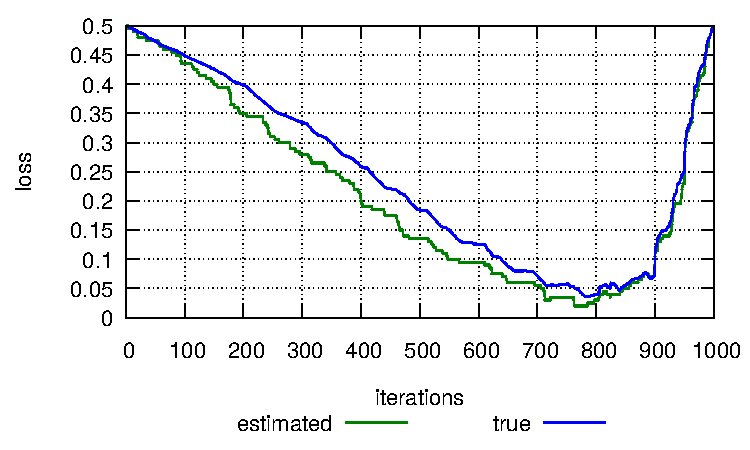
\includegraphics[trim=100 0 100 0, width=0.5\linewidth,valign=t]{figures/deDuplication/plot_simulated_s.pdf}
        \caption{Single linkage}
    \end{subfigure}%
    ~ 
    \begin{subfigure}[t]{0.5\textwidth}
        \centering
        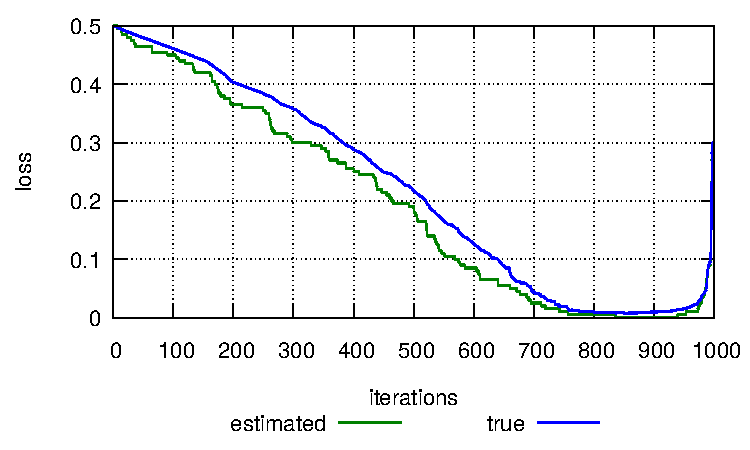
\includegraphics[trim=100 0 100 0, width=0.5\linewidth,valign=t]{figures/deDuplication/plot_simulated_c.pdf}
        \caption{Complete linkage}
    \end{subfigure}
	\caption{Simulated dataset: Loss reported for every iteration of hierarchical clustering}
    \label{fig:simulated}
\end{figure}

\begin{figure}[t]
    \centering
    \begin{subfigure}[t]{0.5\textwidth}
        \centering
        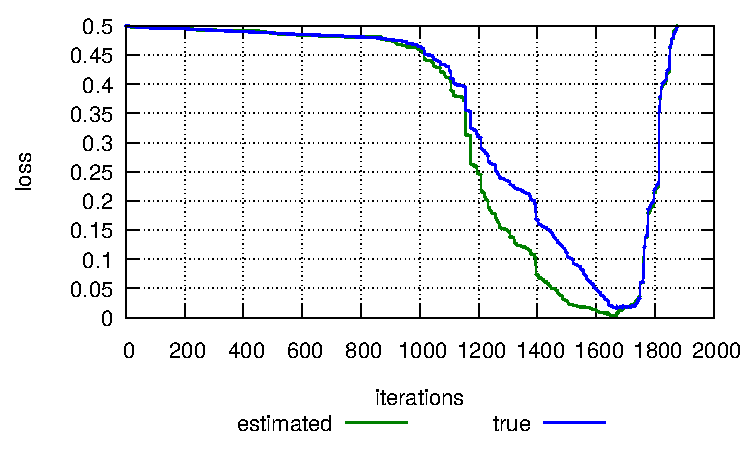
\includegraphics[trim=100 0 100 0, width=0.5\linewidth,valign=t]{figures/deDuplication/plot_real_s.pdf}
        \caption{Single linkage}
    \end{subfigure}%
    ~ 
    \begin{subfigure}[t]{0.5\textwidth}
        \centering
        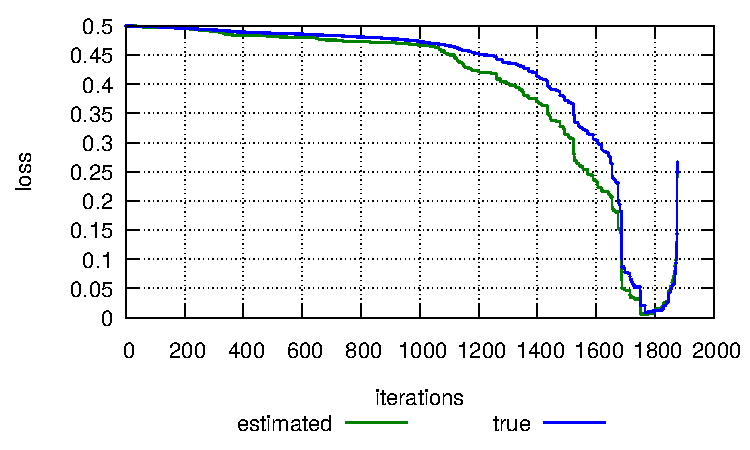
\includegraphics[trim=100 0 100 0, width=0.5\linewidth,valign=t]{figures/deDuplication/plot_real_c.pdf}
        \caption{Complete linkage}
    \end{subfigure}
	\caption{Publications dataset: Loss reported for every iteration of hierarchical clustering}
    \label{fig:publications}
\end{figure}

\begin{figure}[t]
    \centering
    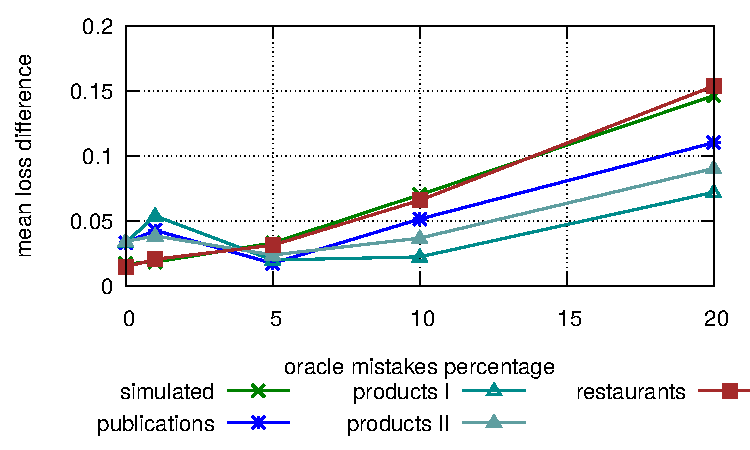
\includegraphics[trim=0 0 0 0, width=\linewidth,valign=t]{figures/deDuplication/plot_oracle_error.pdf}
    \caption{Impact of oracle mistakes}
    \label{fig:oracle-error}
\end{figure}
    



We now present the evaluation of our framework on a simulated and four real world datasets.
In Section \ref{sec:exp1} we show that our framework is generic and can be used to choose amongst many of the classes of algorithms for de-duplication. We also show that our framework can always choose a clustering which is close to the best clustering (algorithm) from a given class of clustering (algorithms) and our estimated loss for each of the clustering is very close to the true loss of these clustering algorithms.
In Section \ref{sec:exp2} we show that our framework is robust to upto 10\% of oracle mistakes, which far exceeds the intended settings dealing with human experts.
Finally, in Section \ref{sec:exp3} we show that in our framework a relatively small number of samples are enough to accurately estimate the loss of a clustering.

\subsection{Evaluation setup}
\label{sec:setup}
\textbf{Algorithms} In our evaluation we use four graph based clustering algorithms: (1) Articulation point clustering (\textit{ArtPt}) \cite{cormen2009introduction}, (2) Star clustering (\textit{Star}) \cite{aslam2006star}, (3) Approximate correlation clustering (\textit{ApproxCorr}) \cite{bansal2004correlation}, (4) Markov clustering (\textit{Markov}) \cite{van2000graph}. These graph based algorithms have been used for de-duplication problems as shown in previous work \cite{hassanzadeh2009framework}.
Hierarchical clustering algorithms are very effective and have been widely used to perform de-duplication. We consider 4 different linkage methods for hierarchical clustering: single linkage (C1), complete linkage (C2), weighted linkage (C3), and average linkage (C4). 
In addition to this we also implemented a heuristic based de-duplication algorithm (\textit{Na\"iveDedup}) where any two data points are considered similar if their distance is below a certain threshold. The output of this algorithm is pairs of data points which are marked similar.

\textbf{Datasets} For our evaluation we use five datasets.
First dataset is a simulated dataset of ten thousand strings of length 20 where we simulate a clustering over the set of strings and use it as our ground truth.
We use Jaro distance \cite{jaro1980unimatch} as the distance metric for strings.
To simulate a clustering we generate some seed strings and then for each seed string we generate multiple secondary strings by slightly editing the seed string.
Each cluster of strings resembles a single entity.
Second dataset is a real-world bibliographical information of scientific publications \cite{pubdata}.
The dataset has 1879 publication records with duplicates.
The ground truth of duplicates is available.
To perform clustering on this dataset we first tokenized each publication record and extracted 3-grams from them.
Then, on 3-grams we used Jaccard distance to define distance between two records.
Next two datasets are lists of E-commerce products: First dataset contains 1,363 products from Amazon, and 3,226 products from Google, and the ground truth has 1,300 matching products.
Second dataset contains 1,082 products from Abt, and 1,093 products from Buy, and the ground truth has 1,098 matching products. Both these products datasets are publicly available at \cite{products}. 
The fifth dataset is a list of 864 restaurants from the Fodor's and Zagat's restaurant guides that contains 112 duplicates. This dataset is also publicly available at \cite{restaurant}.
To perform clustering on the products and restaurants datasets we normalized the records (product or restaurant description) using standard techniques from natural language processing, namely; denoising text, word tokenization, normalization, and stemming and lemmatization. Given a record, this process gives us a list of word tokens. For each token, we first obtained a vector representation of the word using  \textit{Global Vectors} for word representations (GloVe \cite{jeffrey2014glove}). We averaged this representation across word tokens to obtain the representation of a single record. We use cosine similarity to define the distance between two records.
For the simulated and publications datasets, our distance metric was Jaccard and hence we use the MinHash \cite{broder2000min} as the hashing scheme. For the rest of the datasets, we used SimHash \cite{charikar2002similarity} as the hashing scheme. 
For all the datasets we use ground truth as the oracle that can answer \textit{same-cluster queries}. 
To calculate the true loss of a clustering (i.e. $L_{C^*}(C)$) we access all of the ground truth. Our framework uses only a sample of the ground truth to estimate the loss of a clustering.
To judge the performance of our framework we compare the estimated loss $\hat L_{C^*}(C)$ against the true loss.

\subsection{Clustering selection}
\label{sec:exp1}
In this experiment we demonstrate that our framework is generic and can be used to choose the best clustering algorithm amongst any of the classes of algorithms for de-duplication.
We used our framework on all the algorithms mentioned in Section \ref{sec:setup}. The results on five datasets are summarized in Table \ref{tab:exp3}. For each dataset we report the loss of the true-best clustering ($L_{C^*}(C)$) and the estimated loss of the best clustering selected by our framework $\hat L_{C^*}(C)$.
This experiment highlights two main features of our framework: (i) our framework can always choose a clustering close to the best clustering  algorithm from a given class of clustering algorithms using only a small number of samples, which is 200 (100 positive samples, and 100 negative samples) for all datasets and all the algorithms in Table \ref{tab:exp3}. (ii) Our estimated loss for each clustering is very close to the true loss of these clustering algorithms. At the bottom of the table we report the mean loss difference between estimated loss and true loss computed over all the algorithms. 

We would also like to emphasize that in our framework we sample only once for each dataset and use that  sample to estimate the loss of all the clusterings. In Figure \ref{fig:simulated} and \ref{fig:publications} we show that our sample can very closely estimate the loss of every clustering generated at each iteration of the hierarchical clustering. Similarly, for Table \ref{tab:exp3} we sampled only once for each dataset and evaluated all the clusterings generated by each algorithm.
Note that, each of the graph based algorithms have a hyper-parameter, i.e. the threshold on the edge weights. Edges with weights above this threshold represent dissimilar items and are pruned from the graph. For each of the graph based clustering algorithm we applied our framework on multiple values of the hyper-parameter and report only the ones with least true loss. However, for every choice of the hyper-parameter we observed that the estimated loss was very close to the true loss.

\subsection{Effect of oracle mistakes}
\label{sec:exp2}
In this experiment we show that our framework is effective in real-world scenarios where the oracle may not be perfect and can make mistakes. Whenever the oracle classifies a similar pair as dissimilar or a dissimilar pair as similar we count it as a mistake. In our datasets we artificially introduce such mistakes and vary their ratio from from 0\%, to 20\%. In Figure \ref{fig:oracle-error} we show that our framework can closely estimate the clustering loss up to 10\% of oracle mistakes, which, in real-world far exceeds the intended settings dealing with human experts. The Y-axis in Figure \ref{fig:oracle-error} reports the mean difference between true loss and estimated loss over all the clusterings selected in Table \ref{tab:exp3}.

%on four different methods of hierarchical clustering (C1 - C4). For each clustering, the goal is to find the pruning from the clustering tree that has minimum loss. We compare the loss of the best clustering found by our framework against the loss of the true-best clustering. We find the loss of the true-best clustering by performing all $|X|^2$ queries against the ground truth. In Table \ref{tab:exp3} we report the loss of the best clustering for all four clustering methods and both the datasets. In all the scenarios the best clustering picked by our framework is very close to the true-best clustering. The framework used 100 positive and 100 negative samples for this experiment for both the datasets. In Figures \ref{fig:simulated} and \ref{fig:publications}, we report the loss at every iteration of the hierarchical clustering. The loss reported by our framework is always close to the true loss of the clustering at every iteration. Another important point to note is that by only sampling 200 points, we are able to estimate the loss of all the clusterings (or prunings) of the hierarchical clustering tree.

\subsection{Impact of sample size}
\label{sec:exp3}

In this experiment we show that even a small number of samples are enough to estimate the true loss ($L_{C^*}(C)$).
%The true loss is computed by querying every pair $(x_1, x_2) \in X^{[2]}$ against the oracle (ground truth in our case).
We consider four different clusterings, each one picked at random from the four hierarchical clustering methods (C1 - C4).
Table \ref{tab:exp1} and \ref{tab:exp2} reports the loss for simulated and publications dataset, respectively.
For each dataset we increased the number of positive and negative samples and measured the loss.
The table also shows the true loss of the clustering.
It can be seen that the estimated loss calculated by our framework is close to the true loss even with 25 positive samples and 25 negative samples.
In addition to this, the loss does not change much by increasing the number of samples.
Which means that there is no incentive to sample more.
We also show that the number of queries performed by our framework are close to the sample size (as claimed in Thm. \ref{thm:queryComplexity}), which are orders of magnitude less than $O(|X|^2)$.
For example, in the simulated dataset and single linkage clustering (C1) with 25 positive and 25 negative samples our framework performed 51 queries, that means only one query was wasted. Similarly, 4 queries were wasted for 100 positive and 100 negative samples, and so on.

 
\ifdefined\COMPLETE
\else
\end{document}
\fi


\begin{subappendices}
\section{Locality Sensitive Hashing}
\label{section:A-LSH}
The technique of locality sensitive hashing was introduced by \cite{gionis1999similarity} to solve the problem of approximate nearest neighbour search. The LSH-based hashing schemes try to put similar points into the same bucket. Hence, to search for points which are `similar' to a given point $x \in X$, one only needs to search within the same hash bucket instead of searching within the whole set $X$. Next, we describe a generic hashing based algorithm. 

\begin{definition}[LSH \cite{charikar2002similarity}]
\label{defn:LSH}
Given a set $X$ and a similarity function $f:X \times X \rightarrow [0, 1]$. Given a class of hash functions $H = \{h_1, h_2, \ldots \}$. An LSH w.r.t $X$ and $f$ is a probability distribution over $H$ such that for each $x, y \in \mc X$, $$\underset{h \in H}{\mb P}\enspace [h(x) = h(y)] = f(x, y)$$
\end{definition}
\noindent Some common examples of an LSH schemes are minhash scheme w.r.t jaccard similarity measure \cite{broder2000min, broder1997resemblance}, simhash scheme w.r.t hamming similarity measure \cite{charikar2002similarity}. We describe a generic locality sensitive hashing procedure in Alg. \ref{alg:LSH}. Observe that, Alg. \ref{alg:LSH} outputs $s$ different partitions of $X$. Assume without loss of generality, that a point $x$ lies in the blocks $B_{11} \in P_1, B_{21} \in P_2, \ldots, B_{s1} \in P_s$. Now, to search for points $y$ which are similar to $x$, we only need to search within the blocks $B_{i1}$. We say that these points lie in the same `bucket' as $x$. We say that $b(x, y) = 1$ if and only if $x$ and $y$ lie together in the same block in atleast one of the partitions.

\begin{algorithm}
\caption{A generic LSH based hashing algorithm \cite{indyk1998approximate,charikar2002similarity}}
\label{alg:LSH}

\Indp\KwIn{A set $X$, a similarity function $f$, a class of hash functions $H$ over $X$, integers $r, s$ and a perfect hash function $p$ over the domain $\mb N^r$.}
\KwOut{Partitions $P_1, \ldots, P_s$ of the set $X$.}
\vspace{0.1in} Let $D$ be a distribution over $H$ which satisfies Defn. \ref{defn:LSH} and let $k = r s$.\\
Sample hash functions $h_1, \ldots, h_k$ iid using $D$.\\
 Group the hash functions into $s$ bands. Each band contains $r$ hash functions. \\
For all $x$ and $1\le i \le s$,  let $g_i(x) = (h_{(i-1)s + 1}(x), \ldots, h_{ir}(x))$. That is, $g_i(x)$ represents the $i^{th}$ signature of $x$. \\
For all $1 \le i \le s$, obtain partitions $P_i$ of $\mc X$. That is, $P_i = \{B_{i1}, \ldots, B_{im_i}\}$ where each $B_{ij} = \{x : p(g_i(x)) = b_{ij}\}$ for some $b_{ij}$.\\
Output $\{P_1, \ldots, P_s\}$.
\end{algorithm}



Hence, to search for points which are similar to $x$, we need to search over $y$ such that $b(x, y) = 1$. Our sampling procedure will sample pairs from the set $\mc Q := \{(x, y) : b(x, y) = 1\}$ (details in the next section). Hence, a requirement from the hashing scheme is that we should be able to construct the set $\mc Q$ in linear time. Thm. \ref{thm:hashTimeComplexity} shows that this is indeed the case. 

\begin{restatable}{thrm}{hashTimeComplexity}
\label{thm:hashTimeComplexity}
Given $X$, a similarity function $f$, a class of hash functions $H$, integers $r, s$ and perfect hash function $p$. Alg. \ref{alg:LSH} runs in $O(|X|rs \max_{ij}|B_{ij}|)$.
\end{restatable}
\begin{proof}
Let $n = |X|$. Sampling $k$ different hash function takes $rs$ time. Computing the signatures for all $x$ takes $nrs$ time. Obtaining the different partition takes $ns$ time. Now, computing $R_x$ for all $x$ takes time $t = \sum_{i = 1}^b \sum_{j=1}^{m_j} |B_{ij}|^2$. Now, we know that for all $i$, $\sum_{j=1}^{m_j} |B_{ij}| = n$. Hence, $\sum_{j=1}^{m_j} |B_{ij}|^2 \le \max_j B_{ij} \enspace \sum_{j=1}^{m_j} |B_{ij}| = n \max_j{B_{ij}}$. Hence, $t \le n s \max_{ij} |B_{ij}|$.  
\end{proof}

\noindent We see that the running time is dependent upon the block sizes. If the maximum block size is a constant then the hashing scheme runs in linear time. Even when the block sizes are bounded by $\log n$, then the scheme runs in $O(n \log n)$.  Next, we show that a if $d(x, y) \le \lambda$ then $(x, y) \in \mc Q$ with very high probability. Also, if $d(x, y) > O(2\lambda)$ then with high probability $(x, y) \not\in \mc Q$.   

\begin{restatable}{thrm}{similarInSame}
\label{thm:similarInSame}
Given a set $X$, a distance function $d: X \times X \rightarrow [0, 1]$, a class of hash functions $H$, threshold parameter $\lambda$ and a parameter $\delta$. Let the similarity function be $f(x, y) := 1 - d(x, y)$ and let $\mc A$ be a generic LSH based algorithm (Alg. \ref{alg:LSH}) which outputs partitions $P_1, \ldots, P_s$. Let $b(x, y) = 1$ iff $x, y$ are together in atleast one of these partitions. 
\noindent Choose $r, s$ such that $\frac{1}{2\lambda} < r < \frac{1}{-\ln(1-\lambda)} $ and $s =  \lceil 2.2\ln(\frac{1}{\delta})\rceil$. Define $\delta' := s\ln(1+\delta)$. Then for $(x, y) \in \mc X^2$
\begin{itemize}
	\item If $d(x, y) \le \lambda$ then 
	\begin{align*}
		& \underset{h \in H}{\mb P} \enspace[\enspace b(x, y) = 1 ] \enspace > \enspace 1 - \delta
	\end{align*}
	\item If $d(x, y) > 2\lambda\ln\big(1+\frac{1}{\delta}\big)$ then 
	\begin{align*}
		& \underset{h \in H}{\mb P} \enspace[\enspace b(x, y) = 1 ] \enspace < \enspace \delta'
	\end{align*}
\end{itemize}
\end{restatable}
\begin{proof}
Observe that
\begin{align*}
  & \mb P[b(x, y) = 0] = \mb P \enspace  [ \underset{i=1}{\cap^s} g_i(x) \neq g_i(y)] \\
  &=\prod_i\Big(1 - \prod_{j=1}^r \mb P[ h_{(i-1)r+j}(x) = h_{(i-1)r+j}(y)]\Big)\\
  & = \prod_{i=1}^s(1 - \prod_{j=1}^r f(x, y)) = (1-f(x, y)^r)^s
\end{align*}
Consider the case when $d(x, y) \le \lambda$. From the choice of $s$, we know that $s \ge 2.2\ln(1/\delta) \implies s \ge \frac{\ln(1/\delta)}{1-\ln(e-1)}\iff 1-\frac{1}{e} \le \delta^{1/s}$. From the choice of $r$, we know that $r < \frac{1}{-\ln(1-\lambda)} \iff r \ln(\frac{1}{1-\lambda}) < 1 \iff (1-\lambda)^r > \frac{1}{e}$.  Hence,   then we have that $\mb P[b(x, y) = 0]  = (1 - (1-d(x, y))^r)^s \le (1 - (1-\lambda)^r)^s < \delta$. This proves the first part of the theorem. 

For the second part, consider the case when $d(x, y) > \lambda'$ where $\lambda'$ is such that $\ln(1+1/\delta) = \frac{\lambda'}{2\lambda}$. 
\begin{flalign*}
  & \frac{1}{2\lambda} < r \iff \frac{\ln(1+1/\delta)}{\lambda'} < r. \enspace\text{Now, $\lambda' \le \ln\Big(\frac{1}{1-\lambda'}\Big)$. Hence, }&\\
  &\implies \frac{\ln(1+1/\delta)}{\ln(\frac{1}{1-\lambda'})} < r \iff r\ln(1-\lambda') < \ln(\frac{\delta}{1+\delta}) &\\
  &\iff 1-(1-\lambda')^r > e^{-\ln(1+\delta)} = e^{-\delta'/s} > (1-\delta')^{1/s}&\\
  &\implies \mb P[b(x, y) = 0] > (1-(1-\lambda')^r)^s > 1-\delta'&
\end{flalign*}
Now, the only thing that remains to be shown is that we can choose an integer $r$ satisfying the conditions of the theorem. Consider the function $f(x) = -\frac{1}{2x} - \frac{1}{\ln(1-x)}$. Using elementary analysis, we see that for $x \rightarrow 0, f(x) \rightarrow \infty$. Infact, for $x \le 0.32, f(x) > 1$. Hence, for $\lambda \le 0.32$, $r$ satisfying the conditions of the theorem exists.
\end{proof}

\section{Sample and query complexity of RCC using $\mc P_{12}$}
\begin{restatable}{thrm}{sampleComplexityLSH}
Given metric space $(X, d)$, a class of clusterings $\mc F$ of $X$ and a threshold parameter $\lambda$. Given $\epsilon, \delta \in (0, 1)$ and a $C^*$-oracle. Let $d$ be $(\alpha, \beta)$-informative w.r.t $C^*$ and $\lambda$ and let $X$ satisfy $\gamma$-skewed property. Let $\mc A$ be the ERM-based approach as described in Alg. \ref{alg:ERM} (where the LSH-based scheme is $\zeta$-tight) and $\hat C$ be the output of $\mc A$. If  
\label{thm:sampleComplexityLSH}
\begin{align}
  &m_-, m_+ \enspace \ge a\frac{\vcdim({\mc F}) + \log(\frac{2}{\delta})}{\epsilon^2} 
\end{align}
where $a$ is a global constant then with probability atleast $1-\delta - \exp\big(\frac{-2\nu^2(1-\alpha)^2|X_2^+|^2}{49}\big)$ (over the randomness in $\mc A$), we have that $$L_{C^*}(\hat C) \enspace\le\enspace \min_{\mc C \in \mc F} L_{C^*}(C) + 3\alpha + \zeta + \epsilon + \nu$$
\end{restatable}
\begin{proof}
Let $T_0$ be the distribution induced by $\mc P_0$ and $T_1$ be the distribution induced by $\mc P_1$. Using Thm. \ref{thm:uniformConvergence}, we know that if $m_+ > a\frac{\vcdim({\mc F}) + \log(\frac{1}{\delta})}{\epsilon^2}$ then with probability atleast $1-\delta - e^{-2\nu^2(1-\alpha)^2|X_2^+|^2}$, we have that for all $C$
\begin{align*}
  &|\hat P(C) - \underset{(x,y) \sim T_1}{\mb P}[C(x, y) = 0]| \le \epsilon\\
  \implies &\hat P(C) \le \epsilon + (1+2\nu)(1+2\alpha)L_{P^+}(C) \enspace\text{ and}\\
  &L_{P^+}(C) - \epsilon - \alpha -\zeta - \nu \le \hat P(C) \numberthis \label{eqn:eHatLSH}
\end{align*}
Note that we obtain upper and lower bounds for $\underset{(x,y) \sim T_1}{\mb P}[h(x, y) = 0]$ using Thm. \ref{thm:posDistributionLSH}. Similarly, if $m_- > a\frac{\vcdim({\mc F}) + \log(\frac{1}{\delta})}{\epsilon^2}$, then with probability atleast $1-\delta$, we have that for all $h$,
\begin{align*}
  &|\hat N(C) - \underset{(x,y) \sim T_0}{\mb P}[C(x, y) = 1]| \le \epsilon\\
  \implies &\hat N(C) \le \epsilon + L_{P^-}(C) \enspace\text{ and } L_{P^-}(C) -\epsilon \le \hat N(C) \numberthis\label{eqn:gHatLSH}
\end{align*}

\noindent Combining Eqns. \ref{eqn:eHatLSH} and \ref{eqn:gHatLSH}, we get that with probability atleast $1-2\delta-e^{-2\nu^2(1-\alpha)^2|X_2^+|^2}$, we have that for all $C \in {\mc F}$
\begin{align*}
  \hat L(C) &\le \mu [\epsilon + (1+2\nu)(1+2\alpha)L_{P^+}(C)]\\
  &+ (1-\mu)(\epsilon + L_{P^-}(C))\\
  &\le L_{C^*}(C) + \epsilon + 2\alpha + 2\nu + 4\alpha\nu\\
  \text{And} \enspace \hat L(C) &\ge \mu(L_{P^+}(h) -\epsilon - \alpha - \nu-\zeta) + (1-\mu)(L_{P^-}(h) - \epsilon) \\
  &\ge L_{C^*}(C) - \epsilon - \alpha - \nu - \zeta
\end{align*}
Now, let $\hat C$ be the output of $\mc A$ and let $\hat C^*$ be $\argmin_{C \in {\mc F}} L_{C^*}(C)$. Then, we have that
\begin{align*}
  L_{C^*}(\hat C) &\le \hat L(\hat C) + \alpha + \epsilon + \nu +\zeta \le \hat L(\hat C^*) + \alpha + \epsilon + \nu +\zeta\\
  &\le L_{C^*}(\hat C^*) + 2\epsilon + 3\alpha + 3\nu + 4\alpha\nu + \zeta
\end{align*}

Choosing $\epsilon = \frac{\epsilon}{2}$ and $\delta = \frac{\delta}{2}$ and $\nu = \frac{\nu}{7}$ throughout gives the result of the theorem,
and this completes the proof of the theorem.
\end{proof}

Finally, we analyse the query complexity of our approach. That is the number of queries that our algorithm makes to the $C^*$-oracle. Our algorithm makes queries during the sampling procedure. We see that to sample $m_-$ negative and $m_+$ positive pairs the number of queries is `close' to $m_+ + m_-$ with very high probability. Thus, the number of `wasted' queries is small.  

\begin{restatable}{thrm}{queryComplexityLSH}[Query Complexity]
\label{thm:queryComplexity}
Let the framework be as in Thm. \ref{thm:sampleComplexityLSH}. With probability atleast $1-\exp\big(-\frac{\nu^2m_-}{4}) - \exp\big(-\frac{\nu^2m_+}{4}\big) - \exp(-\nu^2(1-\alpha)^2|\mc X_+^2|^2)$ over the randomness in the sampling procedure, the number of same-cluster queries $q$ made by $\mc A$ is  
$$q \le (1+\nu)\bigg(\frac{m_-}{(1-\gamma)} + \frac{m_+}{\beta(1-\zeta-\nu)}\bigg)$$
\end{restatable}

\begin{proof}
The number of queries made to sample the set $S_g$ is $q_g = m_g$. Let $q_+$ denote the number queries to sample the set $S_+$. Using Lemma \ref{lemma:posQueriesLSH}, we know that $\mb E[q_+] \le \frac{1}{\beta(1-\zeta-\nu)}$ with probability atleast $1-\exp(-\nu^2(1-\alpha)^2|\mc X_+^2|^2)$ over the randomness in the hashing procedure. Given that the expectation is bounded as above, using Thm. \ref{thm:geometricRV}, we get that $q_+ \le \frac{(1+\nu)m_+}{\beta(1-\zeta-\nu)}$ with probability atleast $1-\exp(\frac{-\nu^2m_+}{4})$. Similarly, combining Lemma \ref{lemma:negQueries} with Thm. \ref{thm:geometricRV}, we get that with probability atleast $1-\exp(\frac{-\nu^2m_-}{4})$, $q_- \le \frac{(1+\nu)m_-}{(1-\gamma)}$.
\end{proof}
\end{subappendices}

\chapter{Noise-robust clustering}
\label{chapter:optimizationClustering}
\ifdefined\COMPLETE
\else
\documentclass[12pt]{article}

\usepackage{algorithm}
\usepackage{mathtools,amsmath,amssymb,amstext,amsthm,tikz,thmtools}
\usepackage[inline]{enumitem}

\usepackage[utf8]{inputenc} % allow utf-8 input
\usepackage[T1]{fontenc}    % use 8-bit T1 fonts
\usepackage{hyperref}       % hyperlinks
\usepackage{url}            % simple URL typesetting
\usepackage{booktabs}       % professional-quality tables
\usepackage{amsfonts}       % blackboard math symbols
\usepackage{nicefrac}       % compact symbols for 1/2, etc.
\usepackage{microtype}      % microtypography

\newcommand{\mc}{\mathcal}
\newcommand{\mb}{\mathbf}
\newcommand{\tr}{\text{Tr}}
\newcommand{\diag}{\text{diag}}
\newcommand\numberthis{\addtocounter{equation}{1}\tag{\theequation}}

\DeclareMathOperator*{\argmin}{arg\,min}
\DeclareMathOperator*{\argmax}{arg\,max}

\newtheorem{theorem}{Theorem}
\newtheorem{lemma}[theorem]{Lemma}
\newtheorem{definition}[theorem]{Definition}
\newtheorem{proposition}[theorem]{Proposition}
\newtheorem{corollary}[theorem]{Corollary}

\begin{document}
\fi

Clustering aims to group similar data instances together while separating dissimilar ones. However, often many datasets have, on top of cohesive groups, a subset of ``unstructured'' points as well. In such cases, the goal is to detect the structure while simultaneously separating the unstructured data points. Clustering algorithms that achieve this goal are said to be {\em robust} to noise.

The most common approach to clustering views it as an optimization problem. The idea is to associate a cost (or objective) with each possible partition of the input dataset (into $k$ subsets) and then try to find a partition which has minimum cost. Examples of common objective functions include $k$-means and $k$-median cost functions. However, these common objective functions are not robust to the presence of noise.   

In this chapter, we propose a generic method of regularization that can transforms any clustering objective which outputs $k$ clusters to one that outputs $k+1$ clusters. The algorithm is now allowed to `discard' points into an extra `garbage' or noise cluster by paying a constant regularization penalty. The intuition is that allowing the clustering algorithm to discard a few points should make it easier to detect the structure in the remaining non-noisy points. However, we prove that finding the optimal solution to the regularized objective is NP-Hard \footnote{Throughout this chapter, we consider the standard and regularized versions of the $k$-means objective}. The goal is to develop an efficient clustering algorithm which is provably noise-robust.
%Similar to regularisation, {\em noise prototypes} (points which are equidistant to all other points) were considered by \cite{dave1993robust}. However, that idea was used only in the limited context of Lloyd’s algorithm and without any theoretical or noise robustness guarantees.

From a theoretical perspective, one common approach to dealing with such hardness results is the following. (i) Consider a convex relaxation of the original objective function (which can be efficiently solved using standard techniques). (ii) Prove that under certain data niceness conditions the solution obtained by solving the relaxed objective function coincides with the optimal solution of the original objective function. For example, \cite{peng2007approximating} used this strategy to design an algorithm based on the sdp-relaxation of the $k$-means objective function. \cite{awasthi2015relax} proved that under the `stochastic ball assumption', the solution of the sdp-based approach is indeed the optimal $k$-means clustering. 

One advantage of studying convex relaxations of clustering objectives over other clustering heuristics (like the llyod's algorithm \cite{lloyd1982least}) is that we can verify when the output solution is optimal. There was been lot of work in analyzing clustering algorithms under distributional and clusterability assumptions (see \cite{balcan2012clustering}, \cite{awasthi2012center}, \cite{kalai2010efficiently}, , \cite{achlioptas2005spectral, \cite{sanjeev2001learning}} and \cite{hsu2013learning} and the references therein). However, often the algorithms are designed keeping the input conditions in mind. Convex relaxations have an advantage that they are not specifically tailored to a particular distribution. In this chapter, we use this approach (sdp relaxation of the regularized $k$-means objective) to design an efficient and noise-robust clustering algorithm.

Our framework is the following. We are given an input dataset $X$ made of two components. The first is the clusterable subset $I$ which satisfies a niceness property. Namely, $I$ is the union of $k$ unit balls $B_i$ each separated by a distance of atleast $\delta$. The second is the unstructured or noise component $N$. Note that the clustering algorithm only sees $X$ and is not aware of $I$ or $N$. The goal is to design an efficient clustering algorithm $\mc A$ such that the output of the algorithm $\mc A(X)$ when restricted to $I$, is able to detect and recover the structure of $I$ (namely, the balls $B_i$). In this chapter, we consider two choices for $\mc A$. The first based on SDP relaxation of the regularized $k$-means objective and the second based on the LP relaxation. For the noiseless case, \cite{awasthi2015relax} showed that for $\delta > 2\sqrt{2}(1+1/\sqrt d)$ (where $d$ is the dimension of the euclidean space) the algorithm based on SDP-relaxation of the standard $k$-means objective recovers (with high probability) the structure of $I$ if the balls $B_i$ are generated by an isotropic distribution (stochastic ball model \cite{iguchi2015tightness}, \cite{iguchi2017probably}, \cite{awasthi2015relax} and \cite{nellore2015recovery}).

In this chapter, we improve over previous results and give success guarantees in the regime $\delta > 2(1+\sqrt{k/d})$ which is near-optimal for large $d$. In the presence of noise, we prove that the algorithm based on the SDP-relaxation of the regularized objective recovers the clustering of $I$ for $\delta > 2(1+\sqrt{\zeta + k/d})$. Here $\zeta$ is a term which depends on the ratio of number of noisy points and the number of points in the smallest cluster. We obtain similar results for the LP based algorithm as well. However, in that the case both separation requirement and the restrictions on noise are stronger.  

We also conduct simulation studies where we examine the effect of $\lambda$, the number of noisy points $m$, the separation $\delta$ and other parameters on the performance of our regularised SDP-based algorithm. We also perform experiments on the MNIST dataset. We observed that the regularised version performed better than $k$-means++ when the dataset had noisy points. In the absence of noise, the performance of both these algorithms were similar. 

\section{Related Work}
\begin{table}
\centering
\caption{Known results for clustering under stochastic ball model. The columns show the separation under which recovery guarantees hold. All these results are for the noise-less case}

\label{table:stochasticBall}
\setlength{\tabcolsep}{0.5em} 
{\renewcommand{\arraystretch}{1.2}%
\begin{tabular}{llc}
\\
 & Separation condition & Reference\\
 \hline
$k$-median LP & $\delta > 3.75$ & Thm. 1 in \cite{nellore2015recovery}\\
 & $\delta > 2$ & Thm. 1 in \cite{awasthi2015relax}\\
\hline
$k$-means LP & $\delta > 4$ & Thm. 9 in \cite{nellore2015recovery}\\
\hline
$k$-means SDP & $\delta > 2\sqrt2 (1 + \frac{1}{\sqrt d})$ & Thm. 3 in \cite{awasthi2015relax}\\
 & $\delta > 2 + \frac{k^2}{d}cond(\gamma)$ & Thm. 2 in \cite{iguchi2015tightness}\\
 & $\delta > 2 + \frac{k^2}{d}$ & Thm. 9 in \cite{iguchi2017probably}\\
 & $\delta > 2 + \sqrt{\frac{k}{d}}$ & Thm. \ref {thm:SDPGeneral}\\
\hline


\label{table:alphacenter}
\end{tabular}
}
\end{table}
The problem of robustifying a clustering objective function has been studied before. \cite{ben2014clustering} give a generic procedure that can transform any clustering objective with metric $d$ to an objective function which uses $d'$ which is a truncated version of the original metric. More specifically, $d'(x, y) = \min (\lambda,   d(x,y)).$ Then they show that if there exists an algorithm which can solve the optimization problem then such an algorithm is robust to noise. \cite{georgogiannis2016robust}  also studies breakdown properties of the truncated objective function, that is the number of outliers which can cause significant change in the estimates of any one of the centers. However, it is unclear as to how we would solve the optimization problem. In this work, we propose an efficient algorithm based on convex relaxation of our regularized objective function and give robustness guarantees for the same. 

The problem of recovering the underlying cluster structure in the presence and absence of noise has been studied before both in distribution-free and distribution-based settings. In the distribution-free setting, the goal is to prove that if the data has some structure (is {\em clusterable}) then the (proposed or existing) clustering algorithm recovers that structure in the presence or absence of noise. Such works, make no assumption on the distribution that generated the data. Different works define different notions of `clusterable' data. In the current work, the separation requirement on the clusters was global. That is, the each cluster was separated by atleast $\delta$ times the maximum radius amongst all the clusters. Another popular notion of clusterability is $\alpha$-center proximity \cite{awasthi2012center} which requires that two clusters be separated relative to their radii. \cite{balcan2012clustering} consider a dataset which has $\alpha$-center proximity except for an $\epsilon$-fraction of points. They propose an efficient algorithm which provides an $1+O(\epsilon)$ approximation to the optimal $k$-median solution for $\alpha > 2 + \sqrt{7}$.

In this work, we assume that the input satisfies the stochastic ball assumption. This model was considered by \cite{nellore2015recovery} in the context of LP relaxation of the $k$-median objective function. They showed that if the separation between the clusters $\delta > 3.75$, then the lp relaxation finds the desired clustering. This bound was later improved to $\delta > 2$ in \cite{awasthi2015relax}. They also considered the LP relaxation of $k$-means objective and gave recovery guarantees when $\delta > 4$. They also considered the sdp relaxation of the $k$-means objective. They showed similar recovery guarantees when $\delta > 2\sqrt 2 (1 + \sqrt d)$. This bound was later improved to $\delta > 2 + k^2/d$ by \cite{iguchi2017probably}. Table \ref{table:stochasticBall} contains a summary of the various results under the stochastic ball model. These results however apply only to the noiseless case. In this chapter, we consider the same framework but prove recovery guarantees even in the presence of a small fraction of noisy points. 

Another line of work, which has some similarities to the framework in this chapter is estimating the parameters of a distribution in the presence of noise. \cite{lai2016agnostic} considered the problem of mean estimation of a gaussian when $\epsilon$ fraction of the points are corrupted by noise and propose an efficient algorithm that can estimate it with almost linear samples. \cite{diakonikolas2016robust} acheive an error of $O(\epsilon\sqrt{\log \epsilon})$ for mean estimation which was later improved to $O(\sqrt\epsilon)$ \cite{diakonikolas2017being}, \cite{steinhardt2018resilience}. \cite{charikar2017learning} and \cite{diakonikolas2016robust} considered the problem of recovering a mixture of $k$ gaussians with few adversaries. \cite{charikar2017learning} show that it is possible to recover the means when the separation between the means is $\tilde \Omega(\sigma \sqrt{k})$ where $\sigma^2$ is an upper bound on the variance of the $k$ gaussians. \cite{diakonikolas2016robust} output a distribution which is close to the target distribution in total variation distance. However, their run-time is exponential in $k$. In this chapter our focus is on understanding the robustness properties of convex-relaxation type algorithms (specifically those based on relaxation of our regularized objective). Hence, these results our orthogonal to the current discussion.  

%Different works on clustering have also made different assumptions on the type of noisy points. The most common is to assume that the noise is adversarial but the number of adversaries is not too large. For example,  and  provide bounds for clustering in the presence of noise as long as the number of adversaries is constant-factor smaller compared to the size of the smallest cluster. \cite{kushagra2016finding} considered noise which is structureless, that is the noisy points do not form dense large subsets. Another field of work is to address noisy part of the data as being generated by some uniform random noise or gaussian perturbations \cite{cuesta1997trimmed}, \cite{garcia2008general} and \cite{dave1993robust}. Some works examine the robustness of different algorithms when the number of clusters is the same for the original data and the data with added noise. They show that in this setting the traditional algorithms are provably not noise-robust \cite{hennig2008dissolution} and \cite{ackerman2013clustering}. 

\cite{peng2007approximating} formulated the $k$-means objective as a 0-1 SDP and proved equivalence between the two formulations. They then relaxed the 0-1 SDP to a standard SDP. In this work, we use a similar proof and relaxation technique but for the regularised $k$-means objective. 

\section{Preliminaries and definition}
\label{sec:pre}

Let $(\mb M, d)$ be a metric space. Given a finite set $\mc X \subset \mb M$, a $k$-clustering $\mc C$ of $\mc X$ partitions the set into $k$ disjoint subsets $\mc C = \{C_1, \ldots, C_k\}$. An objective-based clustering algorithm associates a cost with each possible partition of $\mc X$ and then tries to find the clustering with minimum cost. Throughout this section, $f$ denotes a function on the nonnegative reals.

\begin{definition}[$(k, f)$-objective algorithm] Given $\mc X\subset \mb M$ and a distance function $d$, a $(k, f)$-objective based algorithm $\mc A$ tries to find centers $\mu_1, \ldots, \mu_k \in \mb M$ so as to minimize the following function
\begin{align}
\label{eqn:kfObjectiveAlg}
\text{Cost}(\mu_1, \ldots, \mu_k) = \sum_{x\in \mc X} f(d(x, \mu(x))), \quad \mu(x) = \argmin_{\mu \in \{\mu_1, \ldots, \mu_k\}} d(x, \mu).
\end{align}
\end{definition}
Note that algorithm $\mc A$ may not often find the optimal solution because for many common functions $f$, solving the optimization is NP-Hard. Thus, heuristics are used that can get stuck at a local minima. For example, when $f(x) = x^2$, the above definition corresponds to the $k$-means objective, and the Lloyd's algorithm that is used to solve this objective can get stuck at a local minima. 

\begin{definition}[$(k, f)$-$\lambda$-regularised objective algorithm] Given $\mc X\subset \mb M$ and a distance function $d$, a $(k, f)$-$\lambda$-regularised objective based algorithm $\mc A'$ tries to find centers $\mu_1, \ldots, \mu_k \in \mb M$ and set $\mc I\subseteq \mc X$ so as to minimize the following function
\begin{align}
\label{eqn:kfObjectiveAlg}
\text{Cost}(\mu_1, \ldots, \mu_k, \mc I) = \sum_{x\in \mc I} f(d(x, \mu(x))) + \lambda |\mc X \setminus \mc I|,
\end{align}
where $\mu(x) = \argmin_{\mu_i} d(x, \mu_i).$
\end{definition}

The regularised objective allows discarding certain points into a ``garbage'' cluster at the expense of paying a constant penalty. The intuition is that this will help the algorithm better detect the structure of the remaining points. We will see in \S \ref{section:hardness} that minimizing this objective function is NP-Hard for all $k \ge 1$.

\subsection{Robustification paradigms}
\begin{definition}[$\lambda$-Regularised Paradigm] The $\lambda$-regularised paradigm is a robustification paradigm which takes as input a $(k, f)$-objective algorithm $\mc A$ and returns a $(k, f)$-$\lambda$-regularised objective algorithm $\mc A'$.  
\end{definition}

In this work, we focus on robustification of the $k$-means objective. Hence, it is useful to define the regularised $k$-means objective as we will refer to it many times in the remainder of the chapter. 

\subsection{Regularised $k$-means objective}
Given a finite set $\mc X \subset \mb R^{d}$ and an integer $k$, the regularised $k$-means objective aims to partition the data into $k+1$ clusters $\mc C = \{C_1, \ldots, C_{k}, C_{k+1}\}$ so as to solve 
% Changed to put min in objective; seems clearer to me -Nicole
\begin{align}
	\min_{C_1,\ldots, C_{k+1} \atop c_1, \ldots, c_k} \sum_{i=1}^k \sum_{x \in C_i} \|x-c_i\|_2^2 + \lambda |C_{k+1}|.
	\label{eqn:modifiedkmeans}
\end{align}

Note that the first term of the objective depends on the $l_2$ norm, while the second term depends only on the cardinality of the ``noise'' cluster. In order to make our objective function invariant to scaling, the regularization constant $\lambda$ is added to the cost function. 

Let $m(\mc X) := \min_{x\ne y \in \mc X} \|x-y\|_2^2$ and $N = |\mc X|$. Then, it is easy to see when $\lambda \leq \frac{m(\mc X)}{2}$, then \eqref{eqn:modifiedkmeans} admits a trivial solution: each cluster $C_i$ for $i \leq k$ has exactly one point and all the remaining points are in $C_{k+1}$, leading to an objective $\lambda (N-k)$. Indeed, for any other clustering with $|C_i| = n_i$ its objective is at least $\sum_{i=1}^k (n_i-1) m(\mc X)/2 + \lambda n_{k+1} = (n-n_{k+1} - k) m(\mc X)/2 + \lambda n_{k+1}$, where we have used the simple fact:
\begin{align}
\forall C \subset \mc X, ~~
\min_{c} \sum_{x \in C} \|x - c\|_2^2 ~=~ \frac{1}{2|C|}\sum_{x, y \in C} \|x - y\|_2^2.
\end{align}
Comparing the objectives we see the solution is indeed trivial when $\lambda \leq m(\mc X) /2$. Surprisingly, for the interesting case when $\lambda > m(\mc X) /2$, the problem suddenly becomes NP-Hard, as we prove below.

\subsection{Robustness measure}
Given two clusterings $\mc C$ and $\mc C'$ of the same set $\mc X$, we define the distance between them, $\Delta(\mc C, \mc C')$, as the fraction of pairs of points which are clustered differently in $\mc C$ than in $\mc C'$. % I changed this sentence because it didn't make sense -- is this equivalent to what you meant?. -Nicole
Given $\mc I \subseteq \mc X$, $\mc C|\mc I$ denotes the restriction of the clustering $\mc C$ to the set $\mc I$.

\begin{definition}[$\gamma$-robust \cite{ben2014clustering}]
Given $\mc X\subset \mb M$ and clustering algorithm $\mc A$, let $\mc A'$ be its robustified version obtained using any robustification paradigm. Given $\mc I \subseteq \mc X$, we say that $\mc I$ is $\gamma$-robust w.r.t $\mc X \setminus \mc I$ and $\mc A'$ if 
\begin{align}
\Delta(\mc A'(\mc X)|\mc I, \mc A(\mc I)) \le \gamma
\end{align}
\end{definition}
This measure tries to quantify the difference in the clustering of the set $\mc I$ after the addition of `noisy' points $\mc X \setminus \mc I$. If $\mc A'$ is indeed robust to noisy points, then the clusterings should be similar. 



\section{Hardness of regularised $k$-means}
\label{section:hardness}

In this section, we present hardness results for the regularised $k$-means objective. 
%Before we discuss the hardness results, it is worthwhile to mention the trivial case when $\lambda = 0$. In this case the optimization problem is easy and corresponds to the trivial solution of putting every point in the noise cluster $C_{k+1}$. 
The proof for $k \ge 2$ is fairly straightforward and follows from known hardness results for the standard (non-regularised) $k$-means. The more interesting case is when $k = 1$. It is well-known that $1$-means can be solved in linear time \cite{Bellman73} hence the same reduction does not work any more. We reduce an instance of the MAX-CLIQUE problem to the regularised $1$-means problem. We give a proof sketch for the reader's intuition. The technical details can be found in the supplementary section.

%\begin{restatable}{theorem}{hardForAvgdist}\label{lemma:hardForAvgdist}
%Given a clustering instance $\mc X \subset \mb R^d$ and $k \ge 2$, finding the optimal solution to the regularised $k$-means objective is NP-Hard for $\lambda > 0 $.
%\end{restatable}
%\begin{proof}[Proof sketch]
%The idea is as follows. We first show that for a ``big enough'' $\lambda$, the problem is NP-Hard. This is because for a sufficiently large value of $\lambda$, any optimal solution of regularised $k$-means will set $C_{k+1} = \emptyset$, in which case regularised $k$-means reduces to $k$-means, which is known to be NP-Hard \cite{dasgupta2008hardness}. Next, using a scaling argument we show that if the problem is NP-Hard for one $\lambda$, then it is NP-Hard for all $\lambda > 0$.  
%\end{proof}

\begin{restatable}{theorem}{hardForkone}
\label{theorem:hardFork1}
Given a clustering instance $\mc X \subset \mb R^d$. Finding the optimal solution to the regularised $1$-means objective is NP-Hard for all $\lambda > m(\mc X)/2$, where recall that $m(\mc X) := \min_{x\ne y \in \mc X} \|x-y\|_2^2$.
\end{restatable}

\begin{proof}[Proof sketch]
The proof has two parts. We first show that for fixed $\lambda$ the problem is NP-Hard. The proof works by reducing an instance of MAX-CLIQUE to the regularised $1$-mean instance. The idea is to define the distance between any pair of vertices as $1$ if there exists an edge between them. If not, then define the distance as $1 + \Delta$ for a suitably chosen $\Delta$. This construction guarentees that the problem is NP-Hard for atleast one $\lambda > \frac{m(\mc X)}{2}$. Next, using a scaling argument we show that if the problem is NP-Hard for one particular $\lambda$, then it is NP-Hard for all $\lambda > \frac{m(\mc X)}{2}$.
\end{proof}

The above theorem infact shows that regularised $k$-means is hard for all $k \ge 1$. This is becuase we can reduce an instance of regularised $1$-means to regularised $k$-means by placing $k-1$ points very far away. 

\section{The regularised $k$-means SDP-based algorithm}
\label{section:heuristic}
In the previous section, we showed that the regularised $k$-means objective is NP-Hard to optimize. Hence, we cannot hope to solve the problem exactly unless $P=NP$. In this section, we develop an algorithm based on semi-definite programming relaxation of the regularised objective. 

\cite{peng2007approximating} developed an algorithm $\mc A$ (Alg. \ref{alg:heuristicSDP} with $\lambda = \infty$) which tries to minimize the $k$-means objective. They obtained a convex relaxation of the $k$-means objective and solved it polynomially using standard solvers. In this section, we use the same technique to obtain and efficiently solve the convex relaxation of the regularised $k$-means objective. Our algorithm $\mc A'$ (Alg. \ref{alg:heuristicSDP}) is the robustified version of $\mc A$ using the $\lambda$-regularised paradigm. In \S \ref{subsection:sdpAlg}, we give the details of how we transform the regularised objective into an SDP. \S \ref{subsection:sdpRobust} has our main results where we give robustness guarentees for $\mc A'$.    

\begin{algorithm}[t]
\caption{SDP-based regularised $k$-means algorithm}
\label{alg:heuristicSDP}
	\textbf{Input: }{ $\mc{X} \subset R^d$, $k$, and hyperparameter $\lambda$.} \\
	\textbf{Output: }{$\mc C' := \{C_1, \ldots, C_k, C_{k+1}$\}.}
	
	Compute the matrix $D_{ij} = \|x_i-x_j\|^2_2$.\\
	Solve the SDP (Eqn. \ref{eqn:regularisedSDP}) using any standard SDP solver and obtain matrix $Z$ and vector $y$.\\
	Use the rounding procedure (Alg. \ref{alg:roundSDP}) to obtain the partition $\mc C'$. 
\end{algorithm}

 
\subsection{The SDP-based algorithm}
\label{subsection:sdpAlg}
The SDP relaxation of the regularised $k$-means objective is obtained in two steps. Using similar technique to that of \cite{peng2007approximating}, we translate Eqn. \ref{eqn:modifiedkmeans} into a 0-1 SDP (Eqn. \ref{eqn:regularisedSDP}). We then prove that solving the 0-1 SDP exactly is equivalent to solving the regularised $k$-means problem exactly. Then, we relax some of the constraints of the 0-1 SDP to obtain a tractable SDP which we then solve using standard solvers. We then describe the rounding procedure which uses the solution of the SDP to construct a clustering of the original dataset. 

\begin{equation*}
	\begin{split}
	\textbf{0-1}\\
	\textbf{SDP}
  \end{split}
	\begin{cases}
		\min_{Z, y} \enspace &\tr(DZ) + \lambda \langle \mb 1, y\rangle\\
		\text{s.t. } \enspace &\tr(Z) = k\\
		& Z\cdot \mb 1 + y = \mb 1\\	
		&Z\ge 0, Z^2 = Z, Z^T = Z \\
		& y \in \{0, 1\}^n
	\end{cases}
	\xrightarrow{\text{relaxed}} \textbf{ SDP } 
	\begin{cases}
		\min_{Z, y} \enspace &\tr(DZ) + \lambda \langle \mb 1, y\rangle\\
        \text{s.t. } \enspace &\tr(Z) = k\\
		& \Big(\frac{Z+Z^T}{2}\Big)\cdot \mb 1 + y = \mb 1\\		
		&Z \ge 0, y \ge 0, Z \succeq 0 \numberthis\label{eqn:regularisedSDP}
	\end{cases}
\end{equation*}

\begin{restatable}{theorem}{modifiedkmeans}
\label{thm:modifiedkmeans}
Finding a solution to the 0-1 SDP (\ref{eqn:regularisedSDP}) is equivalent to finding a solution to the regularised $k$-means objective (\ref{eqn:modifiedkmeans}). 
\end{restatable}

Equation \ref{eqn:regularisedSDP} shows our 0-1 SDP formulation. The optimization is NP-Hard as it is equivalent to the regularised $k$-means objective. Hence, we consider a convex relaxation of the same. First, we replace $Z^2 = Z$ with $Z \succeq 0$. In addition, we relax $y \in \{0, 1\}^n$ to $y \geq 0$, as the constraint $y\leq 1$ is redundant. Using these relaxations, we obtain the SDP formulation for our objective function.

We solve the SDP using standard solvers \cite{yang2015sdpnal+} thereby obtaining $Z, y$. 
The proof of Thm. \ref{thm:modifiedkmeans} showed that the optimal solution of 0-1 SDP is of the following form. $Z$ is a $n\times n$ block diagonal matrix of the form $\diag(Z_{I_1}, \ldots, Z_{I_k}, 0)$, where $n = |\mc X|$ and $Z_{I_i} = \frac{1}{|C_i|}11^T$. Thus, given $Z$, we can extract the set of cluster centers $C = ZX$ which is an $n \times d$ matrix. Each row $C_i$ contains the cluster center to which data point $x_i$ belongs. For the points $x_j$ assigned to the noise cluster, the corresponding row $C_j$ is zero and $y_j = 1$. The SDP solver does not always return the optimal solution, as the relaxation is not exact. However, we expect that it returns a near-optimal solution. Hence, given $Z$ and $y$ returned by the solver, we use Alg. \ref{alg:roundSDP} to extract a clustering of our original dataset. The $threshold$ parameter indicates our confidence that a given point is noise. In our experiments, we have used a threshold of $0.5$. We did not tune the threshold as in our experiments the results
are not very sensitive to it.

\begin{algorithm}[t]
\caption{Regularised $k$-means rounding procedure}
\label{alg:roundSDP}
	\textbf{Input: }{ $Z \subset \mathbb{R}^{n\times n}$, $y \subset \mathbb{R}^{n}$, $\mc{X}$, and $threshold \in [0,1]$.}\\
	\textbf{Output: }{$\mc C'$.}
	
	If $y_i > threshold$ then
	\begin{itemize}[nolistsep] 
		\item[] Delete $z_i$ and $z_i^T$ from $Z$. Put $x_i$ in $C_{k+1}$.
		\item[] Delete $x_i$ from $X$.
	\end{itemize}
	$k$-cluster the columns of $X^TZ$ to obtain clusters $C_1, \ldots, C_k$.\\
	Output $\mc C' = \{C_1, \ldots, C_k, C_{k+1}\}$.
\end{algorithm}

\subsection{Robustness guarantees}
\label{subsection:sdpRobust}

Assume that we are given a set $\mc I$ of $k$ well-separated balls in $\mb R^d$. That is, $\mc I := \cup_{i=1}^k B_i$ where each $B_i$ is a ball of radius at most one and centered at $\mu_i$ such that $\|\mu_i - \mu_j\| \ge \delta$. On top of this structure, points are added from the set $\mc N$. Let $\mc A$ and $\mc A'$ be the SDP based standard and regularised $k$-means algorithm respectively (as defined in the begining of \S \ref{section:heuristic}). We will show that $\mc I$ is $0$-robust w.r.t $\mc A'$ and $\mc N$ under certain conditions on $\delta$ and mildness properties of the set $\mc N$. To show this, we need to compare the clusterings $\mc A(\mc I)$ and $\mc A'(\mc X)|_{\mc I}$. We first prove recovery guarentees for $\mc A$ in the absense of noisy points.

\begin{theorem}
\label{thm:SDPGeneral}
Let $\mc P$ denote the isotropic distribution on the unit ball centered at origin in $\mb R^d$. Given points $\mu_1, \ldots, \mu_k$ such that $\|\mu_i - \mu_j\| > \delta  > 2$. Let $\mc P_i$ be the measure $\mc P$ translated with respect to the center $\mu_i$. Let each $B_i$ is drawn i.i.d w.r.t the distribution $\mc P_i$. 

Given a clustering instance $\mc I \subset \mb R^{N\times d}$ and $k$ where $\mc I := \cup_{i=1}^k B_i$. Define $ n := \min_{i\in[k]} |B_i|$ and $\rho = \frac{N}{nk}$. If
$$\delta > 1 + \sqrt{1+\frac{2\theta\rho k}{d}\Big(1+\frac{1}{\log N}\Big)^2}$$  
where $\theta = \mb E[\|x_{pi}-c_p\|^2] < 1$, then there exists a constant $c > 0$ such that with probability at least $1 - 2d\exp(\frac{-cN\theta}{d\log^2N})$ the $k$-means SDP finds the intended cluster solution  $\mc C^* = \{B_1, \ldots, B_k\}$.
\end{theorem}

Thm. \ref{thm:SDPGeneral} improves the result of Thm. 11 in \cite{awasthi2015relax}. Under the stochastic ball assumption, they showed that the $k$-means SDP finds the intended solution for $\delta > 2\sqrt{2}(1+\frac{1}{\sqrt{d}})$. For $k \ll d$, which is the case in many situations our bounds are optimal in terms of the separation reqirement of the clusters.  \cite{iguchi2015tightness} obtained similar results but for $\delta > 2 + \frac{k^2}{d}cond(\mc I)$. Asymptotically, as $d$ goes to $\infty$ their bound matches our result. However, the condition number (ratio of maximum distance between any two centers to the minimum distance between any two centers) can be arbitrarily large. We also have a better dependence on $k$ and $d$. 

Next, we analyse the recovery guarentees for $\mc A'$ in the presence of noisy points $\mc N$. We decompose the noisy points into two disjoint sets $\mc N_1$ and $\mc N_2$. The set $\mc N_2$ consists of all the points which are far from any of the points in $\mc I$. The set $\mc N_1$ consists of points which are close to atleast one of the clusters. We also require that any point in $\mc N_1$ has an $\alpha$-margin w.r.t to the centers of the balls $B_1, \ldots, B_k$. That is the difference of the distance between any point in $\mc N_1$ to a cluster center is atleast $\alpha$. Now, we will show that if $\mc N$ has the aforementioned properties then $\mc I$ is robust w.r.t the regularised SDP algorithm $\mc A'$.

\begin{theorem}
\label{thm:regularisedSDPGeneral}
Let $\mc P$ denote the isotropic distribution on the unit ball centered at origin in $\mb R^d$. Given centers $\mu_1, \ldots, \mu_k$ such that $\|\mu_i - \mu_j\| > \delta > 2$. Let $\mc P_i$ be the measure $\mc P$ translated with respect to the center $\mu_i$. Let $B_i$ is drawn i.i.d w.r.t the distribution $\mc P_i$. 

Given a clustering instance $\mc X \subset \mb R^{N \times d}$ and $k$. Let $\mc X : = \mc I \cup \mc N$ where $\mc I := \cup_{i=1}^k B_i$. Let $\mc N = \mc N_1 \cup N_2$ have the following properties. For all $n \in N_1$ and for all $i, j$, we have that $| \|(n-\mu_i\|^2 - \|n-\mu_j\|^2| \ge \alpha$. For all $n \in \mc N_2$ and for all $x \in \mc I, \|n- x\| \ge \nu \ge \sqrt{(\delta-1)^2+1}$. Note that $\mc N_1 \cap \mc N_2 = \phi$. Let $n = \min_i |B_i|$ and $\epsilon = \frac{|\mc N_1|}{n}$ and $\rho = \frac{|I|}{nk}$. If  

\begin{itemize}
  \item $\delta > 2 + \sqrt{ O(\epsilon) + \frac{2\rho k\theta(1+1/\log(|I|))^2}{d}}$ 
  \item $\alpha \ge O(\epsilon)+ \frac{2\rho k\theta(1+1/\log|I|)^2}{d}$ 
  \item $\frac{|\mc N_2|}{n} \le \frac{\delta^2-2\delta-O(\epsilon)}{\lambda}$
\end{itemize}
then there exists a constant $c_2 > 0$ such that with probability at least $1 - 2d\exp(\frac{-c_2|I|\theta}{d\log^2|I|})$ the regularised $k$-means SDP finds the intended cluster solution  $\mc C^* = \{C_1, \ldots, C_k, \mc N_2\}$ where $B_i \subseteq C_i$ when given $\mc X$ and $\delta^2+2\delta \ge \lambda \ge (\delta-1)^2 + 1$ as input.
\end{theorem}

The proof of both the Thms. \ref{thm:SDPGeneral} and \ref{thm:regularisedSDPGeneral} use the following ideas. We construct a dual for the SDP. We then show that when the conditions of our theorems are satisfied then there exists a feasible solution for the dual program. Moreover, the objective function value of primal and dual sdp program are the same. Hence, the solution found is indeed optimal. The same idea was also used in the proof of Thm. 11 in \cite{awasthi2015relax}. However, our analysis is tighter which helps us to obtain better bounds. The details are in the supplementary section.

We have also developed a regularised version of the $k$-means LP based algorithm. The details and the robustness guarantees for the LP-based algorithm are in the appendix. 

\section{Experiments}
We ran several experiments to analyse the performance of our regularised $k$-means algorithm. The first set of experiments were simulations done on synthetic data. The second set of experiments were done on real world datasets like MNIST where we compared the performance of our algorithm against other popular clustering algorithms like $k$-means++. All our experiments were run on Matlab. We solved the SDP formulation using the Matlab SDPNAL+ package \cite{yang2015sdpnal+}. To run $k$-means++ we used the standard implementation of the algorithm available on Matlab.

\subsection{Simulation studies}
The goal of these sets of experiments was to understand the effect of different parameters on the performance of the regularised SDP algorithm. Given the number of clusters $k$, the separation between the clusters $\delta$, the dimension of the space $d$, the number of points in each cluster $n$ and the number of noisy points $m$. We generate a clustering instance $\mc X$ in $\mb R^d$ as follows. We first pick $k$ seed points $\mu_1, \ldots, \mu_k$ such that each of these points are separated by atleast $\delta$. Next we generate $n$ points in the unit ball centered at each of the $\mu_i's$. Finally we add $m$ points uniformly at random. 

We analyse the performance of the regularised SDP algorithm as the parameters change. The most crucial amongst them is the separation between the clusters $\delta$, the regularization constant $\lambda$ and the dimension $d$. Fig. \ref{figure:simulation} shows the heatmap under different parameter values. For each setting of the parameters, we generated 50 random clustering instances. We then calculated the fraction of times the regularised sdp was able to recover the true clustering of the data. If the fraction is close to one, then its color on the plot is light. Darker colors represent values close to zero.

We see an interesting transition for $\lambda$. When $\lambda$ is `too small' then the probability of recovering the true clustering is also low. As $\lambda$ increases the probability of success goes up which are represented by the light colors. However, if we increase $\lambda$ to a very high value then the success probability again goes down. This shows that there is a `right' range of $\lambda$ as was also predicted by our theoretical analysis. 

Another parameter of interest is the dimension of the space $d$. Note that from our theoretical analysis, we know that both the probability of success and the separation depend on $d$. Fig. \ref{figure:simulation} shows that for very low dimension, the regularised sdp fails to perfectly recover the underlying clustering. However, as the dimension grows so does the probability of success. For these two simulations, we fixed the number of points per cluster $n = 30$, $k = 8$ and the number of noisy points $m = 30$. We have similar plots for $(\delta, n)$ and $(\delta, k)$ and $(\delta, m)$ and $(n, m)$. These plots very mostly light colored as long as the number of noisy points was not too large ($\frac{m}{n} \le 5$). Hence, due to space constraints, we have included them only in the supplementary section.
   
\begin{figure}[t]
  \label{figure:simulation}
  \centering
  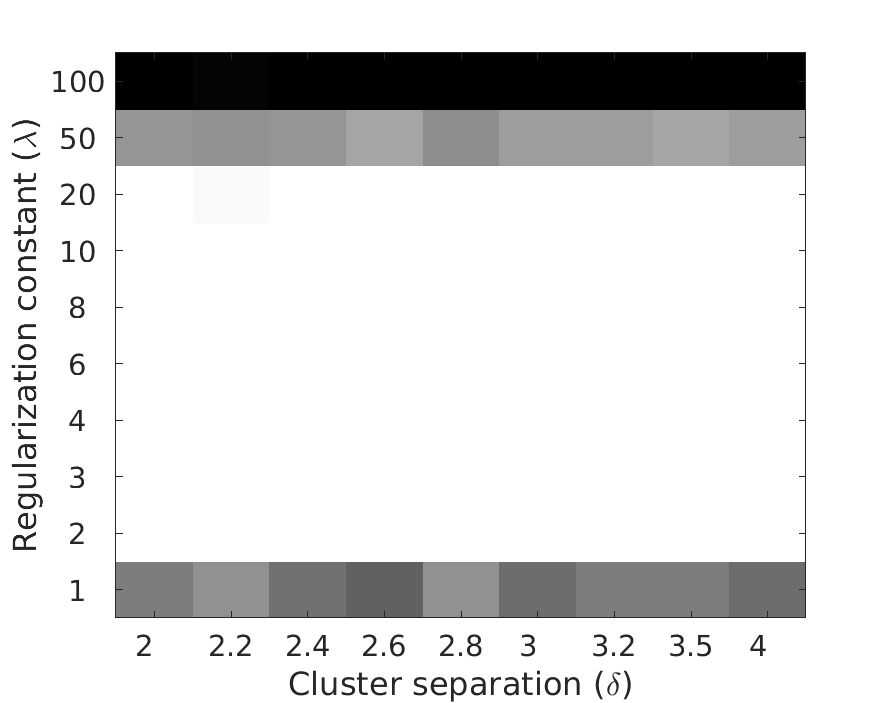
\includegraphics[width=0.4\textwidth]{figures/optimizationClustering/deltaLambda.png}
  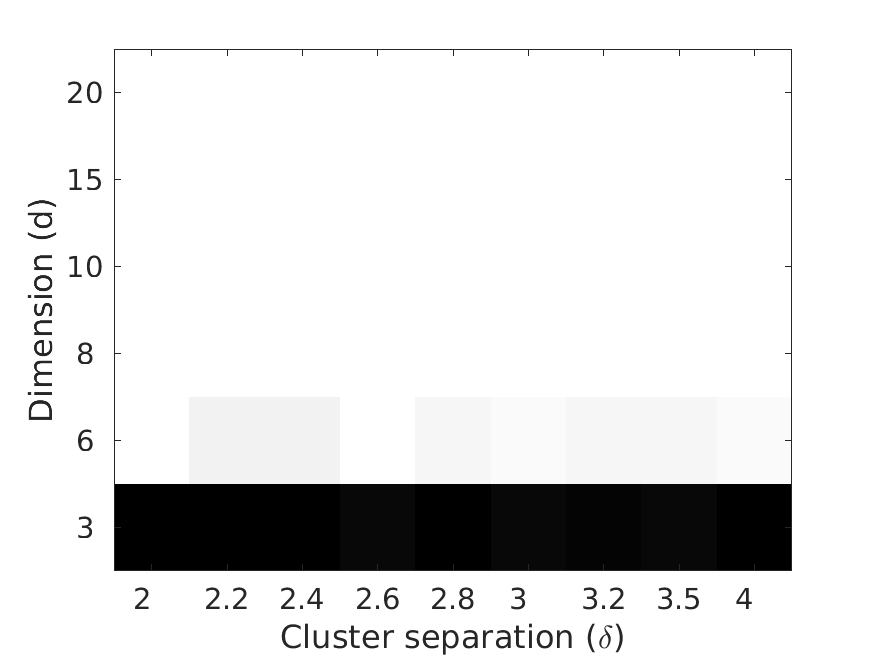
\includegraphics[width=0.4\textwidth]{figures/optimizationClustering/deltaD.png}
  \caption{Heatmap showing the probability of success of the $k$-means regularised sdp algorithm. Lighter color indicates probability closer to one while darker indicates probability closer to zero.}  
\end{figure}

\subsection{Results on MNIST dataset}
We compare our regularised SDP algorithm against $k$-means++ on the MNIST dataset. MNIST is a dataset of images of handwritten digits from zero to nine. It contains 60,000 training images and 10,000 test images. We choose $k = 4$ different classes and randomly sample a total of $N = 1,000$ images from these classes.  We then run both our regularised SDP algorithm and the $k$-means++ algorithm on this dataset. We repeat this process for 10 different random samples of MNIST. We measure the performance of the two algorithms in terms of the precision and recall over the pairs of points in the same cluster. Given a clustering $\mc C$ and some target clustering $C^*$. Define the precision $p$ of $\mc C$ as the fraction of pairs that were in the same cluster according to $\mc C^*$ given that they were in the same cluster according to $\mc C$. The recall $r$ of $\mc C$ is the fraction of pairs that were in the same clustering according to $\mc C$ given that they were in the same cluster according to $\mc C^*$. We finally measure the $f_1$ score of the clustering $\mc C$ as the harmonic mean of its precision and recall. $f_1 = \frac{2pr}{p+r}$. 

Note that the regularised algorithm outputs $k+1$ clusters. Hence, to make a fair comparison, we finally assign each point in the noisy cluster ($C_{k+1}$) to one of the clusters $C_1, \ldots, C_k$ depending upon the distance of the point to the clusters. Another point is that the $f_1$ measures are sensitive to the choice of the $k$ digits or classes. For some choice of $k$ classes, the $f_1$ measures for both the algorithms are higher than compared to other classes. This shows that some classes are more difficult to cluster than other classes. Hence, we only report the difference in performance of the two algorithms. 

We report the performance on datasets with and without noisy points. The first is when there are no outliers or noisy points. In this case, the difference in the $f_1$ values was about $4.34\%$ in favor of $k$-means++. We then added noisy points to the dataset. In the first case, we added images from different datasets like EMNIST (images of handwritten letters). In this case, the difference was $2.54\%$ in favor of the regularised algorithm. In the second case, besides images from different datasets, we also added a few random noisy points to the MNIST dataset. In this case, the difference increased further to about $6.9\%$ in favor of the regularised algorithm. 

\section{Conclusion}
We introduced a regularisation paradigm which can transform any center-based clustering objective to one that is more robust to the addition of noisy points.  We proved that regularised objective is NP-Hard for common cost functions like $k$-means. We then obtained regularised versions of an existing clustering algorithm based on convex (sdp) relaxation of the $k$-means cost. We then proved noise robustness guarentees for the regularised algorithm. The proof improved existing bounds (in terms of cluster separation) for sdp-based standard (non-regularised) $k$-means algorithm. Our experiments showed that regularised sdp-based $k$-means performed better than existing algorithms like $k$-means++ on MNIST especially in the presence of noisy points.
 

\ifdefined\COMPLETE
\else
\end{document}
\fi


\begin{subappendices}
\section{Hardness of regularised $k$-means}
\label{a-section:hardness}
\begin{theorem}
\label{a-theorem:hardFork1Fixed}
Given a clustering instance $\mc X \subset \mb R^{d}$, define $m(\mc X) := \min_{x \neq y \in \mc X} \|x-y\|_{2}^2$ and $n := |\mc X|$. Finding the optimal solution to the regularised $1$-means objective is NP-Hard for $\frac{m(\mc X)}{2} < \lambda < \frac{m(\mc X)}{2} + \frac{1}{2n^2(n-1)}$. 

In particular, the optimization problem is NP-Hard for $\lambda = \lambda_0(\mc X) := \frac{m(\mc X)}{2} + \frac{1}{4n^3}$.
\end{theorem}

\begin{proof}
The proof uses reduction from the clique problem. Given a graph $G = (V, E)$ and an integer $q$, the clique problem asks the following: does there exist a clique in $G$ of size at least $q$?

Given an instance of the clique problem, we construct an instance of regularised $1$-means as follows. For every $v \in V$, construct $x_v \in \mc X$. Define the metric as 
\[
d^2(x_i, x_j) = 
\begin{cases}
1 \hspace{0.51in}\text{if }(i, j) \in E\\
1 + \Delta \hspace{0.221in}\text{if }(i, j) \not\in E\numberthis\label{a-eqn:dmetric}
\end{cases}
\]
where $0 < n\Delta < 1 $. Now, we will show that $G$ has a clique of size $ \ge q$ $\iff$$\mc X$ has a clustering of cost $\le c = \frac{q-1}{4} + \lambda (n - q)$.

$\Longrightarrow$ Assume $G$ has a clique of size at least $q$. Assign all points in the clique to $C_1$ and the remaining points to $C_2$. This clustering has cost as desired.

$\Longleftarrow$ Let $|C_1| = n'$. Now, there are three possibilities.

Case 1: $n' > q$. If all the distances in $C_1$ are 1, then the cost of the clustering is $\frac{n'-1}{4} + \lambda (n - n') \le c$ as $\lambda > \frac{1}{2}$. Thus, the vertices corresponding to the points in $C_1$ form a clique of size $n' > q$. If at least one distance is $1 + \Delta$ then the cost of the clustering is 
\begin{flalign*}
\frac{n'-1}{4} + \lambda (n - n') + \frac{\Delta}{n'} \le c \implies \lambda \ge \frac{1}{2} + \frac{\Delta}{n'(n'-q)}
\end{flalign*}
This is a contradiction because of the choice of $\lambda$.

Case 2: $n' < q$. If all the distances in $C_1 = 1$, then the cost of the clustering is $\frac{n'-1}{2} + \lambda (n - n') > c$. If atleast one distance is $1 + \Delta$ then the cost of the clustering is even greater as $\lambda > \frac{1}{2}$. 

Case 3: $n' = q$. If atleast one distance is $1 + \Delta$ then the cost of the clustering is $\frac{q-1}{2} + \lambda (n - q) + \frac{\Delta}{m} > c$ . 
Hence, the only possibility remains that $|C_1| = q$ and all the distances in $C_1 = 1$. Hence, $G$ has a clique of size $q$.
\end{proof}

\begin{lemma}
Let $d$ be as in Eqn. \ref{a-eqn:dmetric}. Then $d$ can be embedded into $\mb R^{|\mc X|}$.
\end{lemma}
\begin{proof}
The proof of embedding is very similar to Thm. 8 in \cite{dasgupta2008hardness}. Using Cor. 7 in \cite{dasgupta2008hardness}, we know that $D$ can be embedded into $\mb R^{|\mc X|}$ if and only if $u^TDu \le 0$ for all $u^T1 = 0$.
\begin{align*}
u^TDu &= \sum_{ij} u_{i}d_{ij}u_{j} = \sum_{ij}u_iu_j \Big(1 - \mb 1(i=j) + \Delta \mb 1(i \not\sim_{E} j) \big)\\
&\le \Big(\sum_{i}u_i \Big)^2 - \sum_i u_i^2 +\Delta\sum_{ij}|u_i||u_j| \le -\|u\|^2 + |\mc X|\Delta \|u\|^2 = -(1-|\mc X|\Delta)\|u\|^2,
\end{align*}
which completes our proof.
\end{proof}

We now use Thm. \ref{a-theorem:hardFork1Fixed} to show that regularised $1$-means is Np-Hard for any $\lambda > m(\mc X) / 2$.

\begin{restatable}{theorem}{hardForkone}
\label{a-theorem:hardFork1}
Given a clustering instance $\mc X \subset \mb R^d$. Finding the optimal solution to the regularised $1$-means objective is NP-Hard for all $\lambda > m(\mc X) / 2$.
\end{restatable}
\begin{proof}
Denote $d(x,y)$ to be the $l_2$ distance. Thm. \ref{a-theorem:hardFork1Fixed} showed that optimizing the problem  
\begin{align*}
\min_{C\subseteq \mc X} \enspace \sum_{x \in C}d^2(x, c) + \lambda_0(\mc X) \enspace |\mc X\setminus \mc C| \hspace{0.5in}\text{(FRM)}
\end{align*}
is NP-Hard when $\lambda_0(\mc X) := \frac{m(\mc X)}{2} +\frac{1}{4n^3}$. Given $\lambda>0$, we want to show that for all $\lambda > m(\mc X) / 2$, the following is also NP-Hard to optimize: 
\begin{align*}
\min_{C\subseteq \mc X} \enspace \sum_{x \in C}d^2(x, c) + \lambda \enspace |\mc X\setminus \mc C| \hspace{0.5in}\text{(GRM)}
\end{align*}

Let $\lambda' = \sqrt{n^3(4\lambda - 2m(\mc X))} > 0$, and define a new Euclidean distance $d'(x, y) = \frac{d(x,y)}{\lambda'}$. Then
\begin{flalign*}
\sum_{x \in C}d^2(x, c) + \lambda \enspace |\mc X\setminus \mc C| &= \lambda'^2\Bigg(\sum_C d'^2(x, c) + \frac{|\mc X \setminus \mc C|}{\lambda'^2} \Big(\frac{m(\mc X)}{2} +\frac{\lambda'^2}{4n^3}\Big)\Bigg)\\
&= \lambda'^2\Big(\sum_C d'^2(x, c) + |\mc X \setminus \mc C| \lambda_0(\mc X')\Big).&
\end{flalign*}
Hence, we see that GRM is equivalent to FRM which is NP-Hard.
\end{proof}

\section{The regularised $k$-means algorithm}
\label{a-section:heuristic}
 
\subsubsection{Equivalence of regularised $k$-means with $0,1$-SDP}
\label{a-subsection:modifiedkmeans01sdp}
We follow a similar technique to that of \cite{peng2007approximating} to translate equation \ref{eqn:modifiedkmeans} into a 0-1 SDP. We are given a set $\mc X$ with $n$ data points. The goal is to partition the set into $k$ clusters with the option of throwing some points into the garbage $k+1$ cluster. Let $S$ be an assignment matrix of size $n\times k$ and $y$ be an $n \times 1$ column vector that assigns points to the ``garbage'' cluster.  

 \[s_{ij} = 
    \begin{dcases}
		\hspace{0.1in} 1 \enspace \text{iff }x_i \in C_j, j \leq k\\
		\hspace{0.1in} 0 \enspace \text{otherwise}
	\end{dcases}
 \quad y_{i} = 
    \begin{dcases}
		\hspace{0.1in} 1 \enspace \text{iff }x_i \in C_{k+1}\\
		\hspace{0.1in} 0 \enspace \text{otherwise}
	\end{dcases}
\]

Provided that $C_i\ne\emptyset$, we have the following equality by expanding the mean $c_i = \frac{1}{|C_i|} \sum_{x\in C_i} x$:
\begin{align}
\label{a-eqn:kmeansobj1}
\sum_{x \in C_i} \|x-c_i\|^2 
&= \frac{1}{2|C_i|}\sum_{x, y \in C_i} \|x-y\|^2 
\end{align}

\noindent $c_j = \frac{\sum_{i} s_{ij} x_i}{\sum_{i} s_{ij}}$ is the average of points in the $j^{\text{th}}$ cluster. Hence,
\begin{align*}
	&\sum_j \sum_i s_{ij}(\langle c_j, c_j\rangle -2\langle x_i, c_j\rangle) = 	 \sum_j \langle\sum_i s_{ij} c_j, \enspace c_j\rangle - 2 \sum_j \langle\sum_i s_{ij} x_i, \enspace c_j\rangle \\
	&=\sum_j \langle c_j, \sum_i s_{ij}x_i\rangle - 2 \sum_j \langle\sum_i s_{ij} x_i, \enspace c_j\rangle = -\sum_j \langle\frac{\sum_i s_{ij} x_i}{\sum_i s_{ij}}, \sum_i s_{ij}x_i\rangle = -\sum_j \frac{\| \sum_i s_{ij} x_i\|^2}{\sum_i s_{ij}} \numberthis \label{a-eqn:kmeansobj2}
\end{align*}

\noindent Combining equations \ref{a-eqn:kmeansobj1} and \ref{a-eqn:kmeansobj2}, we get that 
\begin{align*}
  &\sum_{j=1}^k \sum_{x \in C_i} \|x-c_i\|^2 = \sum_{i=1}^n \|x_i\|^2 (1-y_i) - \sum_{j=1}^k \frac{\| \sum_i s_{ij} x_i\|^2}{\sum_i s_{ij}} = \sum_{i=1}^n \|x_i\|^2 (1-y_i) - \sum_{i=1}^n\sum_{j=1}^n \langle x_i, x_j\rangle Z_{ij} \label{a-eqn:halfcost}\numberthis
\end{align*}

where $Z = S (S^T S)^{-1} S^T$. Observe that if $x_i \not\in C_{k+1}$ then $Z_{ij} = \frac{1}{|S_{c(i)}|} \langle s_i, s_j\rangle$ where $S_{c(i)}$ denotes the size of the $i^{th}$ cluster. If $x_i \in C_{k+1}$ then $Z_{ij}=0$. Thus, 
\[
	Z_{ij} = 
	\begin{dcases}
	\frac{1}{|S_{c(i)}|} \langle s_i, s_j\rangle \quad &\text{if }y_i = 0\\
	0 \quad &\text{otherwise }
	\end{dcases}
\]
Observe that $Z_{ij} = Z_{ji}$ and
\begin{align*}
\tr(Z) &= \sum_i Z_{ii} = \sum_{x \not\in C_{k+1}} \frac{1}{|S_{c(i)}|} = k. 
\end{align*}
Also, we have that  and $\langle Z_i, \mb 1\rangle = \sum_{j} Z_{ij}$. If $y_i = 0$ then $\sum_{j}Z_{ij} = 0$ else $\sum_j Z_{ij} = \frac{1}{|S_{c(i)}|}\sum_j \langle s_i, s_j\rangle = 1$. Hence, we get that $\langle Z_i, \mb 1\rangle = \sum_j Z_{ij} = 1-y_i$, or equivalently, $Z\cdot \mb 1 + y = \mb 1$. Also, it is fairly easy to see that $Z^2 = Z$.

Let $D$ be a matrix such that $D_{ij} = d^2(x_i, x_j)$. Using the above properties of $Z$, we get that
\begin{align*}
&\tr(DZ) = \sum_{ij} \langle x_i - x_j, x_i-x_j\rangle z_{ij} = \sum_i\|x_i\|^2\sum_j z_{ij} + \sum_j\|x_j\|^2\sum_i z_{ij} -2\sum_{ij}\langle x_i, x_j\rangle z_{ij} \\
&= 2\Big( \sum_i\|x_i\|^2 (1-y_i) - \sum_{ij}\langle x_i, x_j\rangle z_{ij}\Big) = 2 \sum_{i=1}^k \sum_{x \in C_i} \|x-c_i\|^2 \text{ (using Eqn. \ref{a-eqn:halfcost})}
\end{align*}

Finally, observe that $\lambda |C_{k+1}| = \lambda\langle \mb 1, y\rangle$.

\begin{equation*}
	\begin{split}
	\textbf{0-1}\\
	\textbf{SDP}
  \end{split}
	\begin{cases}
		\min_{Z, y} \enspace &\tr(DZ) + \lambda \langle \mb 1, y\rangle\\
		\text{s.t. } \enspace &\tr(Z) = k\\
		& Z\cdot \mb 1 + y = \mb 1\\	
		&Z\ge 0, Z^2 = Z, Z^T = Z \\
		& y \in \{0, 1\}^n
	\end{cases}
	\xrightarrow{\text{relaxed}} \textbf{ SDP } 
	\begin{cases}
		\min_{Z, y} \enspace &\tr(DZ) + \lambda \langle \mb 1, y\rangle\\
        \text{s.t. } \enspace &\tr(Z) = k\\
		& \Big(\frac{Z+Z^T}{2}\Big)\cdot \mb 1 + y = \mb 1\\		
		&Z \ge 0, y \ge 0, Z \succeq 0 \numberthis\label{a-eqn:regularisedSDP}
	\end{cases}
\end{equation*}

\begin{restatable}{theorem}{modifiedkmeans}
\label{a-thm:modifiedkmeans}
Finding a solution to the 0-1 SDP (\ref{eqn:regularisedSDP}) is equivalent to finding a solution to the regularised $k$-means objective (\ref{eqn:modifiedkmeans}). 
\end{restatable}

\begin{proof}
We will use the same proof ideas as in the proof of Theorem 2.2 in \cite{peng2007approximating}. However, we need to modify the proof slightly according to our formulation. From the discussion in the previous subsection, we can see that any solution for (\ref{eqn:modifiedkmeans}) implies a solution for the 0-1 SDP (\ref{eqn:regularisedSDP}) with same cost. Now, we will prove the other direction. Any solution for the 0-1 SDP implies a solution for for (\ref{eqn:modifiedkmeans}) with same cost.

Let $e_i$ be a vector with all zeros except in the $i^{\text{th}}$ index. Observe that $u_i^T Z u_i \ge 0$. Hence, $Z_{ii} \ge 0$. Similarly, $(e_i-e_j)^T Z (e_i-e_j) = Z_{ii} - 2Z_{ij} + Z_{jj}$. Hence, $Z_{ij} \le \max (Z_{ii}, Z_{jj})$. Let $Z_{i^*i^*} = \max_i Z_{ii}$. Hence, we have that for all $i, j$, $Z_{ij} \le Z_{i^* i^*}$. 

Suppose $Z_{i^*i^*} = 0$. Then, $Z = \textbf{0}$ and $y = \textbf{1}$. This implies that all points are assigned to the $k+1$ cluster. The cost of both the solutions in this case is $\lambda |C_{k+1}|$.

Now, suppose $Z_{i^*i^*}>0$. Let $I =\{j: Z_{i^* j} > 0\}$. Since, $Z^2 = Z$, we have that $Z_{i^*i^*} = \sum_{j=1}^n Z^2_{i^* j} = \sum_{j \in I} Z^2_{i^*j}$. Hence, $\sum_{j \in I}\frac{Z_{i^*j}}{Z_{i^*i^*}}Z_{i^*, j} = 1$. Also, we have that $\sum_{j} Z_{i^*j} + y_{i^*} = 1$. If $y_{i^*} = 1$, then $\sum_{j} Z_{i^*j} = 0$ which contradicts our assumption that $Z_{i^*i^*} > 0$. Hence, $y_{i^*} = 0$ and we have $\sum_{j} Z_{i^*j} = \sum_{j\in I} Z_{i^*j} = 1$. Since we have the following constraints,
\begin{align*}
	\sum_{j\in I} Z_{i^*j} = 1 \hspace{0.4in}\text{and} \hspace{0.4in}\sum_{j\in I} \frac{Z_{i^*j}}{Z_{i^*i^*}}Z_{i^*j} = 1
\end{align*}
$Z_{i^*j} = Z_{i^*i^*}$ for all $j \in I$. Hence, we see that the matrix $Z$ and the vector $y$ can be decomposed as 
\[ Z = 
\begin{bmatrix}
    Z_{II}  & 0 \\
    0       & Z'
\end{bmatrix}
\quad y=\begin{bmatrix}
    0 \\
    y' 
\end{bmatrix}
\]
where $Z_{II} = \frac{1}{|I|}\mb1_{|I|}\mb1_{|I|}^T$. Now, we can see that $\tr(Z') = k-1$ and
$$Z\mb 1 + a = \begin{bmatrix}1\\Z'\mb 1\end{bmatrix} + \begin{bmatrix}0\\a'\end{bmatrix} = \begin{bmatrix}1\\1\end{bmatrix}.$$

This implies that $Z'\cdot \mb 1 + y' = \textbf{1}$. Hence, the optimization problem now reduces to
 \[
    \begin{cases}
		\min_{Z',y'} \enspace &\tr(DZ') + \lambda\langle \cdot \mb 1, y'\rangle\\
		\text{subject to } \enspace &\tr(Z') = k-1\\
		&Z'\cdot \mb 1 + y' = \mb 1
	\end{cases}
\]
Repeating this process $k$ times, we get that $Z$ can be decomposed into $k$ non-zero block diagonal matrices and one zero block diagonal matrix. Hence, using this we construct a solution for the original clustering problem as follows. For all $i$, if the row $Z_i$ belongs to the $j^{th}$ diagonal block then $x_i$ is assigned to $C_i$. Given $Z$ and $a$, the cost of the 0-1 SDP solution is
\begin{align*}
\frac{1}{2} \tr(DZ) + \lambda\langle\mb 1, y\rangle &= \sum_{i=1}^k\sum_{x,y \in C_i} \frac{\|x_i-x_j\|^2}{2|C_i|} + \lambda|C_{k+1}| = \sum_{i=1}^k \sum_{x \in C_i} \|x-c_i\|^2 + \lambda |C_{k+1}|
\end{align*}
which is the same as the cost of the regularised $k$-means objective. Hence, from a feasible solution of (\ref{eqn:modifiedkmeans}), we can obtain a feasible solution of the 0-1 SDP of same cost.
\end{proof}

\section{Tightness of the SDP based algorithm}
\begin{equation*}
	\textbf{0-1 SDP} 
	\begin{cases}
		\min_{Z} \enspace &\tr(DZ) \\
		\text{subject to } \enspace &\tr(Z) = k\\
		& Z\cdot \mb 1 = \mb 1\\	
		&Z\ge 0, Z^2 = Z, Z^T = Z 
	\end{cases}
	\xrightarrow{\text{relaxed}} \textbf{ SDP } 
	\begin{cases}
		\min_{Z} \enspace &\tr(DZ)\\
        \text{subject to } \enspace &\tr(Z) = k\\
		& \Big(\frac{Z+Z^T}{2}\Big)\cdot \mb 1 = \mb 1\\		
		&Z \ge 0, Z \succeq 0 \numberthis\label{a-eqn:SDP}
	\end{cases}
\end{equation*}

We are given a set $\mc X \subset \mb R^d$. $\mc X$ can be covered by a set of $k$ ``well-separated'' balls. That is, $\mc X := \cup_{i=1}^k B_i$ where $B_i$ is a ball of radius at most $r$ centered at $\mu_i$ and $\|\mu_i - \mu_j\| \ge \delta r$. %Let $\mc P$ denote the isotropic distribution in the unit ball centered at origin $B_1(r)$ in $\mb R^d$. The ball $B_i$ is drawn from the isotropic distribution $\mc P_i$, that is, the measure $\mc P$ translated with respect to the center $\mu_i$. 
Define $n_i := |B_i|$ and $n := \min_{i\in[k]} n_i$ and $N = \sum_i n_i$. $D$ is an $N\times N$ matrix such that $D_{ij} = \|x_i -x_j\|^2$.  

The goal is to output a clustering $\mc C^*$ of $\mc X$ such that $C^* = \{B_1, B_2, \ldots, B_k\}$. From the way we constructed the 0-1 SDP, this corresponds to
\begin{align}
  Z^* = \sum_{p=1}^k \frac{\mb 1^p \mb 1^{p^T}}{n_p} \label{a-eqn:intendedsolution}
\end{align}
where $\mb 1^p$ is an $N$-dimensional indicator vector for the $p^{th}$ cluster. That is, $Z$ is a block diagonal matrix and consists of $k$ non-zero diagonal blocks. Observe that $Z$ consists of blocks $Z^{(p, q)}$. Also, $Z^{(p, p)} = \frac{1}{n_p}\mb 1\mb 1^T$ and for $p \neq q, Z^{(p, q)} = 0$. To prove that our SDP (Eqn. \ref{a-eqn:SDP}) finds this solution, we  will adopt the following strategy. We first construct a dual for Eqn. \ref{a-eqn:SDP}. We then show that under certain conditions on $\delta$ (well-separateness of the balls) the following happens. The primal objective value and the dual objective value are the same. Also, the corresponding $Z$ satisfies Eqn. \ref{a-eqn:intendedsolution}. 

Before, we describe the dual, lets introduce a bit of notation. We index every point as $(p, i)$ where $p$ denotes the ball (or cluster) to which it belongs and $i$ denotes the index within that ball. Observe that the distance matrix $D$ consists of blocks $D^{(p, q)}$ such that $D^{(p,q)}_{ij} = \|x_{(p,i)}-x_{(q,j)}\|^2_2$. Now, to construct the dual, we introduce variables $z, \alpha_{(p,i)}, \beta_{(p,i)(q,j)}$ and $Q$ for each of the constraints in the primal problem. 
\[\textbf{SDP Dual}
    \begin{cases}
		\max \enspace &-zk - \sum_{p=1}^{k}\sum_{i=1}^{n_p} \alpha_{(p,i)}\\
		\text{subject to } \\
		&Q = D + zI + \sum_p\sum_i \alpha_{(p,i)}A_{(p, i)} -\sum_{p,q}\sum_{i,j} \beta_{(p,i)(q,j)}E_{(p,i)(q,j)}\\
		&\beta \ge 0 \\
		&Q \succeq 0
	\end{cases}
	\label{a-eqn:SDPDual}
	\numberthis
\]
where, $A_{(p,i)} = \frac{1}{2}(e_{p,i}\mb 1^T + \mb 1 e_{p, i}^T)$ and $E_{(p,i)(q,j)} = e_{(p,i)}e_{(q,j)}^T$. $\mb 1$ is an $N$-dimensional vector of all ones while $e_{p,i}$ is the indicator vector with one in position $(p, i)$ and zeros elsewhere. Now, we will examine the conditions under which the dual objective value matches the primal objective such that all the constraints of the dual are satisfied. 
\subsubsection*{Complementary slackness}
We know that $\beta_{(p, i)(q, j)} Z_{(p, i)(q, j)} = 0$. Now, $Z^{(p, q)} = 0$ and $Z^{(p, p) \neq 0}$. Hence, we get that $\beta^{(p, p)} = 0$. Also, if we have that $Q^{(p,p)}\mb1 = 0$ then $\langle Q, Z \rangle = 0$. This ensures that the second complementary slackness condition is also satisfied. 

\subsubsection*{Some properties of the $Q$ matrix}
Before we proceed, let's examine some properties of the dual matrix $Q$. Observe that for all $1 \le p\neq q \le k$, 
\begin{alignat*}{1}
&Q^{(p,p)} = D^{(p,p)} + zI_{n_p} + \frac{1}{2}\sum_{i=1}^{n_p} \alpha_{(p,i)} (e_{i}\mb 1^T + \mb 1e_{i}^T)\\
&Q^{(p,q)} = D^{(p,q)} + \frac{1}{2}\sum_{i=1}^{n_p} \alpha_{(p,i)} e_{i}\mb 1^T + \frac{1}{2}\sum_{i=1}^{n_q}\alpha_{(q,i)}\mb 1e_{i}^T - \beta^{(p,q)}
\label{a-eqn:q}\numberthis
\end{alignat*} 

\subsubsection*{Dual matches intended primal solution}
Now, using the fact that $Q^{(p, p)}\mb 1 = 0$ implies that
\begin{align*}
  0 &= e_r^TD^{(p,p)}\mb1 + z + \frac{1}{2}\sum\alpha_{(p,i)} (e_r^Te_{i}\mb 1^T\mb1 + \mb e_r^T\mb1e_{i}^T\mb1) = e_r^TD^{(p,p)}\mb1 + z\\
  & + \frac{1}{2}\sum\alpha_{(p,i)} (e_r^Te_{i}n_p + 1) = e_r^TD^{(p,p)}\mb1 + z + \frac{1}{2}\sum\alpha_{(p,i)} +\frac{n_p\alpha_{(p,r)}}{2}.
\end{align*}
Summing over all $r$ and then substituiting back, we get that for all $1\le p \le k$ and for all $i$,  
\begin{align*}
  &\alpha_{(p, i)} = \frac{1^TD^{(p,p)}1}{n_p^2}-\frac{z}{n_p} -\frac{2e_i^TD^{(p,p)}1}{n_p}\\
  & = \frac{\sum_{i,j}\langle x_{pi}-x_{pj}, x_{pi}-x_{pj}\rangle -2n_p \sum_j\langle x_{pi}-x_{pj}, x_{pi}-x_{pj}\rangle}{n_p^2}-\frac{z}{n_p}\\
  &= \frac{-2n_p^2 \|x_{pi}\|^2 + 4n_p \langle x_{pi}, \sum_jx_{pj}\rangle - 2\langle \sum_i x_{pi}, \sum_j x_{pj}\rangle -zn_p}{n_p^2}\\
  &= -2\|x_{pi} - x_p\|^2-\frac{z}{n_p} \hspace{1in}\text{ ($x_p$ denotes the center of the $p^th$ cluster)}\numberthis \label{a-eqn:alphapi}
\end{align*}
Now, we have the value of $\alpha$ for all $1\le p \le k$ and for all $i$. Computing the objective function, we get that 
\begin{align*}
  kz + \sum_p\sum_i \alpha_{p,i} &= kz + \sum_{p}\frac{1^TD^{(p, p)}1}{n_p} - \sum_p z -2\sum_p \frac{1^TD^{(p,p)}1}{n_p} = -\sum_p \frac{\mb1^TD^{(a,a)}\mb1}{n_p}\\
  & = -\langle D, Z \rangle = -\tr(DZ)
\end{align*}
Hence, we see that for the intended solution, the primal and dual values are the same. Hence, solution is optimal. Now, the main question is to find $Q$ such that $Q$ is positive semi-definite while simultaneously ensuring that $\beta \ge 0$.  

\subsubsection*{Satisfying PSD for $Q$}
We already know that $Q^{(p,p)}\mb 1 = 0$. We will now try to ensure that $Q^{(p, q)}\mb 1 = 0$. As we will see later, this will help us to prove the positive semi-definiteness property for $Q$. Now, $Q^{(p,q)}1 = 0$ implies that for all $r$, we have $e_r^TQ^{(p,q)}1 = 0$.  
\begin{flalign*}
  &0 = e_r^TQ^{(p, q)}1 = \sum_s Q^{(p,q)}_{rs} = \sum_{s} D^{(p, q)}_{rs} + \frac{n_q \alpha_{(p,r)}}{2} + \frac{1}{2}\sum_{i=1}^{n_q}\alpha_{(q, i)} - \sum_{s}\beta^{(p, q)}_{rs}&
\end{flalign*}
It is always possible to satisfy the above equation by choosing $\beta_{rs}^{(p,q)}$ as long as it is greater than zero. That is we need that, 
\begin{align*}
  &\beta^{(p,q)}_{rs}  := \frac{\sum_{s} D^{(p, q)}_{rs}}{n_q} + \frac{\alpha_{(p,r)}}{2} + \frac{\sum_{i=1}^{n_q}\alpha_{(q, i)}}{2n_q} \ge 0\\
  &\iff \frac{\sum_{s} \|x_{pr}-x_{qs}\|^2}{n_q} \ge \frac{\sum_s\|x_{qs} - x_q\|^2}{n_q} + \|x_{pr} - x_p\|^2 + \frac{z}{2n_p} + \frac{z}{2n_q} \numberthis \label{a-eqn:qpq1tmp}
\end{align*}
Before, we go further lets examine,
\begin{align*}
  &\sum_{s} \|x_{pr}-x_{qs}\|^2 = n_q\|x_{pr}\|^2 - 2n_q\langle x_{pr}, x_q \rangle + \sum_s \|x_{qs}\|^2\\
  & = n_q \|x_{pr}-x_q\|^2 + \sum_s \langle x_{qs}, x_{qs}\rangle - n_q\langle x_q, x_q \rangle = n_q \|x_{pr}-x_q\|^2 + \sum_s \|x_{qs} - x_q \|^2
\end{align*} 
Substituting this in Eqn. \ref{a-eqn:qpq1tmp}, we get that it is always possible to satisfy $Q^{(p, q)}1 = 0$ as long as for all $r$, we have that 
\begin{align}
  \|x_{pr} - x_q\|^2 - \|x_{pr} - x_p\|^2 \ge \frac{z}{2n_p} + \frac{z}{2n_q}\label{a-eqn:zupper}
\end{align}
Also, note that from $\beta_{rs}^{(p,q)}$ as defined in Eqn. \ref{a-eqn:qpq1tmp}, we get that 
\begin{align}
  &Q_{rs}^{(p,q)} = D^{(p, q)}_{r,s} + \frac{1}{2}\alpha_{q, s} - \frac{1}{n_q}\sum_j D^{pq}_{rj} -\frac{1}{2}\frac{\sum_j \alpha_{qj}}{n_q} \hspace{0.3in}\text{ and from Eqn. \ref{a-eqn:q}}\\
  &Q_{rs}^{(p,p)} = D^{(p, p)}_{r,s} + \frac{1}{2}\alpha_{p, r} + \frac{1}{2}\alpha_{p, s} + z \mb 1_{[r=s]}
\end{align}
If Eqn.\ref{a-eqn:zupper} holds, then for all $1 \le p, q \le k$, we have that $Q^{(p,q)}\mb1 = 0$. Let $\mb 1_p$ denote the $N$-dimensional indicator vector for the $p^{th}$ cluster. Then, we see that for all $1 \le p \le k$, we have that $Q \mb 1_p = 0$. Let $V$ be the subspace spanned by these vectors. That is, $V = span\{1_p\}_{p=1}^k$. Then, for all $v \in V$, $v^T Q y = v^T \mb 0 = \mb 0$. Hence, we need to only show that for all $v \bot V$, $v^TQv \ge 0$. Let $v = [v_1, \ldots, v_k]^T$. Since, $v \bot V$, we know that for all $p$, $\langle v_p, 1\rangle = 0 = \sum_{r}v_{pr}$. Now,
\begin{align*}
  &v^TQv = \sum_{pq}\sum_{rs}x_{pr}Q^{(p, q)}_{rs}v_{qs} = \sum_{p \neq q}\sum_{rs}v_{pr}Q^{(p, q)}_{rs}v_{qs} + \sum_{p}\sum_{rs}v_{pr}Q^{(p, p)}_{rs}v_{qs}
\end{align*}
Now, we analyse the case when $p \neq q$. Then, we have that
\begin{align*}
  &\sum_{rs}v_{pr}Q^{pq}_{rs}v_{qs} = \sum_{rs}v_{pr}D^{pq}_{rs}v_{qs} + \frac{1}{2}\sum_{rs}\alpha_{qs}v_{qs}v_{pr} -\frac{1}{n_q}\sum_{rs} \sum_j v_{pr}v_{qs}D^{pq}_{rj} -\frac{1}{2n_q}\sum_{rs}\sum_jv_{pr}v_{qs}\alpha_{qj}\\
  &= \sum_{rs}v_{pr}v_{qs}D^{pq}_{rs} + \frac{1}{2}\sum_{s}\alpha_{qs}v_{qs}\sum_r v_{pr} -\frac{1}{n_q}\sum_{r}\sum_j D^{pq}_{rj}v_{pr}\sum_sv_{qs} -\frac{1}{2n_q}\sum_{s}\sum_jv_{qs}\alpha_{qj}\sum_{r}v_{pr}\\
  &= \sum_{rs}v_{pr}v_{qs}D^{pq}_{rs}
\end{align*}
Now for the other case, we have that
\begin{align*}
  \sum_{rs}v_{pr}Q^{pp}_{rs}v_{ps} &= \sum_{rs}v_{pr}D^{pp}_{rs}v_{ps} + \frac{1}{2}\sum_{rs}\alpha_{pr}v_{pr}v_{ps} + \frac{1}{2}\sum_{rs}\alpha_{ps}v_{pr}v_{ps} + \sum_r zv_{pr}v_{pr}\\
  &= \sum_{rs}v_{pr}D^{pp}_{rs}v_{ps} + \frac{1}{2}\sum_{r}\alpha_{pr}v_{pr}\sum_sv_{ps} + \frac{1}{2}\sum_{s}\alpha_{ps}v_{ps}\sum_r v_{pr} + \sum_r zv_{pr}v_{pr}\\
  &=\sum_{rs}v_{pr}D^{pp}_{rs}v_{ps} + \sum_r zv_{pr}v_{pr}
\end{align*}
Combining the above two equations, we get that 
\begin{align*}
  &v^TQv = \sum_{pq}v_{pr}D^{pq}v_{qs} + z\sum_p\sum_{r} (v_{pr})^2 = v^TDv + zv^Tv
\end{align*}
Now, let $X$ be the $N \times d$ dimensional input matrix. That is, the matrix $X$ contains the $N$ points in $d$ dimensional euclidean space. Then, $D = W + W^T - 2 XX^T$ where $W$ is a rank one matrix such that its $i^{th}$ contains $\|x_i\|^2$ in its $i^{th}$ row. That is, $W = \sum_i \|x_i\|^2 e_i\mb 1^T$. Now, $v \bot V$, hence we get that $v^TDv = -2v^TXX^Tv$. Thus, $Q$ is positive semi-definite as long as we can find $z$ such that  
\begin{align*}
  &z > 2 \max_{v\bot V} \frac{v^T XX^Tv}{v^Tv}. \label{a-eqn:zlower}\numberthis
\end{align*}

\subsubsection*{Putting it all together}
Eqns. \ref{a-eqn:zlower} and \ref{a-eqn:zupper}, show that as long as 
\begin{align}
  \|x_{pr} - x_q\|^2 - \|x_{pr}-x_p\|^2  > \frac{2}{n}\Big(\max_{v\bot V} \frac{v^T XX^Tv}{v^Tv}\Big)\label{a-eqn:mainConstraint}
\end{align}
  then we can find $Q$ and $\beta$ satisfying the constraints of the dual and there is no primal and dual gap. First observe that LHS of Eqn. \ref{a-eqn:mainConstraint} has a minimum of $(\delta - 1)^2 - 1$. Now, we need to upper bound the RHS of Eqn. \ref{a-eqn:mainConstraint}. Note that $X = X' + X$ where $C$ is a rank $k$ matrix which contains the centers $\mu_1, \ldots, \mu_k$. Also, for any $v \bot V$, we have that $v^TC = 0$. Let $\sigma_{\max}$ denote the maximum eigenvalue of the matrix $X$. Hence, 
\begin{align*}
  &\frac{2}{n}\Big(\max_{v\bot V} \frac{v^T XX^Tv}{v^Tv}\Big) = \frac{2}{n}\Big(\max_{v\bot V} \frac{v^T X'X'^Tv}{v^Tv}\Big) \le \frac{2}{n}\sigma_{\max}\big(X'\big)^2\numberthis\label{a-eqn:mainConstrintUpper}
\end{align*}
The last inequality follows from the Defn. of $\sigma_{\max}$. (Eqn. 5.3 in \cite{vershynin2010introduction}). We are now in a position to state our result.
  
\begin{theorem}
\label{a-thm:SDPGeneral}
Given a clustering instance $\mc X \subset \mb R^{N\times d}$ and $k$. Let $\mc X := \cup_{i=1}^k B_i$ where $B_i$ is a finite set of radius at most $r$ centered at $\mu_i$. That is, $B_i = \{x : \|x -\mu_i\| \le r\}$. Furthermore, let $\|\mu_i - \mu_j\| \ge \delta r$ and $ n := \min_{i} |B_i|$. Define $B_i' := \{x - \mu_i : x \in B_i\}.$  and $\mc X' = \cup B_i'$. If 
$$\delta > 1 + \sqrt{1+\frac{2\sigma_{\max}^2(\mc X')}{n}}$$ 
then the $k$-means SDP finds the intended cluster solution  $\mc C^* = \{B_1, \ldots, B_k\}$.
\end{theorem}

Note that Thm. \ref{a-thm:SDPGeneral} doesn't make any assumptions on the distribution that generated the points $\mc X$. In general, the eigenvalues of the matrix $\mc X'$ are bounded by $\sqrt{Nr}$. Let $\rho := \frac{N}{nk}$. $\rho$ measures the balance of the clusters. If all the clusters have the same size then $\rho = 1$. Using this notation, we get the following corollary
 
\begin{corollary}
\label{a-corollary:SDPGeneral}
Given a clustering instance $\mc X \subset \mb R^{N\times d}$ and $k$. Let $\mc X := \cup_{i=1}^k B_i$ where $B_i$ is a finite set of radius at most $r$ centered at $\mu_i$. That is, $B_i = \{x : \|x -\mu_i\| \le r\}$. Furthermore, let $\|\mu_i - \mu_j\| \ge \delta r$. If 
$$\delta > 1 + \sqrt{1+ 2r\rho k}$$ 
then the $k$-means SDP finds the intended cluster solution  $\mc C^* = \{B_1, \ldots, B_k\}$.
\end{corollary}

\noindent Cor. \ref{a-corollary:SDPGeneral} holds for any distribution that generated the data $\mc X$. However, the separation $\delta$ depends on the number of clusters $k$. Next, we show that if the data is generated by an isotropic distribution $\mc P$ then we can get rid of the dependence on $k$ and get the positive results as long as $\delta > 2$. 

In this setting, as before we are given a set $\mc X$ which can be covered by $k$ ``well-separated'' balls. That is, $\mc X := \cup_{i=1}^k B_i$ where each $B_i$ is generated as follows. Let $\mc P$ denote the isotropic distribution on the ball centered at origin of radius atmost $r$, that is $B_1(r)\subset \mb R^d$. Let $B_i$ be a set of $n_i$ points drawn according to $P_i$, the measure $\mc P$ translated to $\mu_i$. Also, $\|\mu_i - \mu_j\| > \delta r > 2r$. 

%We need to ensure that for $\mc X$ as generated above, Eqn. \ref{a-eqn:mainConstraint} can be satisfied.  Consider the set $B_p$. This set has been drawn according to the isometric distribution $\mc P_p$ with mean $\mu_p$. Using Thm. \ref{a-thm:generalizedHoeffding}, we get that if $n_i > c\frac{\log(k/\delta)}{\epsilon^2}$ then with probability atleast $1-\delta/k$ we have that $\|x_p - \mu_p\| \le r^2 \epsilon$. Using a union bound over all $k$ balls, we get that if $n > c\frac{\log(k/\delta)}{\epsilon^2}$ then we hav that for all $p$, $\|x_p-\mu_p\|^2 \le r^2\epsilon$. For remainder of this section, we assume that $r = 1$. 

%Using this, we can now lower bound the LHS of Eqn. \ref{a-eqn:mainConstraint}. 
%\begin{align*}
%  &\|x_{pr} - x_q\|^2 - \|x_{pr} - x_p\|^2 \ge (\|x_{pr} - \mu_q\| - \|x_q - \mu_q\|)^2 - (\|x_{pr} - \mu_p\| + \|x_p - \mu_p\|)^2\\
%  &= \|x_{pr} - \mu_q\|^2 -\|x_{pr} - \mu_p\|^2 +  \|x_q - \mu_q\|^2 - \|x_p - \mu_p\|^2 - 2\|x_{pr} - \mu_p\|\|x_{p} - \mu_p\| - 2\|x_{pr}-\mu_q\|\|x_q-\mu_q\|\\
%  &\ge (\delta-1)^2 - 1 - \epsilon - 4\sqrt{\epsilon}
%\end{align*}

Let $\Theta = E[\|x_{pr}'\|^2]$. Using Thm. \ref{a-thm:spectralNormCOncentration}, we can bound the RHS of Eqn. \ref{a-eqn:mainConstraint} by upper bounding the maximum eigenvalue of $X'$ as 
\begin{align}
  &\mb P\bigg[\sigma_{\max}\bigg(\sqrt{\frac{d}{\theta}}X'\bigg) > \sqrt{N} + t\sqrt{\frac{d}{\theta}} \bigg] \le 2d\exp(-ct^2)
\end{align}

Now, let $t\sqrt{\frac{d}{\theta}} = s\sqrt{N}$. Then, we get that with probability atleast $1-2d\exp(-\frac{c\theta Ns^2}{d})$ we have that 
\begin{align*}
  &\frac{2}{n}\sigma_{\max}(X')^2 \le 2(1+s)^2\frac{N\theta}{nd} \le 2\rho\theta (1+s)^2\frac{1}{d}
\end{align*}

%So we see that as long $(\delta - 1)^2 - 1 > \epsilon + 4\sqrt{\epsilon} + 2k\rho\theta (1+s)^2\frac{1}{d}$, the primal and dual objective value are the same with high probability. In other words $\delta > 2 + {\epsilon + 4\sqrt{\epsilon} + 2k\rho\theta(1+s)^2\frac{1}{d}}$ implies the desired conditions. Now, we are finally ready to state our result.
So we see that as long $(\delta - 1)^2 - 1 > 2k\rho\theta (1+s)^2\frac{1}{d}$, the primal and dual objective value are the same with high probability. In other words $\delta > 1 + \sqrt{1+2\rho\theta(1+s)^2\frac{k}{d}}$ implies the desired conditions. Now, we are finally ready to state our result.

\begin{theorem}
\label{a-thm:SDPIsometric}
Let $\mc P$ denote the isotropic distribution on the ball centered at origin of radius $r$, that is on, $B_1(r)$ in $\mb R^d$. Given centers $\mu_1, \ldots, \mu_k$ such that $\|\mu_i - \mu_j\| > \delta r > 2 r$. Let $\mc P_i$ be the measure $\mc P$ translated with respect to the center $\mu_i$. Given a clustering instance $\mc I := \cup_{i=1}^k B_i$ where each $B_i$ is drawn i.i.d w.r.t $\mc P_i$. If the distance between the centers of any two balls
$$\delta > 1 + \sqrt{1+\frac{2\theta\rho k}{d}\Big(1+\frac{1}{\log N}\Big)^2}$$  
where $\rho = \frac{N}{nk}$ and $ n := \min_{i\in[k]} |B_i|$ and $\theta = \mb E[\|x_{pi}-\mu_p\|] < 1$, then there exists a constant $c > 0$ such that with probability at least $1 - 2d\exp(\frac{-cN\theta}{d\log^2N})$ the $k$-means SDP finds the intended cluster solution  $\mc C^* = \{B_1, \ldots, B_k\}$.
\end{theorem}

\section{Tightness of the regularised SDP based algorithm}
\begin{equation*}
	\textbf{0-1 SDP} 
	\begin{cases}
		\min_{Z, y} \enspace &\tr(DZ) + \lambda \langle \mb 1, y\rangle\\
		\text{subject to } \enspace &\tr(Z) = k\\
		& Z\cdot \mb 1 + y = \mb 1\\	
		&Z\ge 0, Z^2 = Z, Z^T = Z \\
		& y \in \{0, 1\}^n
	\end{cases}
	\xrightarrow{\text{relaxed}} \textbf{ SDP } 
	\begin{cases}
		\min_{Z} \enspace &\tr(DZ) + \lambda \langle \mb 1, y\rangle\\
        \text{subject to } \enspace &\tr(Z) = k\\
		& \Big(\frac{Z+Z^T}{2}\Big)\cdot \mb 1 + y = \mb 1\\		
		&Z \ge 0, y \ge 0, Z \succeq 0 \numberthis\label{a-eqn:regularisedSDP}
	\end{cases}
\end{equation*}

We are given a set $\mc X \subset \mb R^d$. $\mc X = \mc I \cup \mc N$ is such that $\mc I$ can be covered by a set of $k$ ``well-separated'' balls. That is, $\mc I := \cup_{i=1}^k B_i$ where $B_i$ is a ball of radius at most $r$ centered at $\mu_i$ and $\|\mu_i - \mu_j\|_{2}^{2} \ge \delta r$. %Let $\mc P$ denote the isotropic distribution in the unit ball centered at origin $B_1(r)$ in $\mb R^d$. The ball $B_i$ is drawn from the isotropic distribution $\mc P_i$, that is, the measure $\mc P$ translated with respect to the center $\mu_i$. 
Define $n_i := |B_i|$ and $n := \min_{i\in[k]} n_i$ and $m := |\mc N| = n_{k+1}$ and $N = \sum_i n_i + m$. $D$ is an $N\times N$ matrix such that $D_{ij} = \|x_i -x_j\|^2$.  

Note that the clustering algorithm gets $\mc X$ as input and does not know about the sets $B_i$'s or $\mc I$ or $\mc N$. The goal is to output a clustering $\mc C^*$ of $\mc X$ such that $C^* = \{B_1, B_2, \ldots, B_k, \mc N\}$. From the way we constructed the 0-1 SDP, this corresponds to
\begin{align}
  Z^* = \sum_{p=1}^k \frac{\mb 1_p \mb 1_{p}^T}{n_p} \enspace\enspace\text{ and }\enspace\enspace y^* = \mb 1_{k+1}\label{a-eqn:regularisedIntendedsolution}
\end{align}
where $\mb 1_p$ is an $N$-dimensional indicator vector for the $p^{th}$ cluster. That is, $Z$ is a block diagonal matrix and consists of $k$ non-zero diagonal blocks. Observe that $Z$ consists of blocks $Z^{(p, q)}$. Also, for $1\le p \le k$, we have that $Z^{(p, p)} = \frac{1}{n_p}\mb 1\mb 1^T$ and for all $p \neq q, Z^{(p, q)} = 0$. Also, $Z^{(k+1, k+1)} = 0$. To prove that the regularised SDP (Eqn. \ref{a-eqn:regularisedSDP}) finds the desired solution, we  will adopt the following strategy. We first construct a dual for Eqn. \ref{a-eqn:regularisedSDP}. We then show that under certain conditions on $\delta$ (well-separateness of the balls) and $m$ (the number of noisy points) the following happens. The primal objective value and the dual objective value are the same. Also, the corresponding $Z$ satisfies Eqn. \ref{a-eqn:regularisedIntendedsolution}. 

Before, we describe the dual, lets introduce a bit of notation. We index every point as $(p, i)$ where $p$ denotes the ball (or cluster) to which it belongs and $i$ denotes the index within that ball. Observe that the distance matrix $D$ consists of blocks $D^{(p, q)}$ such that $D^{(p,q)}_{ij} = \|x_{(p,i)}-x_{(q,j)}\|^2_2$. Now, to construct the dual, we introduce variables $z, \alpha_{(p,i)}, \beta_{(p,i)(q,j)}$, $\gamma_{(p, i)}$ and $Q$ for each of the constraints in the primal problem. 
\[\textbf{SDP Dual}
    \begin{cases}
		\max \enspace &-zk - \sum_{(p, i)} \alpha_{(p,i)}\\
		\text{subject to } 
		&Q = D + zI + \sum_p\sum_i \alpha_{(p,i)}A_{(p, i)} -\sum_{p,q}\sum_{i,j} \beta_{(p,i)(q,j)}E_{(p,i)(q,j)}\\
		&\sum_{(p,i)} (\gamma_{(p,i)}-\alpha_{(q,i)}) e_{(p, i)} = \lambda \mb 1\\
		&\beta \ge 0, \gamma \ge 0 \\
		&Q \succeq 0
	\end{cases}
	\label{a-eqn:resularisedSDPDual}
	\numberthis
\]
where, $A_{(p,i)} = \frac{1}{2}(e_{p,i}\mb 1^T + \mb 1 e_{p, i}^T)$ and $E_{(p,i)(q,j)} = e_{(p,i)}e_{(q,j)}^T$. $\mb 1$ is an $N$-dimensional vector of all ones while $e_{(p,i)}$ is the indicator vector with one in position $(p, i)$ and zeros elsewhere. Now, we will examine the conditions under which the dual objective value matches the primal objective such that all the constraints of the dual are satisfied. 

\subsubsection*{Complementary slackness}
We know that $\beta_{(p, i)(q, j)} Z_{(p, i)(q, j)} = 0$. Now, for all $1 \le p \le k$, $Z^{(p, p) \neq 0}$ and for all the other pairs $(p, q)$ we have that $Z^{(p, q)} = 0$. Hence, we get that for all $1 \le p \le k$, $\beta^{(p, p)} = 0$. Also, we know that $\gamma_{(p, i)} y_{(p,i)} = 0$. Now, $y_{(k+1, i)} \neq 0$, hence $\gamma_{(k+1, i)} = 0$. Also, if we have that for all $1 \le k \le p$, $Q^{(p,p)}\mb1 = 0$ then $\langle Q, Z \rangle = 0$. This ensures that the second complementary slackness condition is also satisfied. 

\subsubsection*{Some properties of the $Q$ matrix}
Before we proceed, let's examine some properties of the dual matrix $Q$. Observe that for all $1 \le p\neq q \le k$, 

\begin{alignat*}{1}
  Q^{(p, q)} = 
  \begin{cases}
    &D^{(p,p)} + z \mb I + \frac{1}{2}\sum_{i=1}^{n_p} \alpha_{(p,i)} (e_{i}\mb 1^T + \mb 1e_{i}^T) \hspace{1in}\text{ if } 1 \le p = q \le k\\
    &D^{(k+1,k+1)} + z\mb I - \lambda \mb 1 \mb 1^T - \beta^{(p,q)} \hspace{1.45in}\text{ if } p = q = k+1\\
    &D^{(p,q)} + \frac{1}{2}\sum_{i=1}^{n_p} \alpha_{(p,i)} e_{i}\mb 1^T + \frac{1}{2}\sum_{i=1}^{n_q}\alpha_{(q,i)}\mb 1e_{i}^T - \beta^{(p,q)} \hspace{0.3in}\text{ otherwise }
  \end{cases}
  \label{a-eqn:resularisedQ}\numberthis
\end{alignat*} 

\subsubsection*{Dual matches intended primal solution}
Now, using the fact that for all $1\le p \le k$, $Q^{(p, p)}\mb 1 = 0$ implies that
\begin{align*}
  0 &= e_r^TD^{(p,p)}\mb1 + z + \frac{1}{2}\sum\alpha_{(p,i)} (e_r^Te_{i}\mb 1^T\mb1 + \mb e_r^T\mb1e_{i}^T\mb1)\\
  & = e_r^TD^{(p,p)}\mb1 + z + \frac{1}{2}\sum\alpha_{(p,i)} (e_r^Te_{i}n_p + 1) = e_r^TD^{(p,p)}\mb1 + z + \frac{1}{2}\sum\alpha_{(p,i)} +\frac{n_p\alpha_{(p,r)}}{2}.
\end{align*}
Summing over all $r$ and then substituiting back, we get that for all $1\le p \le k$ and for all $i$,  
\begin{align*}
  &\alpha_{(p, i)} = \frac{1^TD^{(p,p)}1}{n_p^2}-\frac{z}{n_p} -\frac{2e_i^TD^{(p,p)}1}{n_p} \\
  &= \frac{-2n_p^2 \|x_{pi}\|^2 + 4n_p \langle x_{pi}, \sum_jx_{pj}\rangle - 2\langle \sum_i x_{pi}, \sum_j x_{pj}\rangle -zn_p}{n_p^2} = -2\|x_{pi} - x_p\|^2-\frac{z}{n_p}
\end{align*}
Again, using complementary slackness, we know that $\gamma^{(k+1)} = 0$. This implies that $\alpha_{(k+1, i)} = -\lambda$. Combining these, we get that
\begin{align*}
  \alpha_{(p, i)} &= -2\|x_{pi} - x_p\|^2-\frac{z}{n_p} \\
  \alpha_{(k+1, i)} &= -\lambda \numberthis\label{a-eqn:regularisedAlpha} 
\end{align*}
Now, we have the value of $\alpha$ for all $1\le p \le k$ and for all $i$. Computing the objective function, we get that 
\begin{align*}
  kz + \sum_p\sum_i \alpha_{p,i} &= kz + \sum_{p}\frac{1^TD^{(p, p)}1}{n_p} - \sum_p z -2\sum_p \frac{1^TD^{(p,p)}1}{n_p} - \lambda m \\
  &= -\sum_p \frac{\mb1^TD^{(a,a)}\mb1}{n_p} - \lambda \langle \mb 1, y\rangle = -\langle D, Z \rangle - \lambda \langle \mb 1, y\rangle = - \tr(DZ) - \lambda \langle \mb 1, y\rangle
\end{align*}

\subsubsection*{Satisfying the $\lambda$ constraint of dual}
This constraint implies for all $1 \le p \le k, \gamma_{(p,r)} = \alpha_{(p,r)} + \lambda$. This will be satisfied as long as for all $p$ and for all $r$, $\lambda \ge -\alpha_{(p, r)}$. Choosing $\lambda$ as below ensures that the constraint is satisfied for all $p$ and all $r$.
\begin{align}
\lambda \ge \frac{z}{n} + 2\|x_{p,r} - x_p\|^2\label{a-eqn:lambdaLower}
\end{align}
where $x_p$ denotes the center of the $p^{th}$ cluster and $x_{p. r}$ denotes the $r^{th}$ point in the $p^{th}$ cluster. Hence, we see that for the intended solution, the primal and dual values are the same. Hence, solution is optimal. Now, the main question is to find $Q$ such that $Q$ is positive semi-definite while simultaneously ensuring that $\beta, \gamma \ge 0$.  

\subsubsection*{Satisfying PSD for $Q$}
Decompose $Q$ as follows.\[ Q = 
\begin{bmatrix}
    Q'    & B_1 \\
    B_2   & Q^{(k+1, k+1)}
\end{bmatrix}
\]
If $B_1 = B_2 = 0$ and $Q' \succeq 0$ and $Q^{(k+1, k+1)} \succeq 0$ then we know that $Q \succeq 0$. Let $X_1 = \{C_1, \ldots, C_k\}$ be the set of all points which were assigned to the $1 \le p \le k$ clusters. From the proof of the noiseless case, we know that if 
\begin{align*} \|x_{pr} - x_{q}\|^2 - \|x_{pr} - x_{p}\|^2 \ge \frac{z}{n} \ge \frac{2}{n}\Big(\max_{v\bot V} \frac{v^T X_1X_1^Tv}{v^Tv}\Big)  \numberthis\label{a-eqn:zLower}
\end{align*}
where $V = span\{1_p\}_{p=1}^k$  is the subspace spanned by $\mb 1_p$ (the indicator vector for the $p^{th}$ cluster) then $Q'$ is positive semi-definite. We know that the RHS is upper bounded by the square of maximum eigenvalue of $X_1$, which gives the following
\begin{align*} \|x_{pr} - x_{q}\|^2 - \|x_{pr} - x_{p}\|^2 \ge \frac{z}{n} \ge \frac{2}{n}\sigma_{\max}^2(X_1')  \numberthis\label{a-eqn:zConstraint}
\end{align*}
Hence, if either Eqn. \ref{a-eqn:zLower} or Eqn. \ref{a-eqn:zConstraint} can be satisfied then we $Q'$ is positive semi-definite. Here, the matrix $X_1'$ is such that $X_1 = X_1' + C$ where $C$ is a rank $k$ matrix which contains the centers $\mu_1, \ldots \mu_k$. Next, to ensure that $B_1 = 0$, we need that for all $1 \le p \le k, Q^{(p, k+1)} = 0$. Using Eqn. \ref{a-eqn:resularisedQ}, 
\begin{flalign*}
  0 &= Q^{(p, k+1)}_{rs} = D^{(p,k+1)}_{rs} + \frac{1}{2}\sum_i \alpha_{(p,i)} e_r^Te_{i}\mb 1^Te_s  - \frac{\lambda}{2}e_r^T\mb 1 \mb 1^Te_s - \beta^{(p,k+1)}_{rs}&\\
  & = D^{(p,k+1)}_{rs} - \|x_{pr} - x_{p}\|^2 - \frac{z}{2n_p} - \frac{\lambda}{2} - \beta^{(p,k+1)}_{rs}.\enspace \text{We need to choose $\beta^{(p, k+1)}_{rs} \ge 0$. Hence, }& \\
  &\implies \| x_{k+1, s} - x_{pr} \|^2 \enspace\ge\enspace \frac{\lambda}{2} + \frac{z}{2n_p} + \|x_{pr} - x_p\|^2&
\end{flalign*}
Thus, we see that if 
\begin{align*}
  &\| x_{k+1, s} - x_{pr} \|^2 \enspace\ge\enspace \frac{\lambda}{2} + \frac{z}{2n} + \|x_{pr} - x_p\|^2 \numberthis\label{a-eqn:lambdaUpper1}
\end{align*}
then for all $1 \le p \le k$, we have that $Q^{(p, k+1)} = 0$. In other words, we have that $B_1 = 0$. Next, to ensure that $B_2 = 0$, we need that for all $1 \le q \le k, Q^{(k+1, q)} = 0$. Using Eqn. \ref{a-eqn:resularisedQ}, 
\begin{flalign*}
  0 &= Q^{(k+1, q)}_{rs} = D^{(k+1,q)}_{rs} + \frac{1}{2}\sum_i \alpha_{(q,i)} e_r^Te_{i}\mb 1^Te_s  - \frac{\lambda}{2}e_r^T\mb 1 \mb 1^Te_s - \beta^{(k+1, q)}_{rs}&
\end{flalign*}
Using the same analysis as before, we see that if $\| x_{k+1, r} - x_{qs} \|^2 \enspace\ge\enspace \frac{\lambda}{2} + \frac{z}{2n} + \|x_{qs}-x_q\|^2$ then for all $1 \le q \le k$, we have that $Q^{(p, k+1)} = 0$. Observe that this is the same condition as Eqn. \ref{a-eqn:lambdaUpper1}. Thus, this ensures that $B_2 = 0$. Next, we need to show positive semi-definiteness of the matrix $Q^{(k+1, k+1)}$. Again, using Eqn. \ref{a-eqn:resularisedQ}, we get that for any vector $v \in \mb R^m$
\begin{flalign*}
  &v^TQ^{(k+1, k+1)}v = v^TD^{(k+1, k+1)}v - v^T\beta^{(k+1, k+1)}v + z v^T v - \lambda (v^T \mb 1)^2&
\end{flalign*}
To show that $Q^{(k+1, k+1)}$ is positive semi-definite, we need to ensure that the above is $\ge 0$ for all $v$. If we choose $\beta^{(k+1, k+1)} = D^{(k+1, k+1)}$ and 
\begin{align*}
  &\frac{z}{m} > \lambda\numberthis\label{a-eqn:lambdaUpper2}\\
  \text{then, we have that }\enspace &v^TQ^{(k+1, k+1)}v = z\sum_i v_i^2 - \lambda (\sum_i v_i)^2 \ge (z -\lambda m)\sum_i v_i^2 \ge 0
\end{align*}

\subsubsection*{Putting it all together}
We are given $X := I \cup N$. Let $I = \cup B_i$ where each $B_i$ is ball of radius atmost one and centered at $\mu_i$ where $\mu_i$ is the average of points in $B_i$. Also, $d(\mu_i, \mu_j) \ge \delta$. Decompose $N = N_1 \cup N_2$ into two sets. Let $N_2 = \{n \in N :$ for all $b \in I, d(n,b) \ge \nu\}$ and $N_1 = N \setminus N_2$. Let $N_1$ be such that for all $n \in N_1$, $| d^2(n, \mu_i) - d^2(n, \mu_j)| \ge \alpha$. 

We will show that the regularised SDP outputs the clustering $\mc C = \{C_1, \ldots, C_k, N_2\}$, where each $B_i \subseteq C_i$. Hence, the clusters contain all the points from the balls $B_i$ plus (maybe) points from the set $N_1$.  

Consider the $p^{th}$ cluster $C_p$. We know that $C_p = B_p \cup M_p$ where $M_p \subseteq N_1$. Now, $x_p = \frac{\sum_{x \in B_p} x + \sum_{n \in M_p} n}{|B_p|+|M_p|} = \frac{\mu_p |B_p| + |M_p|avg(M_p)}{|B_p| + |M_p|}$. Thus, we get that $d(x_p, \mu_p) = \frac{|M_p|}{|B_p| + |N_p|}d(\mu_p, avg(M_p)) \le \frac{|N_1|}{n}(\nu + 1) =: a$. Thus, we have that for all $x_{pr} \in B_p$
\begin{flalign*}
  &\|x_{pr} - x_q\|^2 - \|x_{pr} - x_p\|^2 \ge (\|x_{pr} - \mu_q\| - \|x_q - \mu_q\|)^2 - (\|x_{pr} - \mu_p\| + \|x_p - \mu_p\|)^2&\\
  &= \|x_{pr} - \mu_q\|^2 -\|x_{pr} - \mu_p\|^2 +  \|x_q - \mu_q\|^2 - \|x_p - \mu_p\|^2 - 2\|x_{pr} - \mu_p\|\|x_{p} - \mu_p\|&\\
  & - 2\|x_{pr}-\mu_q\|\|x_q-\mu_q\| \ge (\delta-1)^2 - 1 - a^2 - 4a&
\end{flalign*}
and for $x_{pr} \in M_p$
\begin{flalign*}
  &\|x_{pr} - x_q\|^2 - \|x_{pr} - x_p\|^2 \ge \alpha - a^2 - 4a&
\end{flalign*}
Choosing $\frac{z}{n} = (\delta-1)^2-1-a^2-4a > \frac{2}{n}\sigma_{\max}^2(X_1')$ and $\alpha - a^2 - 4a > \frac{2}{n}\sigma_{\max}^2(X_1')$ ensures that  Eqn. \ref{a-eqn:zConstraint} is satisfied. Next, we see that if $\lambda$ is such that
\begin{align*}
  & 2\|x_{k+1,r}-x_{qs}\|^2 - (\delta-1)^2 - 1 \ge \lambda \ge (\delta-1)^2 + 1 \numberthis\label{a-eqn:lambdaConstraint}
\end{align*}
then Eqns. \ref{a-eqn:lambdaLower} and Eqns. \ref{a-eqn:lambdaUpper1} can be satisfied. Hence, if $\nu \ge \sqrt{1 + (\delta-1)^2}$ then the above condition can be satisfied. Finally, combining Eqns. \ref{a-eqn:zConstraint} and \ref{a-eqn:lambdaConstraint}, we see that if 
\begin{align*}|N_2| \le n\frac{(\delta-1)^2-1-a^2-4a}{\lambda}
\end{align*}
then Eqn. \ref{a-eqn:lambdaUpper2} can also be satisfied. 

\begin{theorem}
\label{a-thm:regSDPGeneral}
Given a clustering instance $\mc X \subset \mb R^l$ and $k$. Let $\mc X : = \mc I \cup \mc N$. Let $\mc I := \cup_{i=1}^k B_i$ where $B_i$ is a ball of radius at most $1$ centered at $\mu_i$ and $d(\mu_i, \mu_j) \ge \delta $. Define $B_i' := \{x - \mu_i : x \in B_i\}$. Let $\mc N = \mc N_1 \cup N_2$ have the following properties. For all $n \in N_1$ and for all $i, j$, we have that $| d(n, \mu_i) - d(n, \mu_j)| \ge \alpha$. For all $n \in \mc N_2$ and for all $x \in I, d(n, x) \ge \nu \ge \sqrt{1 + (\delta-1)^2}$. Note that $\mc N_1 \cap \mc N_2 = \phi$. Let $n = \min_i |B_i|$ and $a = \frac{|\mc N_1|(\nu+1)}{n}$. If  

\begin{itemize}
  \item $\delta > 1 + \sqrt{1+ a^2 + 4a + \frac{2\sigma_{\max}^2(X_1')}{n}}$ where $ X_1' = \cup B_i' \cup N_1$.
  \item $\alpha > \sqrt{a^2 + 4a + \frac{2\sigma_{\max}^2(X_1')}{n}}$ 
  %\item $\nu \ge \sqrt{1 + (\delta-1)^2}$ 
  \item $\frac{|\mc N_2|}{n} \le \frac{(\delta-1)^2-1-a^2-4a}{\lambda}$
\end{itemize}
then the regularised $k$-means SDP finds the intended cluster solution  $\mc C^* = \{C_1, \ldots, C_k, \mc N_2\}$ where $B_i \subseteq C_i$ when given $\mc X$ and $2\nu^2 - (\delta-1)^2 - 1 \ge \lambda \ge (\delta-1)^2 + 1$ as input.
\end{theorem}

\noindent In general, the eigenvalues of the matrix $\mc X_1'$ are bounded by $\sqrt{|I| + |N_1|(\nu+1)}$. Let $\rho := \frac{|I|}{nk}$. $\rho$ measures the balance of the clusters. If all the clusters have the same size then $\rho = 1$. Hence, $\frac{2}{n}\sigma^2_{\max}(X_1') \le 2\rho k + a$. Assuming that $\frac{|\mc N_1|}{n} \le \epsilon$ and choosing $\nu = 2\delta - 1$, we get the following corollary.
 
\begin{corollary}
\label{a-corollary:SDPGeneral}
Given a clustering instance $\mc X \subset \mb R^l$ and $k$. Let $\mc X : = \mc I \cup \mc N$. Let $\mc I := \cup_{i=1}^k B_i$ where $B_i$ is a ball of radius at most $1$ centered at $\mu_i$ and $d(\mu_i, \mu_j) \ge \delta $. Define $B_i' := \{x - \mu_i : x \in B_i\}$. Let $\mc N = \mc N_1 \cup N_2$ have the following properties. For all $n \in N_1$ and for all $i, j$, we have that $| d(n, \mu_i) - d(n, \mu_j)| \ge \alpha$. For all $n \in \mc N_2$ and for all $x \in I, d(n, x) \ge 2\delta$. Note that $\mc N_1 \cap \mc N_2 = \phi$. Let $n = \min_i |B_i|$ and $\epsilon = \frac{|\mc N_1|}{n}$. If  

\begin{itemize}
  \item $\delta > \frac{1+5\epsilon}{1-4\epsilon^2} + \sqrt{ \Big(\frac{1+5\epsilon}{1-4\epsilon^2}\Big)^2 + \frac{2\rho k}{1-4\epsilon^2}}$  where $ X_1' = \cup B_i' \cup N_1$. 
  \item $\alpha \ge \sqrt{10\delta \epsilon + 4\delta^2 \epsilon^2+ 2\rho k}$ 
  \item $\frac{|\mc N_2|}{n} \le \frac{\delta^2(1-4\epsilon^2)-2\delta(1+4\epsilon)}{\lambda}$
\end{itemize}
then the regularised $k$-means SDP finds the intended cluster solution  $\mc C^* = \{C_1, \ldots, C_k, \mc N_2\}$ where $B_i \subseteq C_i$ when given $\mc X$ and $\delta^2+2\delta \ge \lambda \ge (\delta-1)^2 + 1$ as input.
\end{corollary}

\noindent Cor. \ref{a-corollary:SDPGeneral} holds for any distribution that generated the data $\mc X$. However, the separation $\delta$ depends on the number of clusters $k$. Next, we show that if the data is generated by an isotropic distribution $\mc P$ then we can get rid of the dependence on $k$ and get the positive results as long as $\delta > 2$. 

In this setting, as before the set $\mc I$ which can be covered by $k$ ``well-separated'' balls. That is, $\mc I := \cup_{i=1}^k B_i$ where each $B_i$ is generated as follows. Let $\mc P$ denote the isotropic distribution on the ball centered at origin of radius atmost $1$, that is $B_1(1)\subset \mb R^l$. Let $B_i$ be a set of $n_i$ points drawn according to $P_i$, the measure $\mc P$ translated to $\mu_i$. Also, $\|\mu_i - \mu_j\| > \delta$. We need to ensure that for $\mc X$ as generated above, Eqn. \ref{a-eqn:zLower} can be satisfied. 

%As before, consider the $p^{th}$ cluster $C_p = B_p \cup M_p$ where $M_p \subseteq N_1$. The set $B_p$ has been drawn according to the isometric distribution $\mc P_p$ with mean $\mu_p$.  Now, $x_p = \frac{\sum_{x \in B_p} x + \sum_{n \in M_p} n}{|B_p|+|M_p|}$. Using Thm. \ref{a-thm:gneralizedHoeffding}, we get that if $n > c\frac{\log(k/\delta)}{\gamma^2}$ then we have that for all $p$, $d(\sum_{x \in B_p}x, \mu_p) \le \sqrt{\gamma}$. Thus, we get that $d(x_p, \mu_p) \le d(\sum_{x \in B_p}x, \mu_p) + \frac{|M_p|}{|B_p| + |N_p|}d(\mu_p, avg(M_p)) \le \sqrt{\gamma} + \frac{|N_1|}{n}(\nu + 1) =: a$. Thus, we have that for all $x_{pr} \in B_p$
%\begin{flalign*}
%  &\|x_{pr} - x_q\|^2 - \|x_{pr} - x_p\|^2 \ge (\delta-1)^2 - 1 - a^2 - 4a&
%\end{flalign*}
%and for $x_{pr} \in M_p$
%\begin{flalign*}
%  &\|x_{pr} - x_q\|^2 - \|x_{pr} - x_p\|^2 \ge \alpha - a^2 - 4a&
%\end{flalign*}

We will now upper bound the we can bound the RHS of Eqn. \ref{a-eqn:zLower}. Decompose $X_1 := A_1' + C + N_1'$. Now, $A_1'$ contains points from the balls $B_1', \ldots, B_k'$. $C$ contains the centers $\mu_1, \ldots, \mu_k$ and $N_1'$ contains the points from the set $|N_1|$ but shifted by $\mu_p$. Now,
\begin{align*}
\frac{2}{n}\Big(\max_{v\bot V} \frac{v^T X_1X_1^Tv}{v^Tv}\Big) = \frac{2}{n}\Big(\max_{v\bot V} \frac{v^T A_1'A_1^Tv}{v^Tv}\Big) + \frac{2}{n}\Big(\max_{v\bot V} \frac{v^T N_1N_1^Tv}{v^Tv}\Big) \le \sigma_{\max}^2(A_1') + \sigma_{\max}^2(N_1')
\end{align*}
Now, it's easy to see that $\sigma_{\max}^2(N_1') \le |N_1|(\nu+1)$. Let $\theta = E[\|a_{pr}'\|^2]$. Using Thm. \ref{a-thm:spectralNormCOncentration}, we will upper bound the maximum eigenvalue of $A_1'$ as 
\begin{align}
  &\mb P\bigg[\sigma_{\max}\bigg(\sqrt{\frac{d}{\theta}}A'\bigg) > \sqrt{|I|} + t\sqrt{\frac{d}{\theta}} \bigg] \le 2d\exp(-ct^2)
\end{align}

Now, let $t\sqrt{\frac{d}{\theta}} = s\sqrt{|I|}$. Then, we get that with probability atleast $1-2d\exp(-\frac{c\theta |I|s^2}{d})$ we have that 
\begin{align*}
  &\frac{2}{n}\sigma_{\max}^2(A_1') \le 2(1+s)^2\frac{|I|\theta}{nd} \le 2k\rho\theta (1+s)^2\frac{1}{d}
\end{align*}

Thus, $(\delta-1)^2 -1 - a^2 - 4a > a + 2\rho k\theta(1+s)^2\frac{1}{d}$ implies the desired conditions. Now, we are finally ready to state our result.

\begin{theorem}
\label{a-thm:regSDPIsometric}
Given a clustering instance $\mc X \subset \mb R^l$ and $k$. Let $\mc X : = \mc I \cup \mc N$. Let $\mc I := \cup_{i=1}^k B_i$ where $B_i$ is a ball of radius at most $1$ centered at $\mu_i$ and $d(\mu_i, \mu_j) \ge \delta $. Define $B_i' := \{x - \mu_i : x \in B_i\}$. Let $\mc N = \mc N_1 \cup N_2$ have the following properties. For all $n \in N_1$ and for all $i, j$, we have that $| d(n, \mu_i) - d(n, \mu_j)| \ge \alpha$. For all $n \in \mc N_2$ and for all $x \in I, d(n, x) \ge 2\delta$. Note that $\mc N_1 \cap \mc N_2 = \phi$. Let $n = \min_i |B_i| \ge c_1\frac{\log(k/\delta)}{\gamma^2}$ and $\epsilon = \frac{|\mc N_1|}{n}$. If  

\begin{itemize}
%  \item $\delta > \frac{1+7\epsilon}{1-4\epsilon^2} + \sqrt{ \Big(\frac{1+7\epsilon}{1-4\epsilon^2}\Big)^2 + \frac{\gamma+5\sqrt{\gamma}}{1-4\epsilon^2} + \frac{2\rho k\theta(1+s)^2}{d(1-4\epsilon^2)}}$ 
%  \item $\alpha \ge 14\delta \epsilon + 4\delta^2 \epsilon^2+ \gamma + 5\sqrt{\gamma} + \frac{2\rho k\theta(1+s)^2}{d(1-4\epsilon^2)}$
  \item $\delta > \frac{1+5\epsilon}{1-4\epsilon^2} + \sqrt{ \Big(\frac{1+5\epsilon}{1-4\epsilon^2}\Big)^2 + \frac{2\rho k\theta(1+1/\log(|I|))^2}{d(1-4\epsilon^2)}}$ 
  \item $\alpha \ge \sqrt{10\delta \epsilon + 4\delta^2 \epsilon^2+ \frac{2\rho k\theta(1+1/\log|I|)^2}{d(1-4\epsilon^2)}}$ 
  \item $\frac{|\mc N_2|}{n} \le \frac{\delta^2(1-4\epsilon^2)-2\delta(1+4\epsilon)}{\lambda}$
\end{itemize}
then there exists a constant $c_2 > 0$ such that with probability at least $1-\delta - 2d\exp(\frac{-c_2|I|\theta}{d\log^2|I|})$ the regularised $k$-means SDP finds the intended cluster solution  $\mc C^* = \{C_1, \ldots, C_k, \mc N_2\}$ where $B_i \subseteq C_i$ when given $\mc X$ and $\delta^2+2\delta \ge \lambda \ge (\delta-1)^2 + 1$ as input.
\end{theorem}

\section{Tightness of the regularised LP based algorithm}
\begin{equation*}
  \begin{split}
	\textbf{IP}\\
	\textbf{}
  \end{split}
  \begin{cases}
		\min_{Z, y} \enspace &\sum_{pq}d^2(p, q)z_{pq} + \lambda \sum_p y_p\\
		\text{s.t. } \enspace &\sum_{p}z_{pp}= k\\
		& \sum_{q}z_{pq} + y_p = 1\\	
		&z_{pq} = z_{qp} \\
		& z_{pq} \in \{0, z_{pp}\}, y \in \{0, 1\}^n
	\end{cases}
	\xrightarrow{\text{relaxed}} \textbf{ LP } 
	\begin{cases}
		\min_{Z, y} \enspace &\sum_{pq}d^2(p, q)z_{pq} + \lambda \sum_p y_p\\
        \text{s.t. } &\sum_{q}z_{pq} + y_p = 1\\
		& z_{pq} \le z_{pp}\\
		& \sum_{p} z_{pp} = k\\		
		& z_{pq} \ge 0, y_p \ge 0 \numberthis\label{a-eqn:regularisedLP}
	\end{cases}
\end{equation*}

We are given a set $\mc X \subset \mb R^d$. $\mc X = \mc I \cup \mc N$ is such that $\mc I$ can be covered by a set of $k$ ``well-separated'' balls. That is, $\mc I := \cup_{i=1}^k B_i$ where $B_i$ is a ball of radius at most $r$ centered at $\mu_i$ and $\|\mu_i - \mu_j\|_{2}^{2} \ge \delta r$. Let $\mc P$ denote the isotropic distribution in the unit ball centered at origin $B_1(r)$ in $\mb R^d$. The ball $B_i$ is drawn from the isotropic distribution $\mc P_i$, that is, the measure $\mc P$ translated with respect to the center $\mu_i$. Define $n_i := |B_i|$ and $n := \min_{i\in[k]} n_i$ and $m := |\mc N| = n_{k+1}$ and $N = \sum_i n_i + m$. $D$ is an $N\times N$ matrix such that $D_{ij} = \|x_i -x_j\|^2$.

Note that the clustering algorithm gets $\mc X$ as input and does not know about the sets $B_i$'s or $\mc I$ or $\mc N$. The goal is to output a clustering $\mc C^*$ of $\mc X$ such that $C^* = \{B_1, B_2, \ldots, B_k, \mc N\}$. From the way we constructed the Integer program, this corresponds to
\begin{align}
  Z^* = \sum_{p=1}^k \frac{\mb 1_p \mb 1_{p}^T}{n_p} \enspace\enspace\text{ and }\enspace\enspace y^* = \mb 1_{k+1}\label{a-eqn:regularisedIntendedsolution}
\end{align}
where $\mb 1_p$ is an $N$-dimensional indicator vector for the $p^{th}$ cluster. That is, $Z$ is a block diagonal matrix and consists of $k$ non-zero diagonal blocks. Observe that $Z$ consists of blocks $Z^{(p, q)}$. Also, for $1\le p \le k$, we have that $Z^{(p, p)} = \frac{1}{n_p}\mb 1\mb 1^T$ and for all $p \neq q, Z^{(p, q)} = 0$. Also, $Z^{(k+1, k+1)} = 0$. To prove that the regularised LP (Eqn. \ref{a-eqn:regularisedLP}) finds the desired solution, we  will adopt the following strategy. We first construct a dual for Eqn. \ref{a-eqn:regularisedLP}. We then show that under certain conditions on $\delta$ (well-separateness of the balls) and $m$ (the number of noisy points) the following happens. The primal objective value and the dual objective value are the same. Also, the corresponding $Z$ and $y$ satisfy Eqn. \ref{a-eqn:regularisedIntendedsolution}.

Now to construct the dual, we introduce variables $\alpha_p, \beta_{pq}, \gamma$, $\mu_{pq}$ and $\eta_p$ for each of the constraints in the primal problem. 
\[\textbf{LP Dual}
    \begin{cases}
		\max \enspace & \sum_{p} \alpha_{p} -\gamma k\\
		\text{subject to } 
		&\alpha_p + \mu_{pq} = \beta_{pq} + d^2(p, q)\\
		&\gamma = \sum_q \beta_{pq}\\
		&\lambda = \alpha_p + \eta_p \\
		&\mu_{pq} \ge 0, \eta_p \ge 0
	\end{cases}
	\label{a-eqn:resularisedLPDual}
	\numberthis
\]
Now, we will examine the conditions under which the dual objective value matches the primal objective such that all the constraints of the dual are satisfied. Before we go into more details, lets introduce the following notation. We will refer to points using symbols $a$, $a'$, $b$, $b'$, $c$ and $c'$. $a, b$ denotes two points in different clusters. $a$, $a'$ and $b, b'$ will refer to a pair of points in the same cluster. $c$ and $c'$ refers to the points in the noisy cluster $k+1$. 

\subsubsection*{Complementary slackness}
\begin{itemize}
  \item $\mu_{pq}z_{pq} = 0$. We get that
  \begin{align}
    &\mu_{aa'} = \mu_{bb'} = 0 \label{eqn:muCS}
  \end{align}
  \item $\eta_{p}y_{p} = 0$. We get that
  \begin{align}
    &\eta_{c} = 0 \label{a-eqn:etaCS}
  \end{align}
  \item $\beta_{pq}(z_{pq}-z_{pp}) = 0$. We get that
  \begin{align}
    &\beta_{ab} = \beta_{ac} = \beta_{ba} = \beta_{bc} = 0 \label{a-eqn:betaCS}
  \end{align}  
\end{itemize}

\subsubsection*{Dual matches intended primal solution}
Let $a \in C_i$ where $1 \le i \le k$. Hence, we get that 
\begin{align*}
  &\sum_{a' \in C_i}\alpha_{a} + \sum_{a'\in C_i}\mu_{aa'} = \sum_{a' \in C_i}\beta_{aa'}+ \sum_{a' \in C_i}d^2(a, a')\\
  \implies&\alpha_a = \frac{\gamma}{n_i} + \frac{\sum_{a'\in C_i}d^2(a, a')}{n_i}\numberthis\label{a-eqn:alphaA}
\end{align*}
For $c \in C_{k+1}$, we have that
\begin{align*}
  &\alpha_c + \eta_c= \lambda \implies \alpha_c = \lambda.
\end{align*}
Using these two equations, we get that
\begin{align*}
  \sum_p \alpha_p - k\gamma &= \sum_{i=1}^k \sum_{a \in C_i} \alpha_i + \sum_{c \in C_{k+1}}\alpha_c - k\gamma = \sum_{i=1}^k \sum_{a \in C_i} \frac{\gamma}{n_i} + \frac{\sum_{a'\in C_i}d^2(a, a')}{n_i} + \lambda \langle \mb 1, y\rangle - k\gamma\\
  &= \sum_{i=1}^k \gamma + \sum_{i=1}^k \frac{1}{n_i}\sum_{a, a' \in C_i}d^2(a, a') + \lambda \langle \mb 1, y\rangle - k\gamma = \sum_{pq} d^2(p, q)z^*_{pq} + \lambda\sum_{p}y^*_{p}
\end{align*}

\subsubsection*{Satisfying the $\lambda$ constraint of dual}
We have already seen that $\alpha_c$ should be equal to $\lambda$. Hence, if $\lambda \ge \alpha_a$ for all $a \in C_1, \ldots, C_k$ then this constraint can be satisfied. Thus, we get that if
\begin{align*}
  & \alpha_a \le \lambda \enspace\text{ and }\enspace\alpha_c = \lambda \numberthis\label{a-eqn:lambda}
\end{align*}
then the $\lambda$ constraint of the dual can be satisfied.
\subsubsection*{Satisfying the $\alpha_p$ constraint}
Again observe that for $a \in C_i$ and $b \in C_j \not=C_i$ and $c \in C_{k+1}$
\begin{align*}
  &\alpha_a + \mu_{ab} = d^2(a, b) \implies \alpha_a \le d^2(a, b)\\
  &\alpha_a + \mu_{ac} = d^2(a, c) \implies \alpha_a \le d^2(a, c)\numberthis\label{a-eqn:alphaUpper}
\end{align*}
To satisfy the constraint for $\alpha_c$, we need that 
\begin{align*}
  &\alpha_c + \mu_{cq} = \beta_{cq} + d^2(c, q) \implies \alpha_c |X| + \sum_q\mu_{cq} = \gamma + \sum_q d^2(c, q)
\end{align*}
This can be satisfied as long as 
\begin{align}
  &\lambda |X| \le \gamma + \sum_q d^2(c, q) \label{a-eqn:lambdaUpper}
\end{align}

\subsubsection*{Putting it all together}
From Eqns. \ref{a-eqn:alphaUpper}, \ref{a-eqn:lambda}, \ref{a-eqn:alphaA} and \ref{a-eqn:lambdaUpper}, we see that the following constraints need to be satisfied. Let $a, a' \in C_a$, $b \not\in C_a \cup C_{k+1}$ and $c 
\in C_{k+1}$.
\begin{align}
  d^2(a, a') &\le \frac{\gamma}{n_i} + \frac{\sum_{a_1 \in C_i}d^2(a, a_1)}{n_i} \le d^2(a, b) \label{a-eqn:dab}\\
  d^2(a, a') &\le \frac{\gamma}{n_i} + \frac{\sum_{a_1 \in C_i}d^2(a, a_1)}{n_i} \le d^2(a, c) \label{a-eqn:dac}\\
  \frac{\gamma}{n_i} + \frac{\sum_{a_1 \in C_i}d^2(a, a_1)}{n_i} &\le \lambda \le \frac{\gamma}{|X|} + \sum_q \frac{d^2(c, q)}{|X|} \label{a-eqn:lambdaUL}
\end{align}

Following the exact same analysis as in \cite{awasthi2015relax}, we know that Eqn. \ref{a-eqn:dab} can be satisfied with high probability (as the points in the balls $B_i$ are generated by an isotropic distribution).   Let $\nu$ denote the minimum distance between any point in $C_{k+1}$ to any other point in $C_1, \ldots, C_k$. Choosing $\nu \ge (\delta-2)$ ensures that Eqn. \ref{a-eqn:dac} is satisfied. Furthermore, if the number of noisy points $m \le N (1-\frac{4}{\nu^2})$ then Eqn. \ref{a-eqn:lambdaUL} can be satisfied.

\begin{theorem}
\label{a-theorem:lptight}
Given a clustering instance $\mc X \subset \mb R^d$ and $k$. Let $\mc X : = \mc I \cup \mc N$. Let $\mc I := \cup_{i=1}^k B_i$ where $B_i$ is a ball of radius at most $r$ centered at $\mu_i$ and $\|\mu_i - \mu_j\| \ge \delta r$. Let $\mc P$ denote the isotropic distribution on the ball centered at origin of radius $r$, that is on, $B_1(r)$ in $\mb R^d$. The ball $B_i$ is drawn from the isotropic distribution $\mc P_i$, that is, the measure $\mc P$ translated with respect to the center $\mu_i$.  Let $\mc N$ have the following property. Each $p_n \in \mc N$ is such that $\min_{p_i \in \mc I} \|p_n - p_i\| \ge \nu r$. Let $|\mc N| =: m$. If

\begin{itemize}
  \item $\delta > 4$ and $\nu > \delta - 2$ 
  \item $m \le |\mc I|\Big(\frac{\nu^2}{(\delta-2)^2}-1\Big)$
\end{itemize}
then the regularised $k$-means LP finds the intended cluster solution  $\mc C^* = \{B_1, \ldots, B_k, \mc N\}$ when given $\mc X$ and $(\delta - 2)^2r^2 \le \lambda \le \nu^2(1-\frac{m}{N})$ as input.
\end{theorem}


\begin{figure}[t]
  \label{a-figure:simulation}
  \centering
  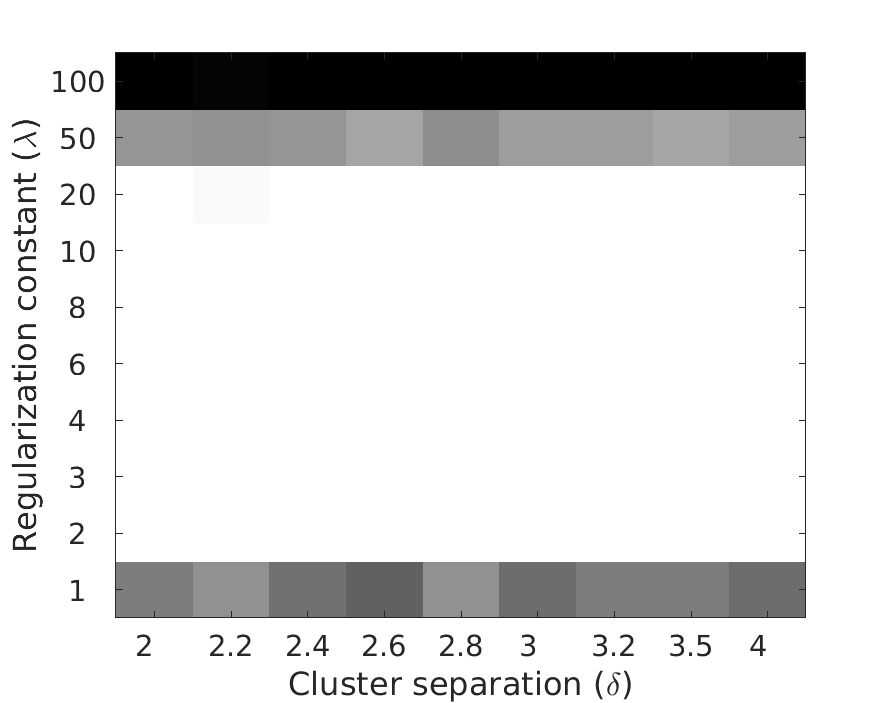
\includegraphics[width=0.45\textwidth]{figures/optimizationClustering/deltaLambda.png}
  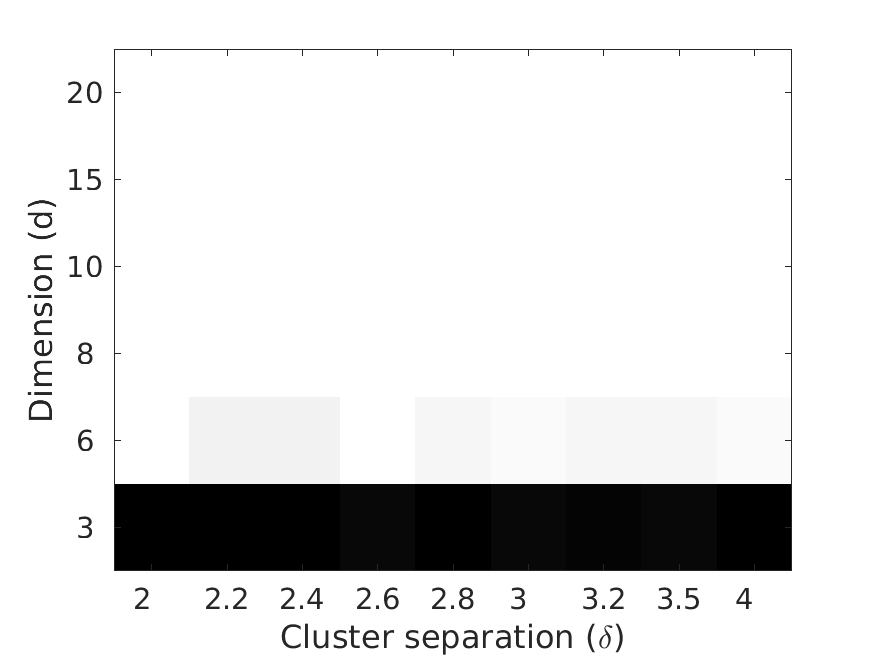
\includegraphics[width=0.45\textwidth]{figures/optimizationClustering/deltaD.png}
  \caption{Heatmap showing the probability of success of the $k$-means regularised sdp algorithm. Lighter color indicates probability closer to one while darker indicates probability closer to zero.}
\end{figure}
\begin{figure}
  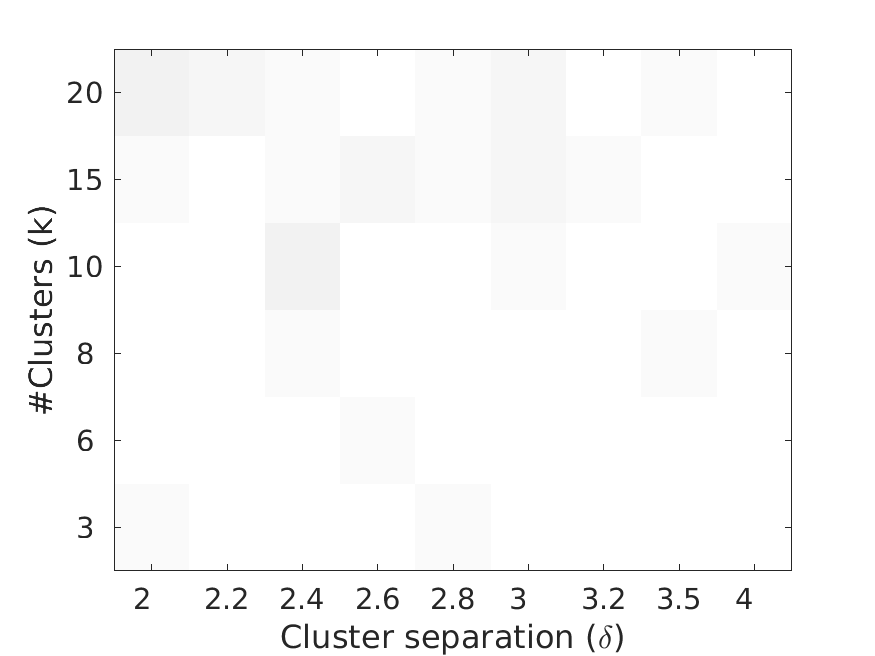
\includegraphics[width=0.45\textwidth]{figures/optimizationClustering/deltaK.png}
  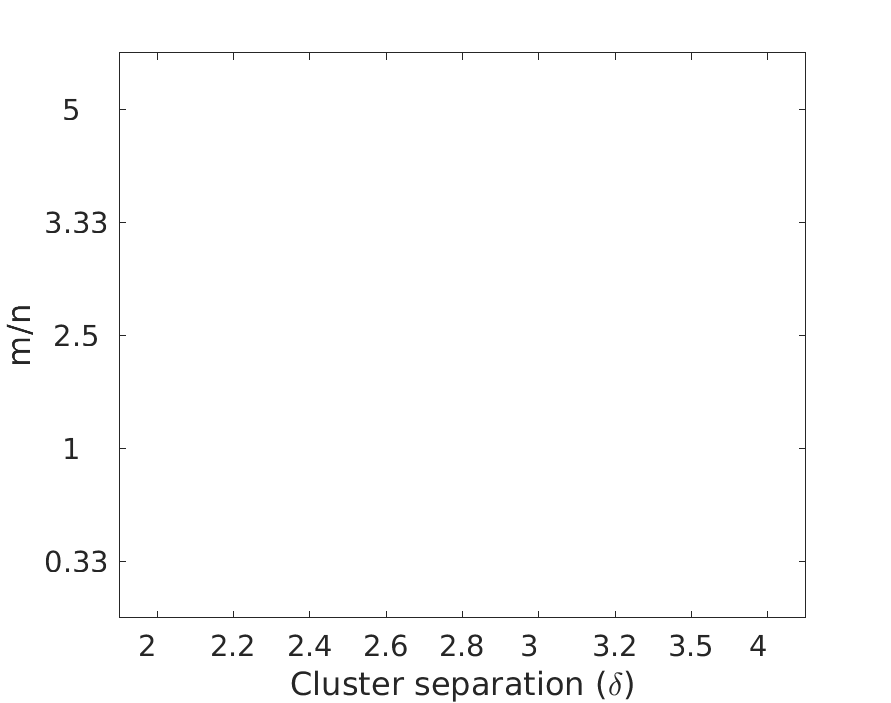
\includegraphics[width=0.45\textwidth]{figures/optimizationClustering/deltaM.png}
  \caption{Heatmap showing the probability of success of the $k$-means regularised sdp algorithm. Lighter color indicates probability closer to one while darker indicates probability closer to zero.$m$ denotes the number of noisy points while $n$ denotes the number of points in the smallest cluster.}
\end{figure}
\begin{figure}
  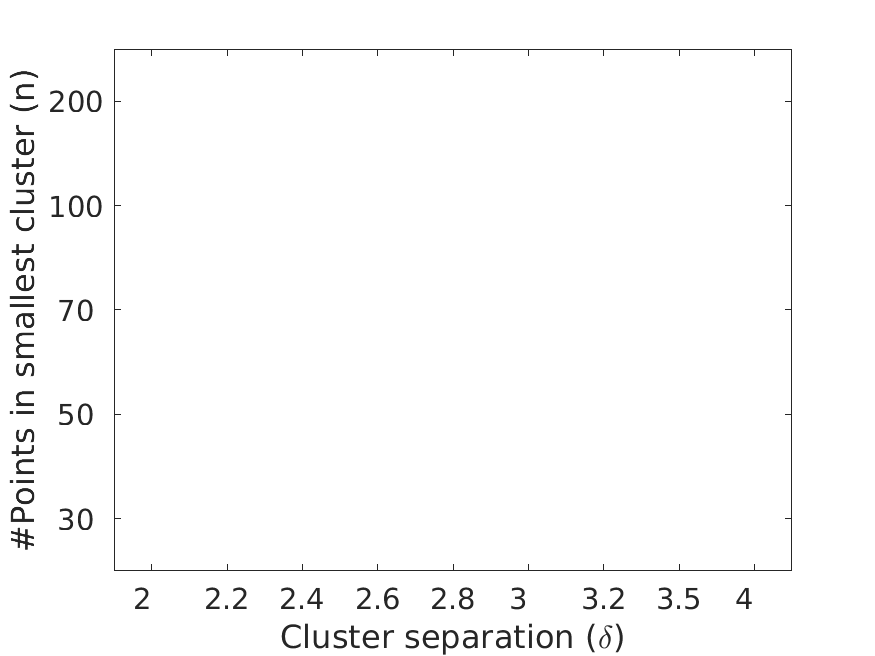
\includegraphics[width=0.45\textwidth]{figures/optimizationClustering/deltan.png}
  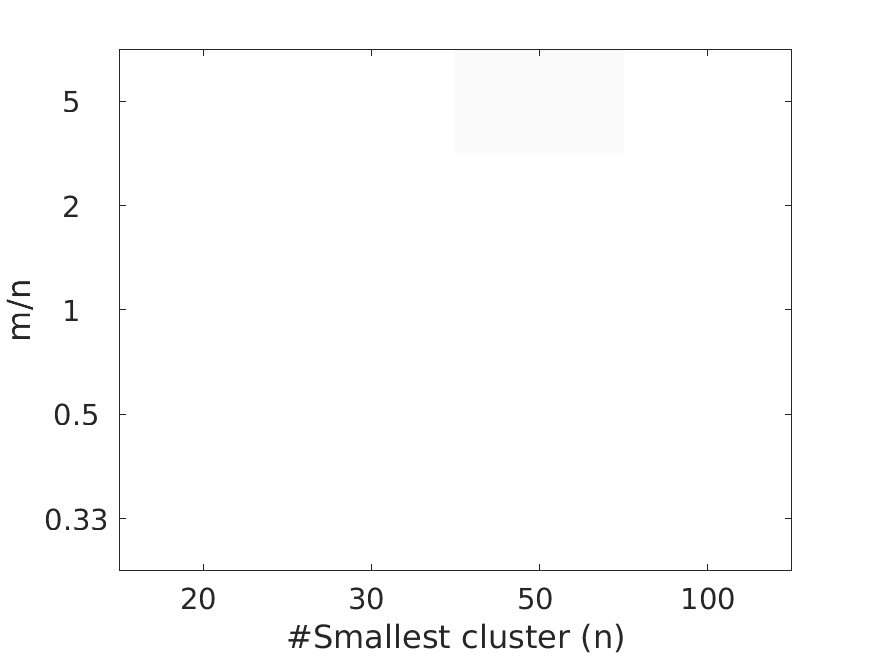
\includegraphics[width=0.45\textwidth]{figures/optimizationClustering/nM.png}
  \caption{Heatmap showing the probability of success of the $k$-means regularised sdp algorithm. Lighter color indicates probability closer to one while darker indicates probability closer to zero. $m$ denotes the number of noisy points while $n$ denotes the number of points in the smallest cluster.}  
\end{figure}

\section{Technical lemma}
\begin{theorem}[Thm. 5.41 in \cite{vershynin2010introduction}]
\label{a-thm:spectralNormCOncentration}
Let $A$ be an $N\times d$ matrix whose rows $A_i$ are independent isotropic random vectors in $\mb R^d$. Let $m$ be a number such that $\|A_i\| \le \sqrt{m}$ almost surely for all $i$. Then for every $t$, one has
$$\sqrt{N} - t\sqrt{m} \le \sigma_{\min}(A) \le \sigma_{\max}(A) \le \sqrt{N} + t\sqrt{m}$$
with probability atleast $1-2d\exp(-ct^2)$, where $c$ is an absolute constant. $\sigma_{\min}$ and $\sigma_{\max}$ are the spectral norms or the minimum and maximum eigenvalues respectively of the matrix $A$.
\end{theorem}

\end{subappendices}

\chapter{Finding cluster structure amidst background noise}
\label{chapter:clusteringNoise}
\ifdefined\COMPLETE
\else
\documentclass[12pt]{article}
%\usepackage{llncsdoc}
%\usepackage[boxruled]{algorithm2e}

\usepackage[boxruled]{algorithm2e}
\usepackage{amsmath,amssymb,amstext,amsthm}

\usepackage{graphicx}
\usepackage{hyperref}
\usepackage[toc,page]{appendix}

\usepackage{enumitem}
\usepackage{tikz}
\usetikzlibrary{shapes, calc, arrows, through, intersections, decorations.pathreplacing, patterns}

\newtheorem{theorem}{Theorem}
\newtheorem{fact}[theorem]{Fact}
\newtheorem{definition}[theorem]{Definition}
\newtheorem{conj}[theorem]{Conjecture}
\newtheorem{smallLemma}{Claim}

\newcommand{\mc}{\mathcal}
\newcommand{\mb}{\mathbf}
\DeclareMathOperator*{\argmin}{arg\,min}
\DeclareMathOperator*{\argmax}{arg\,max}
\DeclareMathOperator{\vcdim}{VC-Dim}
\DeclareMathOperator{\vol}{vol}

\renewcommand\labelitemi{$\bullet$}

\makeatletter  %% this is crucial
\renewcommand\subsubsection{\@startsection{subsubsection}{3}{\z@}%
   {-18\p@ \@plus -4\p@ \@minus -4\p@}%
   {8\p@ \@plus 4\p@ \@minus 4\p@}%     <-- this
   {\normalfont\normalsize\bfseries\boldmath
   \rightskip=\z@ \@plus 8em \pretolerance=10000}}
\makeatother   %% this is crucial
\setcounter{secnumdepth}{3}

\makeatletter
\renewcommand{\algocf@caption@boxruled}{%
  \hrule
  \hbox to \hsize{%
    \vrule\hskip-0.4pt
    \vbox{
       \vskip\interspacetitleboxruled%
       \unhbox\algocf@capbox\hfill
       \vskip\interspacetitleboxruled
       }%
     \hskip-0.4pt\vrule%
   }\nointerlineskip%
}%
\makeatother


\begin{document}
\fi

Clustering is an umbrella term for a wide variety of unsupervised data processing techniques. A relatively comprehensive description of clustering is  that it aims to group together data instances that are similar, while separating dissimilar objects. Most of the common clustering tools output a partitioning of the input data into groups, clusters, that share some form of cohesiveness or between-cluster separation requirement\footnote{The assignment to clusters can sometimes be probabilistic, and clusters may be allowed to intersect, but these aspects are orthogonal to the discussion in this chapter.}. However, in many cases, real data sets, in particular large ones, have on top of such cohesive separated groups, a significant amount of ``background" unstructured data. An obvious example of such a scenario is when the input data set is the set of pixels of an image and the goal of the clustering is to detect groups of pixels that correspond to objects in that image. Clustering in such situations is the focus of this work. Maybe surprisingly, this topic has received relatively little attention in the clustering research community, and even less so when it comes to theoretical work. 

The discussion of finding clustering structure in data sets that also contain subsets that do not conform well to that structure usually falls under the terminology of noise robustness (see e.g., \cite{balcan2012clustering},\cite{ackerman2009clusterability},\cite{dave1993robust}, \cite{cuesta1997trimmed},\cite{garcia2008general}). However, noise robustness, at least in that context, addresses the noisy part of the data as either generated by some specific generative model (like uniform random noise, or Gaussian perturbations) or refers to worst-case adversarially generated noisy data. In this chapter we take a different approach. What distinguishes the noise that we consider form the ``clean" part of the input data is that it is \emph{structureless}. The exact meaning of such a notion of structurlessness may vary depending on the type of structure the clustering algorithm is aiming to detect in the data. We focus on defining structurelessness as  not having significantly large dense subsets. We believe that such a notion is well suited to address ``gray background" contrasting with cohesive subsets of the data that are the objects that the clustering aims to detect. 

The distinction between structured and unstructured parts of the data requires, of course, a clear notion of relevant structure. For that, we resort to a relatively large body of recent work proposing notions of clusterable data sets. That work was developed mainly to address the gap between the computational hardness of (the optimization problem of) many common clustering objectives and the apparent feasibility of clustering in practical applications. We refer the reader to \cite{ben2015computational} for a survey of that body of work. Here, we focus on two such notions, one based on the $\alpha$-center-proximity introduced by \cite{awasthi2012center} and the other, $\lambda$-separation, introduced by \cite{ben2014clustering}.

Our approach diverges from previous discussions of clusterable inputs in yet another aspect. Much of the theoretical research of clustering algorithms views clustering as an optimization problem. For some predetermined objective function (or clustering cost), the algorithm's task is to find the data partitioning that minimizes that objective. In particular, this approach is shared by all the works surveyed in \cite{ben2015computational}. However, in many practical situations the reality is different. Given a large data set to cluster, often-times there is no way a user may know what is the cost of the optimal clustering of that data, or how close to optimal the algorithm's outcome is. Instead, a user might have a notion of meaningful cluster structure, and will be happy with any outcome that meets such a requirement. Consequently, our algorithms aim to provide meaningful clustering solutions (where ``meaningful" is defined in a way inspired by the above mentioned notions of clusterability) without reference to any particular optimization objective function. Our algorithms efficiently compute a hierarchical clustering tree that captures all such meaningful solutions. One should notice that all of those notions of clusterability (those under which it can be show that an objective-minimizing clustering can be found efficiently) assume that there exists an optimal solution that satisfies the meaningfulness condition (such as being perturbation robust, or having significantly smaller distances of points to their own cluster centers than to other centers). Under those assumptions, an algorithm that outputs a tree capturing all meaningful solutions, allows efficient detection of the cost-optimal clustering (in fact, the algorithms of \cite{balcan2012clustering} also yield such trees, for clean, noiseless inputs). Consequently, under the assumptions of those previous works, our algorithms yield an efficient procedure for finding such an optimal solution.

\section{Related Work}
The goal of clustering is to partition a set of objects into {\em dissimilar} subsets of {\em similar} objects. Based on the definition of similarity, the optimal solution to a clustering task is achieved by optimizing an objective function. Although solving this optimization problem is usually NP-hard, the clustering task is routinely and successfully employed in practice. This gap between theory and practice recommends characterizing the real world data sets by defining mathematical notions of {\em clusterable} data. As a result, provably efficient clustering algorithms can be found for these so called {\em nice} data.  

In the past few years, there has been a line of work on defining notions of clusterability. The goal of all these methods has been to show that clustering is computationally efficient if the input $X$ enjoys some nice structure. In \cite{bilu2012stable}, a clustering instance is considered to be \emph{stable} if the optimal solution to a given objective function does not change under small multiplicative perturbations of distances between the points. Using this assumption, they give an efficient algorithm to find the max-cut clustering of graphs which are resilient to $O(\sqrt{|X|})$ perturbations. Using a similar assumption, \cite{ackerman2009clusterability} considered additive perturbations of the underlying metric and designed an efficient algorithm that outputs a clustering with near-optimal cost. 

In terms of clusterability conditions, the most relevant previous papers are those addressing clsutering under {\em $\alpha$-center proximity} condition (see Def.~\ref{defn:alphacp}).
Assuming that the centers belong to $X$ ({\em proper} setting),  \cite{awasthi2012center} shows an efficient algorithm that outputs the optimal solution of a given center-based objective assuming that optimal solution satisfies the $(\alpha > 3)$-center proximity. This result was improved to $(\alpha = \sqrt{2} + 1 \approx 2.4)$ when the objective is $k$-median \cite{balcan2012clustering}. In \cite{ben2014data} it was shown that unless P$=$NP such a result cannot be obtained for $(\alpha <2)$-center proximal inputs.

However, as mentioned above, these results apply only to the noiseless case.
Few methods have been suggested for analyzing clusterability in the presence of noise. 
\cite{balcan2012clustering} considers a dataset which has $\alpha$-center proximity except for an $\epsilon$ fraction of the points. They give an efficient algorithm which provides a $1+O(\epsilon)$-approximation to the cost of the $k$-median optimal solution when $\alpha > 2+\sqrt{7} \approx 4.6$. Note that, while this result applies to adversarial noise as well, it only yields an approximation to the desired solution and  the approximation guarantee is heavily influenced by the size of noise. 

In a different line of work, \cite{ben2014clustering} studied the problem of robustifying any center-based clustering objective to noise. To achieve this goal, they introduce the notion of {\em center separation} (look at Def. \ref{defn:lambdacs}). Informally, an input has center separation when it can be covered by $k$ well-separated set of balls.
Given such an input, they propose a paradigm which converts any center-based clustering algorithm into a clustering algorithm which is robust to small amount of noise.
Although this framework works for any objective-based clustering algorithm, it requires a strong restriction on the noise and clusterability of the data. For example, when the size of the noise is $\frac{5}{100}|X|$, their algorithm is able to obtain a robustified version of $2$-median, only if $X$ is covered by $k$ unit balls which are separated with distance $10$. 

In this work, we consider a natural relaxation of \cite{balcan2012clustering,ben2014clustering}, with the goal to capture more realistic domains containing arbitrary amount of noise, assuming that noise is \emph{structureless} (in a precise sense defined below). For example, in \cite{balcan2012clustering}, the size of the noise $|\mc N| \le \frac{m(C)}{8}$ (where $m(C)$ is size of the smallest cluster). Our algorithms can handle much larger amount of noise as long as they satisfy the {\it structureless} condition.

We define a novel notion of ``gray background" noise. Informally, we call noise {\em structureless} if it does not have similar structure to a {\em nice} cluster at any part of the domain. Under that definition (look at Def.~\ref{def:alphaeta}), our positive, efficient clustering results, do not depend on any restriction on the size of the noise. 

Given a clusterable input $X$ which contains {\em structureless} noise, we propose an efficient algorithm that outputs a hierarchical clustering tree of $X$ that captures all {\em nice} clusterings of $X$. Our algorithm perfectly recovers the underlying {\em nice} clusterings of the input and its performance is independent of number of noisy points in the domain. 

We complement our algorithmic results by proving that under more relaxed conditions, either on the level of clusterability of the clean part of the data, or on the unstructuredness requirements on the noise, such results become impossible. 

%%%%%%%%%%%%%%%%%%%%%%%%%%%%%%%%%%%%%%%%%%%%%%%%%%%%%%%%%%%%%%%%%%%%%%%%%%%%%%%%%%

\subsection{Outline}
The rest of this chapter is structured as follows. In Section \ref{sec:Notation}, we present our notation and formal definitions. In Section \ref{Noise_justify} we show that the type of noise that we address in this paper is likely to arise under some natural assumptions on the data generating process. In Section \ref{section:cp}, we present an efficient algorithm that, for any input set $X$ which contains structureless noise, recovers all the underlying clusterings of non-noise subset of $X$ that satisfies $\alpha$-center proximity for $\alpha > 2+\sqrt{7}$. We complement these results by proving that for $\alpha \leq 2\sqrt{2}+3$ in the case that we have arbitrary noise and for $\alpha \leq \sqrt{2}+3$ in the case of structureless noise, efficient discovery of all nicely structured subsets is not possible.

In Section~\ref{sec:cswithout}, we describe an efficient algorithm that, for any input $X$, recovers all the underlying clusterings of $X$ that satisfy $\lambda$-center separation for $\lambda \geq 3$. We also prove that it is NP-Hard to improve this to $\lambda \leq 2$. In Section~\ref{sec:cswith}, we consider a similar problem in the presence of either arbitrary or structureless noise. We propose an efficient algorithm that, for any input $X$ which contains structureless noise, recovers all the underlying clusterings of non-noise subset of $X$ that satisfy $\lambda$-center separation for $\lambda \geq 4$. We will also show that this result is tight for the case of structureless noise. We complement our results by showing that, under arbitrary noise assumption, no similar positive result can be achieved for $\lambda \leq 6$. Note that all our missing proofs can be found in the appendix.

\section{Notation and definition}
\label{sec:Notation}
Let $(\mb M, d)$ be a metric space. Given a data set $X \subseteq \bf M$ and an integer $k$. A $k$-clustering of $X$ denoted by $\mc C_{X}$ is a partition of $X$ into $k$ disjoints sets. Given points $c_1, \ldots, c_k \in \mb M$, we define the clustering induced by these points (or {\it centers}) by assigning each $x \in X$ to its nearest center. In the {\it steiner} setting, the centers can be arbitrary points of the metric space $\mb M$. In the {\it proper} setting, we restrict our centers to be members of the data set $X$. In this paper, we will be working in the {\bf proper} setting.

For any set $\mc A\subseteq X$ with center $c\in \mb M$, we define the radius of $\mc A$ as $r_c(\mc A) = \max_{x \in \mc A} d(x, c)$. Throughout the paper, we will use the notation $\mc C_{X}$ to denote the clustering of the set $X$ and $\mc C_{S}$ to denote the clustering of some $S\subseteq X$. 

\begin{definition}[$r(\mc C_{X})$ , $m(\mc C_{X})$] Given a clustering $\mc C_{X} = \{C_1, \ldots, C_k\}$ induced by centers $c_1, \ldots, c_k \in \mb M$, we define $m(\mc{C}_{\mc{X}}) = \min_i |C_i|$ and $r(\mc{C}_{\mc{X}}) = \max_i \thinspace r(C_i)$.
\end{definition}

\begin{definition}[$\mc C_{X}$ restricted to a set] Given $S \subseteq X$ and a clustering $\mc C_{X} = \{C_1, \ldots, C_k\}$ of the set $X$. We define $\mc C_{X}$ restricted to the set $S$ as $\mc C_{{X}|_{S}} = \{C_1 \cap S, \ldots, C_k \cap S\}$. 
\end{definition}

\begin{definition}[$\mc C_{X}$ respects $\mc C_{S}$] Given $S \subseteq X$, clusterings $\mc C_{X} = \{C_1, \ldots, C_k\}$ and $\mc C_{S} = \{S_1, \ldots, S_{k'}\}$. We say that $\mc C_{X}$ respects $\mc C_{S}$ if $\mc C_{{X}|_{S}} = \mc C_{S}$.
\end{definition}

\begin{definition}[$\mc T$ or $\mc L$ captures $\mc C_{S}$]Given a hierarchical clustering tree $\mc T$ of $X$ and a clustering $\mc C_{S}$ of $S \subseteq X$.  We say that $\mc T$ captures $\mc C_{S}$ if there exists a pruning $\mc P$ which respects $\mc C_{S}$. 

Similarly, given a list of clusterings $\mc L$ of $X$ and a clustering $\mc C_{S}$ of $S \subseteq X$. We say that $\mc L$ captures $\mc C_{S}$ if there exists a clustering $\mc C_{X} \in \mc L$ which respects $\mc C_{S}$. 
\end{definition}

\begin{definition}[$\alpha$-center proximity \cite{awasthi2012center}]
\label{defn:alphacp}
A clustering $\mc C_{X} = \{C_1, \ldots, C_k\}$ satisfies $\alpha$-center proximity w.r.t $X$ and $k$ if there exist centers $c_1, \ldots, c_k \in \mb M$  such that the following holds. For all $x \in C_i$ and $i\neq j$, $\alpha d(x, c_i) < d(x, c_j)$
\end{definition}

Next, we formally define our notion of structureless noise. Roughly, such noise should be scattered sparsely, namely, there should be no significant amount of noise in any small enough ball. Note that such a restriction does not impose any upper bound on the number of noise points.

\begin{definition}[$(\alpha, \eta)$-center proximity]
\label{def:alphaeta}
Given $S \subseteq X$, a clustering $\mc C_{S} = \{S_1, \ldots, S_k\}$ has $(\alpha, \eta)$-center proximity w.r.t $X, S$ and $k$ if there exists centers $s_1, \ldots, s_k \in \mb M$  such that the following holds.
\begin{itemize}[nolistsep, noitemsep]
\label{defn:alphacpnoise}	

\item[$\diamond$] {\bf $\alpha$-center proximity}: For all $x \in S_i$ and $i\neq j$, $\thinspace\alpha d(x, s_i) < d(x, s_j)$
\item[$\diamond$]{\bf $\eta$-sparse noise}: For any ball $B$, $r(B)\leq \eta \thinspace r(\mc{C}_{S}) \implies |B\cap (X\setminus S)| < \frac{m(\mc C_{S})}{2}$
\end{itemize}
%Note: In this paper, we will restrict the centers $s_i \in X$ (proper setting). 
\end{definition}

\begin{definition}[$\lambda$-center separation \cite{ben2014clustering}]
\label{defn:lambdacs}
A clustering $\mc C_{X} = \{C_1, \ldots, C_k\}$ has $\lambda$-center separation w.r.t $X$ and $k$ if there exists centers $c_1, \ldots, c_k \in \mb M$ such that $\mc C_{X}$ is the clustering induced by these centers and the following holds. For all $i\neq j$, $d(c_i, c_j) > \lambda r(\mc{C}_{\mc{X}})$
\end{definition}

\begin{definition}[$(\lambda, \eta)$-center separation]
Given $S \subseteq X$, a clustering $\mc C_{S}$ has $(\lambda, \eta)$-center separation w.r.t $X, S$ and $k$ if there exists centers $s_1, \ldots, s_k \in \mb M$ such that $\mc C_{X}$ is the clustering induced by these centers and the following holds.

\begin{itemize}[nolistsep, noitemsep]
\label{defn:lambdacsnoise}	

\item[$\diamond$] {\bf $\lambda$-center separation}: For all $i\neq j$, $\thinspace d(s_i, s_j) > \lambda r({\mc C}_{S})$
\item[$\diamond$]{\bf $\eta$-sparse noise}: For any ball $B$, $r(B)\leq \eta \thinspace r(\mc{C}_{S}) \implies |B\cap (X\setminus S)| < \frac{m(\mc C_{S})}{2}$
\end{itemize}
%Note: In the setting of this paper, we will restrict the centers $s_i \in X$. 
\end{definition}

We denote a ball of radius $x$ at center $c$ by $B(c, x)$. We denote by $P_{i}(c)$ a collection of $i$ many points sitting on the same location $c$. If the location is clear from the context, we will use the notation $P_i$.

%\noindent{\textbf{Important Note}}: For the sake of generality, all the definitions of this section has been stated in the steiner setting. It is important to note that, in this paper, we will only use these definitions in the {\bf proper} setting.
%%%%%%%%%%%%%%%%%%%%%%%%%%%%%%%%%%%%%%%%%%%%%%%%%%%%%%%%%%%%%%%%%%%%%%%%%%%%%%%%%%%%%%%%%%%%%%%%%%%%%%%%%%%%%%%%%%%%%%%%%%%%%%%%%%%%%%%%%%%%%%%%%%%%%%%%%%%%%%%%


\section{Justification of sparse noise}
\label{Noise_justify}
In this section, we examine our sparseness condition. We will show that if the set of points $\mc N$ are generated by a non concentrated distribution in a ball in $\mb R^d$ then with high probability, as long as $\mc N$ is not too large (so as to``
drown" the original data set), it will satisfy the sparse noise condition. The proof is based on the epsilon approximation theorem for classes of finite VC-dimension, applied to the set of balls in $\mb R^d$. The following, rather natural, definition of non concentrated distribution was introduced in \cite{balcan2012distributed}.
\begin{definition} 
A probability distribution over the $d$-dimensional unit ball is \emph{non-concentrated} if, for some constant $c$, the probability density of any point $x$ is at most $c$ times its density under the uniform distribution over that ball.
\end{definition}

\begin{theorem}[Noise by non concentrated distribution is sparse]
\label{theorem:sparse}
Let $X$ be a ball of radius $R$ in $\mb R^d$ and $S \subseteq X$. Let $\mc C$ be a clustering of $S$ which satisfies $\alpha$-center proximity (or $\lambda$-center separation). Given parameters $\epsilon, \delta \in (0,1)$. Let $\mc N \subseteq X$ be picked i.i.d according to a non concentrated probability distribution. If $|\mc N| < c  \left( \frac{R}{r(C) \eta} \right) ^d m(C)$
then with high probability, $S \cup \mc N$  satisfies $(\alpha, \eta)$-center proximity (the $(\lambda, \eta)$-center separation, respectively).
\end{theorem}
\begin{proof}
Let $H = \{B \text{ is a ball }: B \subseteq X\}$. Observe that $\vcdim(H) = d+1$. Let $\gamma := \frac{r(C)}{R}$. Since the noise-generating distribution $P$ is $c$-concentrarted, for every ball $B$, $P(B) \leq c \frac{\vol(B)}{\vol(X)} = c\gamma^d$. Now, the fundamental $\epsilon$-approximation theorem (Theorem~\ref{theorem:vceapprox}) establishes the result.
\qed
\end{proof}

\noindent Note that Theorem~\ref{theorem:sparse} shows that the cardinality of the noise set, $|\mc N|$, can be much bigger than the size of the smallest cluster $m(\mc C)$. 

\section{Center Proximity}
\label{section:cp}

In this section, we study the problem of recovering $(\alpha, \eta)$-center proximal clusterings of a set $X$, in the presence of noise. The goal of our algorithm is to produce an efficient representation (hierarchical clustering tree) of all possible $(\alpha, \eta)$-center proximal nice clusterings rather than to output a single clustering or to optimize an objective function. Here is a more precise overview of the results of this section: 
\begin{itemize}[nolistsep,noitemsep,leftmargin=*]
\item  {\it Positive result under sparse noise} - In Section \ref{section:positiveResultSparseNoise}, we give our main result under sparse noise. If $\alpha \ge 2 + \sqrt{7} \approx 4.6$ and $\eta \ge 1$; for any value of $t$, Alg.~\ref{alg:alphacp} outputs a tree which captures all clusterings $\mc C^*$ (of a subset of $X$) which satisfy $(\alpha, \eta)$-center proximity and $m(C^*)=t$.
\item  {\it Lower bound under sparse noise} - In Section \ref{section:alphaLowerBoundSparse}, we show that if $\alpha \le 2 + \sqrt{3} \approx 3.7$ and $\eta \le 1$ then there is no tree and no list of `small' size ($< 2^{k/2}$) which can capture all clusterings $\mc C$ (of a subset of $X$) which satisfy $(\alpha, \eta)$-center proximity even for a fixed value of the size of the smallest cluster $(m(C) = t)$.
\item {\it Lower bound with arbitrary noise} - In Section \ref{section:alphaLowerBoundArbitrary}, we show that for a given value of a parameter $t$, if $\alpha \le 2\sqrt{2} + 3 \approx 5.8$ and the number of noisy points exceeds $\frac{3}{2}t$ then no tree can capture all clusterings $\mc C$ (of a subset of $X$) which satisfy $\alpha$-center proximity even for fixed $m(\mc C) = t$. Identical result holds for `small' ($<2^{k/2}$) lists if the number of noisy points exceeds $\frac{3k}{2}t$.
\end{itemize} 

\subsection{Positive result under sparse noise}
\label{section:positiveResultSparseNoise}
Given a clustering instance $(X, d)$ and a parameter $t$, we introduce an efficient algorithm which outputs a hierarchical clustering tree $\mc T$ of $X$ with the following property. For every $k$, for every $S \subseteq X$ and for every $k$-clustering $\mc C_{S}$ which satisfies $(\alpha, \eta)$-center proximity (for $\alpha \ge 2 + \sqrt{7}$ and $ \eta \ge 1)$ and $m(\mc C_{S}) = t$, $\mc T$ captures $\mc C_{S}$. It is important to note that our algorithm only knows $X$ and has no knowledge of the set $S$.

Our algorithm has a linkage based structure similar to \cite{balcan2012clustering}. However, our method benefits from a novel {\it sparse distance condition}. We introduce the algorithm in Alg.~\ref{alg:alphacp} and prove its efficiency and correctness in Theorem~\ref{thm:algcptime} and Theorem~\ref{thm:alphacpnoise} respectively. 

\begin{definition}[Sparse distance condition]
	 Given a clustering $\mc C = \{C_1,\\\ldots,C_k\}$ of the set $X$ and a parameter $t$. We say that the ball $B \subseteq X$ satisfies the sparse distance condition w.r.t clustering $\mc C$ when the following holds.
\begin{itemize}[noitemsep,nolistsep,leftmargin=*]
\item $|B| \ge t$.
\item For any $C_i \in \mc C$, if $C_i \cap B \neq \emptyset$, then $C_i \subseteq B$ or $|B \cap C_i| \ge t/2$.
\end{itemize}
\end{definition}

Intuitively, Alg.~\ref{alg:alphacp} works as follows. It maintains a clustering $\mc C^{(l)}$, which is initialized so that each point is in its own cluster. It then goes over all pairs of points $p, q$ in increasing order of their distance $d(p, q)$. If $B(p, d(p,q))$ satisfies the sparse distance condition w.r.t $\mc C^{(l)}$, then it merges all the clusters which intersect with this ball into a single cluster and updates $\mc C^{(l)}$. Furthermore, the algorithm builds a tree with the nodes corresponding to the merges performed so far. We will show that for all $S \subseteq X$ which are $(\alpha, \eta)$-proximal $t$-min nice and for all clusterings $\mc C_S$ which have $(\alpha, \eta)$-center proximity, Alg.~\ref{alg:alphacp} outputs a tree which captures $\mc C_S$.

\RestyleAlgo{ruled}
\SetAlgoNoLine
\LinesNumbered
\SetNlSkip{-0.4em}

\begin{algorithm}
\Indp\KwIn{$(X, d)$ and $t$}
\KwOut{A hierarchical clustering tree $T$ of $X$.}
	
\vspace{0.1in} Let $\mc C^{(l)}$ denote the clustering $X$ after $l$ merge steps have been performed. Initialize $\mc C^{(0)}$ so that all points are in their own cluster. That is, $\mc C^{(0)} = \{ \{x\}: x \in X\}$.
	
	Go over all pairs of points $p, q$ in increasing order of the distance $d(p, q)$. If $B = B(p, d(p, q))$ satisfies the sparse distance condition then\\
	Merge all the clusters which intersect with $B$ into a single cluster.
	
	\vspace{0.1in}Output clustering tree $T$. The leaves of $T$ are the points in dataset $X$. The internal nodes correspond to the merges performed.
\caption{Alg. for $(\alpha, \eta)$-center proximity with parameter $t$}	
\label{alg:alphacp}
\end{algorithm}
\vspace{-.1in}
\begin{theorem}
\label{thm:alphacpnoise}
Given a clustering instance $(X, d)$ and a parameter $t$. Alg.~\ref{alg:alphacp} outputs a tree $\mc T$ with the following property. For all $k$, $S \subseteq X$ and for all $k$-clusterings $\mc C^*_{S} = \{S_1^*, \ldots, S_k^*\}$ which satisfy $(2+\sqrt{7}, 1)$-center proximity the following holds. If $m(\mc C_{S}^*) = t$ then $\mc T$ captures $\mc C_{S}$.
\end{theorem}

\begin{theorem}
\label{thm:algcptime}
Given clustering instance $(X, d)$ and $t$. Alg.~\ref{alg:alphacp} runs in  $poly(|X|)$.
\end{theorem}

\begin{proof}
Let $n = |X|$. Checking if $B$ satisfies the sparse-distance condition takes $O(n)$ time and hence the algorithm runs in $O(n^3)$ time.
\end{proof}

\subsection{Lower bound under sparse noise}
\label{section:alphaLowerBoundSparse}
\begin{theorem}
\label{thm:noalgalphacp}
Given the number of clusters $k$ and parameter $t$. For all $\alpha \le 2+\sqrt{3}$ and $\eta \le 1$ there exists a clustering instance $(X, d)$ such that any clustering tree $\mc T$ of $X$ has  the following property. There exists $S \subseteq X$ and clustering $\mc C_{S}$ which satisfies $(\alpha, \eta)$-center proximity and $ m(\mc C_{S}) = t$ but $\mc T$ doesn't capture $\mc C_{S}$.
\end{theorem}

\begin{theorem}
\label{thm:nolistalphacp}
Given the number of clusters $k$ and parameter $t$. For all $\alpha \le 2+\sqrt{3}$, $\eta \le 1$ there exists $(X, d)$ such that any list $\mc L$ (of clusterings of $X$) has  the following property. If $|\mc L| < 2^{\frac{k}{2}}$ then there exists $S \subseteq X$ and clustering $\mc C_{S}$ which satisfies $(\alpha, \eta)$-center proximity and $ m(\mc C_{S}) = t$ but $\mc L$ doesn't capture $\mc C_{S}$.
\end{theorem}

\subsection{Lower bound under arbitrary noise}
\label{section:alphaLowerBoundArbitrary}

\begin{theorem}
\label{thm:nosparsealg}
Given the number of clusters $k$ and a parameter $t$. For all $\alpha < 2\sqrt 2 + 3$ there exists $(X, d)$ such that any clustering tree $\mc T$ of $X$ has the following property. There exists $S \subseteq X$ and there exists clustering $\mc C_{S}$ which satisfies $\alpha$-center proximity such that $m(\mc C_{S}) = t$ and the following holds. If $|X \setminus S| \ge \frac{3m(\mc C_{S})}{2}+5$, then $\mc T$ doesn't capture $\mc C_{S}$.
\end{theorem}

\begin{theorem}
\label{thm:nosparselistalphacp}
Given the number of clusters $k$ and parameter $t$. For all $\alpha \le 2+\sqrt{2}+3$ there exists $(X, d)$ such that any list $\mc L$ (of clusterings of $X$) has  the following property. There exists $S \subseteq X$ and there exists clustering $\mc C_{S}$ which satisfies $\alpha$-center proximity such that $m(\mc C_{S}) = t$ and the following holds. If $|\mc L| < 2^{\frac{k}{2}}$ and $|X \setminus S|\ge \frac{k}{2}(\frac{3m(\mc C_{S})}{2}+5)$, then $\mc L$ doesn't capture $\mc C_{S}$.
\end{theorem}

\section{Center Separation}
\label{sec:cs}
 
\subsection{Center Separation without noise}
\label{sec:cswithout}

In this section, we study the problem of recovering $\lambda$-center separated clusterings of a set $X$, in the absence of noise. We do not want to output a single clustering but to produce an efficient representation (hierarchal clustering tree) of all possible $\lambda$-center separated nice clusterings. In Section \ref{section:positiveNoNoiseLambda} we give an algorithm that generates a tree of all possible $\lambda$-center separated clusterings of $X$ for $\lambda > 3$.  In Section \ref{section:lowerBdNoNoiseLambda}, we prove that for  $\lambda < 2$, it is NP-Hard to find any such clustering.

%%%%%%%%%%%%%%%%%%%%%%%%%%%%%%%%%%%%%%%%%%%%%%%%%%%%%%%%%%%%%%%%%%%%%%%%%%%%%%%%%%

\subsubsection{Positive result under no noise}
\label{section:positiveNoNoiseLambda}
Given a clustering instance $(X, d)$, our goal is to output a hierarchical clustering tree $T$ of $X$ which has the following property. For every $k$ and for every $k$-clustering $\mc C_{X}$ which satisfies $\lambda$-center separation, there exists a pruning $\mc P$ of the tree which equals $\mc C_{X}$. Our algorithm (Alg.~\ref{alg:lambdacsNoNoise}) uses single-linkage to build a hierarchical clustering tree of $X$. We will show that when $\lambda \ge 3$ our algorithm achieves the above mentioned goal. 

\begin{algorithm}[!t]
	\SetAlgoLined
	\Indp\KwIn{$(X, d)$}
	\KwOut{A hierarchical clustering tree $T$ of $X$.}
	
	\vspace{2mm} Initialize the clustering so that each point is in its own cluster.
	
	Run single-linkage till only a single cluster remains. Output clustering tree $T$.

\caption{Alg. for $\lambda$-center separation}
\label{alg:lambdacsNoNoise}
\end{algorithm}
\vspace{-.1in}
\begin{theorem}
\label{thm:lambdaNoNoisePositive}
Given $(X , d)$. For all $\lambda \ge 3$, Alg.~\ref{alg:lambdacsNoNoise} outputs a tree $\mc T$ with the following property. For all $k$ and for all $k$-clusterings $\mc C_{X}^* = \{C_1^*, \ldots, C_k^* \}$ which satisfy $\lambda$-center separation w.r.t $X$ and $k$, the following holds. For every $1 \le i \le k$, there exists a node $N_i$ in the tree $T$ such that $C_i^* = N_i$.
\end{theorem}

%%%%%%%%%%%%%%%%%%%%%%%%%%%%%%%%%%%%%%%%%%%%%%%%%%%%%%%%%%%%%%%%%%%%%%%%%%%%%%%%%%

\subsubsection{Lower bound with no noise}
\label{section:lowerBdNoNoiseLambda}
We will prove that for $\lambda \le 2$, finding any solution for $\lambda$-center separation is NP-Hard. \cite{reyzin2012data} proved that finding any solution for $\alpha$-center proximity is NP-Hard for $\alpha < 2$. Our reduction is same as the reduction used in Theorem~1 in \cite{reyzin2012data} and hence we omit the proof.

\begin{theorem}
\label{thm:lambdaNoNoiseLowerBd}
Given a clustering instance $(X, d)$ and the number of clusters $k$. For $\lambda < 2$, finding a clustering which satisfies $\lambda$-center separation is NP-Hard.
\end{theorem}

\subsection{Center Separation in the presence of noise}
\label{sec:cswith}
In this section, we study the problem of recovering $(\lambda, \eta)$-center separated clusterings of a set $X$, in the presence of noise. Here is a more precise overview of the results of this section:
\begin{itemize}[nolistsep,noitemsep,leftmargin=*]
\item  {\it Positive result under sparse noise} - In Section \ref{section:lambdaPositiveResultSparseNoise}, we show that if $\lambda \ge 4$ and $\eta \ge 1$; for any value of parameters $r$ and $t$, Alg.~\ref{alg:lambdacs} outputs a clustering which respects all clusterings $\mc C^*$ (of a subset of $X$) which satisfies $(\lambda, \eta)$-center proximity and $m(C^*)=t$ and $r(C^*) = r$.
\item  {\it Lower bound under sparse noise} - In Section \ref{section:lambdaLowerBoundSparse}, we show that, if $\lambda < 4$ and $\eta \le 1$ then there is no tree and no list of `small' size ($<2^{k/2}$) which can capture all clusterings $\mc C$ (of subset of $X$) which satisfy $(\lambda, \eta)$-center proximity even for fixed values of the size of the smallest cluster $(m(C) = t)$ and maximum radius ($r(C) = r$).
\item {\it Lower bound with arbitrary noise} - In Section \ref{section:lambdaLowerBoundArbitrary}, we show that for a given value of parameters $r$ and $t$, if $\lambda \le 6$ and the number of noisy points exceeds $\frac{3}{2}t$ then no tree can capture all clusterings $\mc C$ (of a subset of $X$) which satisfy $\lambda$-center separation even for fixed $m(\mc C) = t$ and $r(\mc C) = r$. Identical result holds for `small' ($<2^{k/2}$) lists if the number of noisy points exceeds $\frac{3k}{2}t$.
\end{itemize}

\subsubsection{Positive result under sparse noise}
\label{section:lambdaPositiveResultSparseNoise}
We are given a clustering instance $(X, d)$ and parameters $r$ and $t$. Our goal is to output a clustering $\mc C_{X}$ which has the following property. For every $k$, for every $S \subseteq X$ and for every $k$-clustering $\mc C_{S}$ which satisfies $(\lambda, \eta)$-center separation, the clustering $\mc C_{X}$ restricted to $S$ equals $\mc C_{S}$. 

In the next section, we propose a clustering algorithm (Alg.~\ref{alg:lambdacs}) and prove (Theorem~\ref{thm:lambdacsnoise}) that our algorithm indeed achieves the above mentioned goal (under certain assumptions on the parameters $\lambda$ and $\eta$). It is important to note that our algorithm only knows $X$ and has no knowledge of the set $S$. 

Intuitively, Alg.~\ref{alg:lambdacs} works as follows. In the first phase, it constructs a list of balls which have radius at most $r$ and contain at least $t$ points. It then constructs a graph as follows. Each ball found in the first phase is represented by a vertex. If two balls have a `large' intersection then there is an edge between the corresponding vertices in the graph. We then find the connected components in the graph which correspond to the clustering of the original set $X$. 

\begin{algorithm}[!ht]	
	\Indp\KwIn{$(X, d), t$ and $r$}
	\KwOut{A clustering $\mc C$ of the set $X$.}
	
	\vspace{0.1in}\textbf{Phase 1}\\
	Let $\mc L$ denote the list of balls found so far. Initialize $\mc L$ to be the empty set. $\mc L = \emptyset$.
	
	Go over all pairs of points $p, q \in X$ in increasing order of the distance $d(p, q)$. Let $B := B(p, d(p, q))$. If $|B| \ge t$ and $r(B) \le r$ then
	
	\hspace{0.24in}$\mc L = \mc L \thinspace\cup B$
	
	\vspace{0.1in}Output the list of balls $\mc L = \{B_1, \ldots, B_l\}$ to the second phase of the algorithm.
	
	\vspace{0.1in}\textbf{Phase 2}\\
	Construct a graph $G = (V, E)$ as follows. $V = \{v_1, v_2, \ldots, v_l\}$. If $|B_i \cap B_j| \ge t/2$ then construct an edge between $v_i$ and $v_j$.
	
	Find connected components ($G_1, \ldots, G_{k}$) in the graph $G$. 
	
	Merge all the points in the same connected component together to get a clustering $\mc C = \{C_1, \ldots, C_k\}$ of the set $X$.
	
	Assign $x \in X \setminus \mc \cup_i B_i$ to the closest cluster $C_i$. That is, $i := \argmin\limits_{j\in [k]} \min\limits_{y \in C_j}d(x, y)$. Output $\mc C$. 
\caption{Alg. for $(\lambda, \eta)$-center separation with parameters $t$ and $r$}
\label{alg:lambdacs}
\end{algorithm}
\vspace{-.1in}
\begin{theorem}
\label{thm:lambdacsnoise}
Given a clustering instance $(X, d)$ and parameters $r$ and $t$. For every $k$, for every $S \subseteq X$ and for all $k$-clusterings $\mc C^*_{S} = \{S_1^*, \ldots, S_k^*\}$ which satisfy $(4, 1)$-center separation such that $ m(\mc C_{S}^*) = t$ and $r(\mc C_{S}^*) = r$, the following holds. Alg.~\ref{alg:lambdacs} outputs a clustering $\mc C_{X}$ such that $\mc C_{X}|_{S} = \mc C_{S}^*$.
\end{theorem}

\begin{theorem}
\label{thm:alglambdacstime}
Given $(X, d)$ and parameters $r$ and $t$. Alg.~\ref{alg:lambdacs} runs in $poly(|X|)$.
\end{theorem}

\begin{proof}
Let $n = |X|$. Phase 1 of Alg.~\ref{alg:lambdacs} runs in $O(n^2)$ time. Phase 2 gets a list of size $l$. Constructing $G$ and finding connected components takes $O(l^2)$ time. Hence, the algorithm runs in $O(n^2)$ time.
\end{proof}


\subsubsection{Lower bound under sparse noise}
\label{section:lambdaLowerBoundSparse}
\begin{theorem}
\label{thm:noalglambdacs}
Given the number of clusters $k$ and parameters $r$ and $t$. For all $\lambda < 4$ and $\eta \le 1$, there exists a clustering instance $(X , d)$ such that any clustering tree $\mc T$ of $X$ has the following property. There exists $S \subseteq X$ and a $k$-clustering $\mc C_{S} = \{S_1, \ldots, S_k\}$ which satisfies $(\lambda, \eta)$-center separation such that $m(\mc C_{S}) = t$ and $r(\mc C_{S}) = r$, but $\mc T$ doesn't capture $\mc C_{S}$.
\end{theorem}

\begin{theorem}
\label{thm:nolistlambdacs}
Given the number of clusters $k$ and parameters $r$ and $t$. For all $\lambda \le 4$ and $\eta \le 1$ there exists a clustering instance $(X, d)$ such that any list $\mc L$ (of clusterings of $X$) has  the following property. If $|\mc L| < 2^{\frac{k}{2}}$ then there exists $S \subseteq X$ and clustering $\mc C_{S}$ which satisfies $(\lambda, \eta)$-center separation and $ m(\mc C_{S}) = t$ and $r(\mc C_{S}) = r$, but $\mc L$ doesn't capture $\mc C_{S}$.
\end{theorem}


\subsubsection{Lower bound with arbitrary noise}
\label{section:lambdaLowerBoundArbitrary}

\begin{theorem}
\label{thm:nosparselambdaalg}
Given the number of clusters $k$ and parameters $r$ and $t$. For all $\lambda < 6$, there exists a clustering instance $(X , d)$ such that any clustering tree $\mc T$ of $X$ has the following property. There exists $S \subseteq X$ and there exists $k$-clustering $\mc C_{S}$ which satisfies $\lambda$-center separation such that $m(\mc C_{S}) = t$, $r(\mc C_{S}) = r$ and the following holds. If $|X\setminus S|\ge \frac{3t}{2}+5$, then $\mc T$ doesn't capture $\mc C_{S}$ .
\end{theorem}

\begin{theorem}
\label{thm:nosparselistlambdacs}
Given the number of clusters $k$ and parameters $r$ and $t$. For all $\lambda \le 6$ there exists $(X, d)$ such that any list $\mc L$ (of clusterings of $X$) has the following property. There exists $S \subseteq X$ and there exists clustering $\mc C_{S}$ which satisfies $\lambda$-center separation such that $m(\mc C_{S}) = t$, $r(\mc C_{S}) = r$ and the following holds. If $|\mc L| < 2^{\frac{k}{2}}$ and $|X \setminus S|\ge \frac{k}{2}(\frac{3m(\mc C_{S})}{2}+5)$, then $\mc L$ doesn't capture $\mc C_{S}$.
\end{theorem}

\ifdefined\COMPLETE
\else
\end{document}
\fi
\begin{subappendices}
\section{Proofs of missing lemmas and theorems}
\textbf{Proof of Theorem~\ref{thm:alphacpnoise}}
Fix any $\mc S \subseteq \mc X$. Let $\mc C^*_S = \{S_1^*, \ldots, S_k^*\}$ be a clustering of $\mc S$ such that $m(\mc C_{\mc S}^*) = t$ and $\mc C^*_S$ has $(\alpha, \eta)$-center proximity. Denote by $r_i := r(S_i^*)$ and $r = \max r_i$. Define $Y_B^{\mc C} := \{C_i \in \mc C : C_i \subseteq B \text{ or } |B \cap C_i| \ge t/2\}$. Note that whenever a ball $B$ satisfies the sparse-distance condition, all the clusters in $Y_{B}^{{\mc C}^{(l)}}$ are merged together and the clustering $\mc C^{(l+1)}$ is updated. We will prove the theorem by proving two key facts.

\begin{enumerate}[nolistsep, noitemsep, label=\textbf{F.\arabic*},leftmargin=0.3in]
\renewcommand\labelitemi{$\diamond$}
\item \label{fact:1} If the algorithm merges points from a good cluster $S_i^*$ with points from some other good cluster,  then at this step the distance being considered $d = d(p,q) > r_i$.	
\item \label{fact:2} When the algorithm considers the distance $d = r_i$, it merges all points from $S_i^*$ (and possibly points from $\mc X\setminus \mc S$) into a single cluster $C_i$. Hence, there exists a node in the tree $N_i$ which contains all the points from $S_i^*$ and no points from any other good cluster $S_j^*$. 	
\end{enumerate}
Note that the theorem follows from these two facts. Similar reasoning was also used in proof of Lemma 3 in \cite{balcan2012clustering}. We now prove both of these facts formally. 

\noindent\textit{\underline{Proof of Fact.~\ref{fact:1}}}
Let $\mc C^{(l)} = \{C_1, \ldots, C_{k'}\}$ be the current clustering of $\mc X$. Let $l+1$ be the first merge step which merges points from the good cluster $S_i^*$ with points from some other good cluster. Let $p, q \in \mc X$ be the pair of points being considered at this step and $B = B(p, d(p, q))$ the ball that satisfies the sparse distance condition at this merge step. Denote by $Y = Y_{B}^{C^{(l)}}$. We need to show that $d(p, q) > r_i$. To prove this, we need Claim~\ref{claim:fromBothCluster} below. 

\begin{smallLemma}
\label{claim:fromBothCluster}
Let $p, q \in \mc X$ and $B$, $Y$, $S_i^*$ and $C^{(l)}$ be as defined above. If $d(p, q) \le r,$ then $B \cap S_i^* \neq \emptyset$ and there exists $n \neq i$ such that $B \cap S_n^* \neq \emptyset$.
\end{smallLemma}
\vspace{-0.1in} $l+1$ is the first step which merges points from $S_i^*$ with some other good cluster. Hence, $\exists C_i \in Y$ such that $C_i\cap S_i^*  \neq \emptyset$ and $\forall n \neq i$, $C_i \cap S_n^* = \emptyset$. Also, $\exists C_j \in Y$ such that $C_j \cap S_j^* \neq \emptyset$ for some $S_j^*$ and $C_j \cap S_i^* = \emptyset$.

$C_i \in Y$. Hence, $C_i \subseteq B$ or $|C_i \cap B| \ge t/2$. The former is trivial. In the latter, for the sake of contradiction, assume that $B$ contains no points from $S_i^*$. This implies that $B \cap C_i \subseteq B \cap \{\mc X \setminus \mc S\}$ and $|B\cap \{\mc X \setminus \mc S\}| \ge t/2$. This  is a contradiction. The case when $C_j \in Y$ is identical. \qed

\begin{smallLemma}
\label{claim:maxrirj}
Let the framework be as given in Claim~\ref{claim:fromBothCluster}. Then, $d(p, q) > r_i$.
\end{smallLemma}

\vspace{-0.1in} \noindent If $d(p, q) > r$, then the claim follows trivially. In the other case, from Claim~\ref{claim:fromBothCluster}, $B$ contains $p_i \in S_i^*$ and $p_j \in S_j^*$. Let $r_i = d(c_i, q_i)$ for some $q_i \in S_i^*$.

$d(c_i, q_i) < \frac{1}{\alpha} d(q_i, c_j) < \frac{1}{\alpha} [ \frac{1}{\alpha}d(p_i, p_j) + \frac{1}{\alpha}d(c_i, q_i) + d(p_i, p_j) + 2d(c_i, q_i)]$
This implies that $(\alpha^2 - 2\alpha - 1)d(q_i, c_i) < (\alpha + 1) d(p_i, p_j)$. For $\alpha \ge 2 + \sqrt 7$, this implies that $d(c_i, q_i) < d(p_i, p_j)/2$ which implies $d(c_i, q_i) < d(p, q)$. This result was also stated in \cite{balcan2012clustering}.\qed

\noindent\textit{\underline{Proof of Fact \ref{fact:2}
}}
Let $\mc C^{(l)} = \{C_1, \ldots, C_{k'}\}$ be the current clustering of $\mc X$. Let $l+1$ be the merge step when $p = s_i$ and $q = q_i$ such that $d(s_i, q_i) = r_i$. We will prove that the ball $B = B(s_i, q_i)$ satisfies the sparse-distance condition.

\begin{smallLemma}
%\vspace{-0.1in}
\label{claim:dciqi}
Let $s_i$, $q_i$, $r_i$, $B$ and $Y$ be as defined above. Then, $B$ satisfies the sparse distance condition and for all $C \in Y$, for all $j \neq i, C \cap S_j^* = \emptyset$.
\end{smallLemma}
\vspace{-0.1in} $|B| = |S_i^*| \ge t$. Observe that, for all $C \in \mc C^{(l)}$, $|C| = 1$ or $|C| \ge t$. 

\begin{itemize}[nolistsep,leftmargin=*]
\item Case 1. $|C| = 1$. If $C \cap B \neq \emptyset \implies C \subseteq B = S_i^*$.
\item Case 2. $|C|\ge t$. $C \cap B \neq \emptyset$. Let $h(C)$ denote the height of the cluster in the tree $T$. 
\begin{itemize}[leftmargin=*]
\renewcommand\labelitemii{$\circ$}
\item Case 2.1. $h(C) = 1$. In this case, there exists a ball $B'$ such that $B' = C$. We know that $r(B') \le r_i \le r$. Hence using Claim~\ref{claim:maxrirj}, we get that for all $j \neq i$, $B' \cap S_j^* = \emptyset$. Thus, $|B'\setminus S_i^*| \le t/2 \implies |B\cap C| = |C| - |C\setminus B| = |C| - |B'\setminus S_i^*| \ge t/2$. Hence, $C \in Y$.

\item Case 2.2. $h(C) > 1$. Then there exists some $C'$ such that $h(C') = 1$ and $C' \subset C$. Now, using set inclusion and the result from the first case, we get that $|B\cap C| \ge |B\cap C'| \ge t/2$. Hence, $C \in Y$. Using Claim~\ref{claim:maxrirj}, we get that for all $j \neq i$, $C \cap S_j^* = \emptyset$.\qed\\
\end{itemize} 
\end{itemize}


\noindent\textbf{Proof of Theorem~\ref{thm:noalgalphacp}}
Let $\mc X, B_1, B_2, B_1', B_2'$ be as shown in Fig. \ref{fig:noalgalphacp}. Let $t_1 = \frac{t}{2}+1$ and $t_2 = \frac{t}{2}-2$. For $\alpha \le 2+\sqrt{3}$, clusterings $\mc C_{\mc S} = \{B_1, B_2, B_3, \ldots, B_k\}$ and $\mc C_{\mc S'} = \{\ B_1', B_2', B_3, \ldots, B_k\}$ satisfy $(\alpha, 1)$-center proximity and $m(\mc C_{\mc S}) = m(\mc C_{\mc S}') = t$. Now, a simple proof by contradiction shows that there doesn't exist a tree $T$ and prunings $P$ and $P'$ such that $P$ respects $\mc C_{\mc S}$ and $P'$ respects $\mc C_{\mc S'}$. \qed\\

\begin{figure}[!t]
\begin{center}
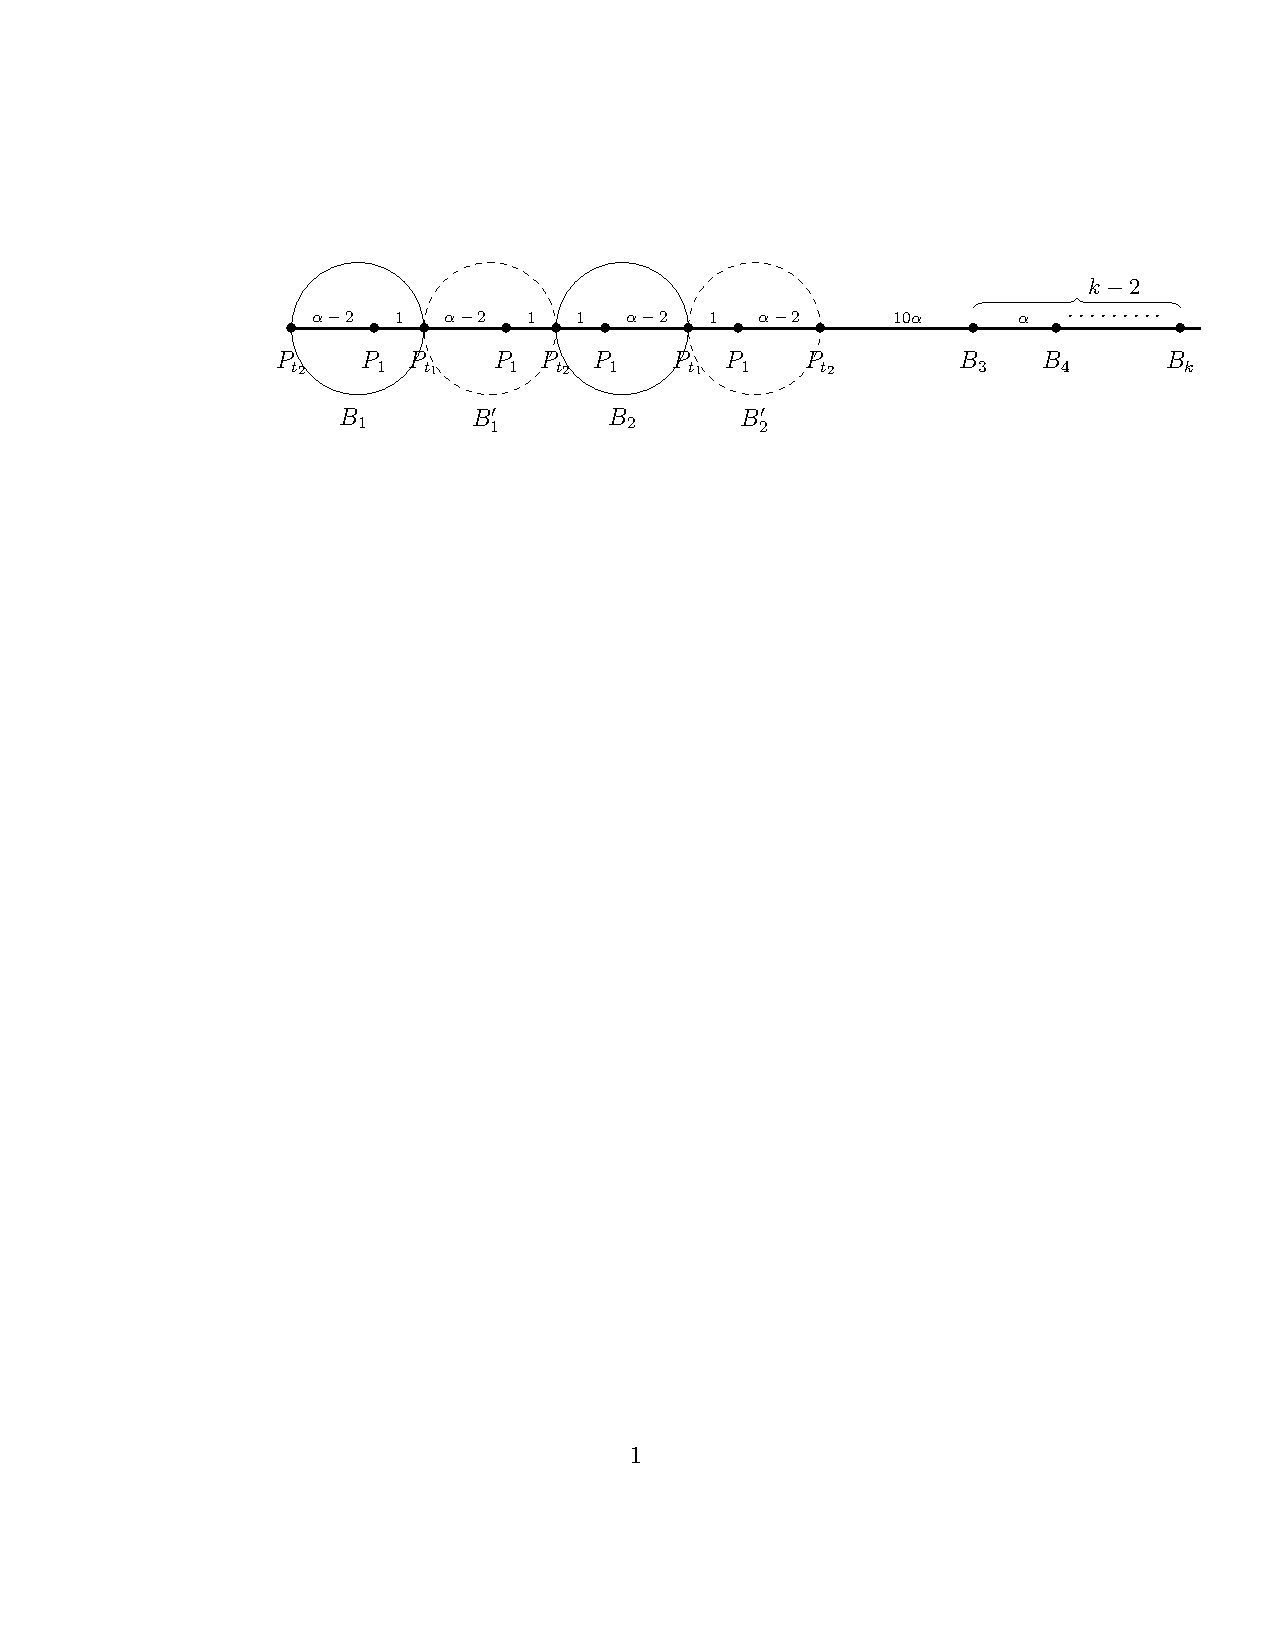
\includegraphics[trim={47mm 205mm 12mm 44mm},clip,width=\textwidth]{figures/clusteringNoise/lbdFig2.pdf}
\end{center}
\vspace{-1cm}
\caption{$\mc X \subseteq \mathbb{R}$ such that no tree can capture all the $(\alpha, \eta)$-proximal clusterings.}
\label{fig:noalgalphacp}
\end{figure}

\noindent\textbf{Proof of Theorem~\ref{thm:nolistalphacp}}
The clustering instance $\mc X$ is an extension of Fig. \ref{fig:noalgalphacp}. Let  $G_1 = \{B_1, B_1', B_2, B_2'\}$ be the balls as in Fig. \ref{fig:noalgalphacp}. Now, construct $G_2 = \{B_3, B_3', B_4, B_4'\}$ exactly identical to $G_1$ but far. In this way, we construct $k/2$ copies of $G_1$. \qed\\

\noindent\textbf{Proof of Theorem~\ref{thm:nosparsealg}}
Let $\mc X \subseteq \mathbb{R}$ be as shown in Fig. \ref{fig:nosparsealg}. Let $t' = \frac{t}{2}-1$ and let $B_1, B_2, B_3, B_1'$, $B_2', B_3', B_1'', B_2''$ and $B_3''$ be as shown in Fig.~\ref{fig:nosparsealg}. For $\alpha \le 2\sqrt{2}+3$, clusterings $\mc C_{\mc S} = \{B_1, B_2, B_3, \ldots, B_k\}$, $\mc C_{\mc S'} = \{\ B_1', B_2', B_3, \ldots, B_k\}$ and $\mc C_{\mc S}'' = \{\ B_1'', B_2'', B_3, \ldots, B_k\}$ satisfy $(\alpha, 1)$-center proximity. Also, $m(\mc C_{\mc S}) = m(\mc C_{\mc S}') =$ $m(\mc C_{\mc S}'') = t$. Arguing similarly as in Theorem \ref{thm:noalgalphacp} completes the proof. \qed\\
\begin{figure}[!t]
\vspace{-5mm}
\begin{center}
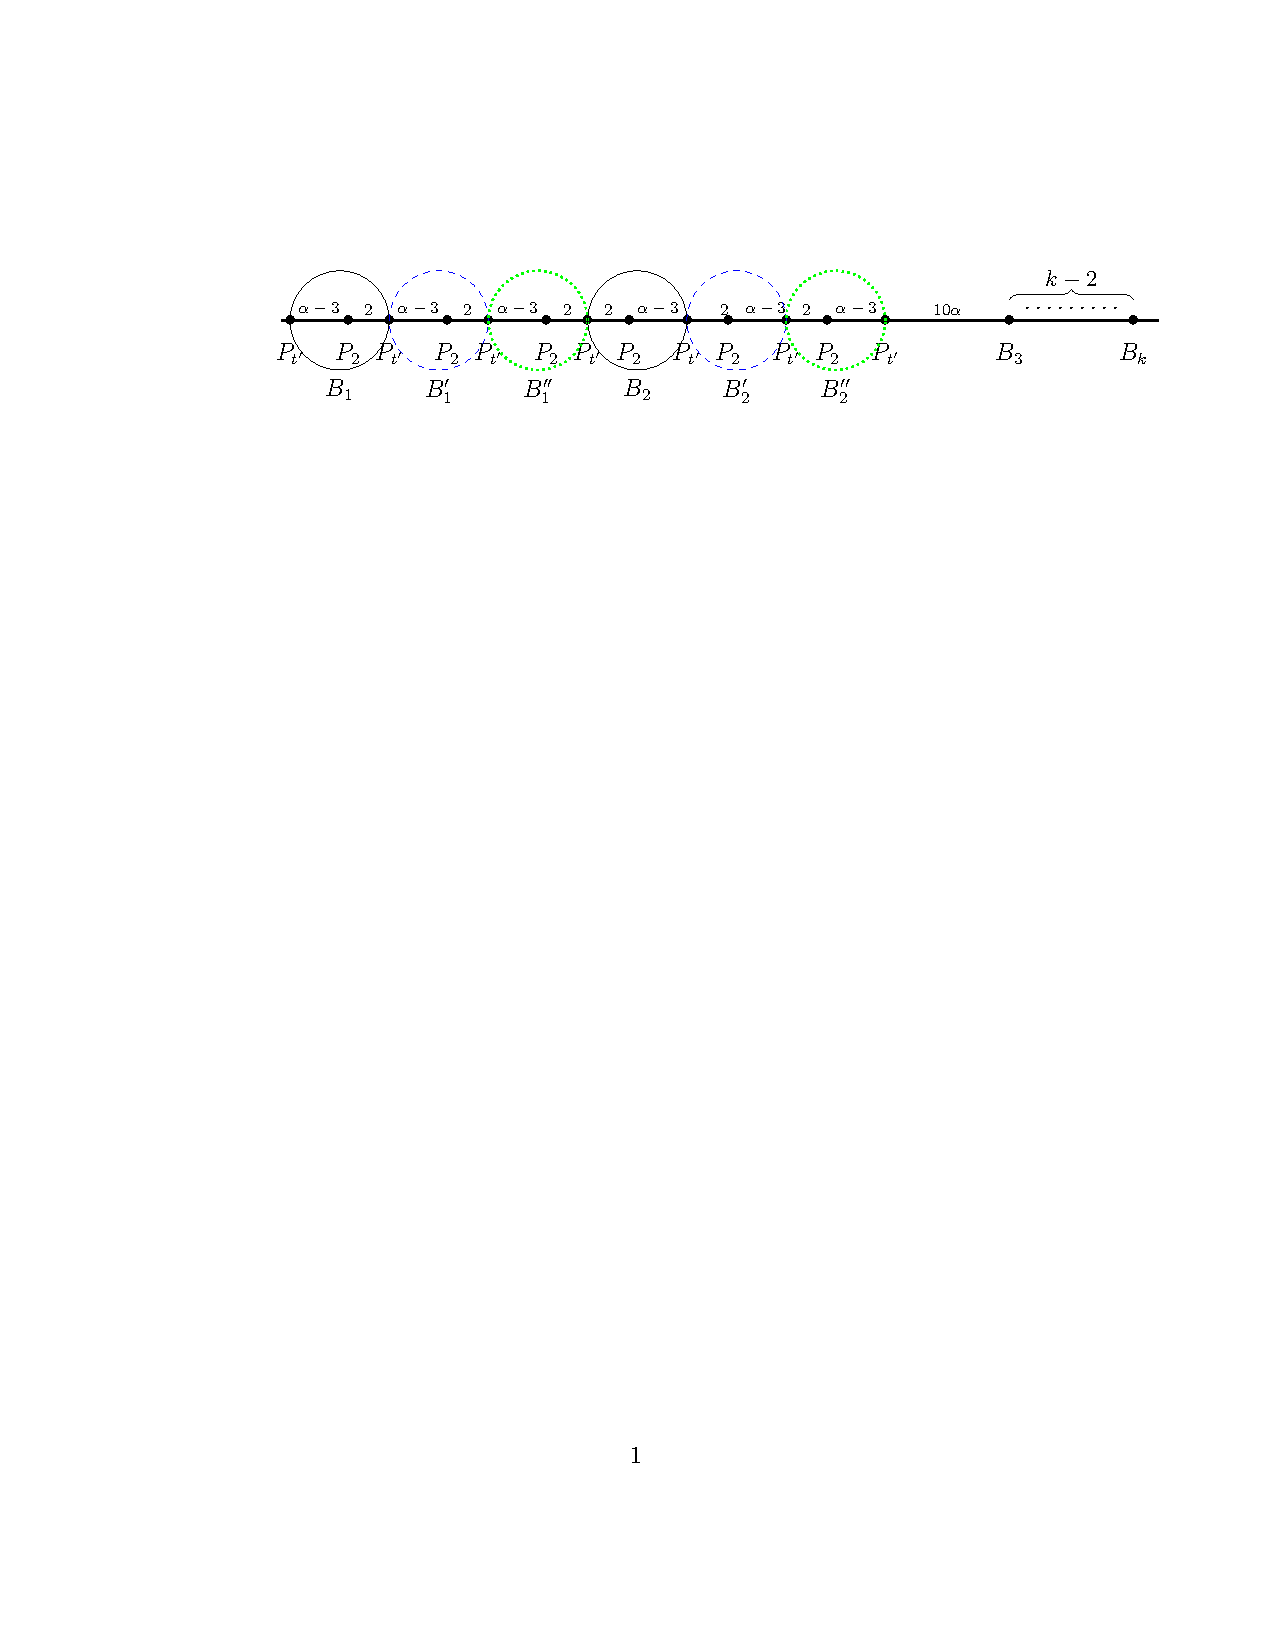
\includegraphics[trim={45mm 210mm 20mm 43mm},clip,width=\textwidth]{figures/clusteringNoise/lbdFig3.pdf}
\end{center}
\vspace{-4mm}
\caption{$\mc X \subseteq \mathbb{R}$ such that no algorithm can capture all the $\alpha$-proximal clusterings. } 
\label{fig:nosparsealg}
\end{figure}

\noindent\textbf{Proofs of Theorems~\ref{thm:nosparselistalphacp}, \ref{thm:nosparselistlambdacs} and \ref{thm:nolistlambdacs}} have the exact same ideas as the proof of Theorem~\ref{thm:nolistalphacp}. To prove the lower bound in the list model, instance constructed in Theorem~\ref{thm:nolistalphacp} is a simple extension of the instance in Theorem~\ref{thm:noalgalphacp}. The instances for the proof of Theorems~\ref{thm:nosparselistalphacp}, \ref{thm:nosparselistlambdacs} and \ref{thm:nolistlambdacs} are similarly constructed as extensions of their respective tree lower bound instances (Theorems~\ref{thm:nosparsealg}, \ref{thm:nosparselambdaalg} and \ref{thm:noalglambdacs}).

\noindent\textbf{Proof of Theorem~\ref{thm:lambdaNoNoisePositive}}
We will show that $\mc C_{\mc X}^*$ has strong stability (\cite{balcan2008discriminative}) which will complete the proof (Theorem~8 in \cite{balcan2008discriminative}). Let $A \subset C_i^*$ and $B \subseteq C_j^*$. Let $p \in A$ and $q \in C_i^* \setminus A$ be points which achieve the minimum distance between $A$ and $C_i^*\setminus A$. If $c_i \in A$ then $d(p, q) \le d(c_i, q) \le r$. If $c_i \in C_i^* \setminus A$ then $d(p, q) \le d(p, c_i) \le r$. Hence, $d_{min} (A, C_i^*\setminus A) \le r$. Similarly, we get that $d_{min}(A, B) > r$.\qed\\

\noindent\textbf{Proof of Theorems~\ref{thm:nosparselambdaalg} and \ref{thm:noalglambdacs}} are also identical to the proofs of Theorem~\ref{thm:nosparsealg} and \ref{thm:noalgalphacp}.\\

\noindent\textbf{Proof of Theorem~\ref{thm:lambdacsnoise}}
Fix $\mc S \subseteq \mc X$. Denote by $r_i := r(S_i^*)$. Let $\mc C_{\mc X} = \{C_1, \ldots, \\C_k\}$ be the clustering outputed by the algorithm. Let $\mc L = \{B_1, \ldots, B_l\}$ be the list of balls as outputed by Phase 1 of Alg.~\ref{alg:lambdacs}. Let $G$ be the graph as constructed in Phase 2 of the algorithm. Observe that $B = B(s_i, r_i) = S_i^* \in \mc L$. WLOG, denote this ball by $B^{(i)}$ and the corresponding vertex in the graph $G$ by $v^{(i)}$. We will prove the theorem by proving two key facts.  

\begin{enumerate}[nolistsep,noitemsep,label=\textbf{F.\arabic*},leftmargin=0.3in]
\renewcommand\labelitemi{$\diamond$}
\item \label{fact:lambda1} If $B_{i1}$ and $B_{i2}$ intersect $S_i^*$ then the vertices $v_{i1}$ and $v_{i2}$ are connected.
\item \label{fact:lambda2} If $B_{i1}$ intersects $S_i^*$ and $B_{j1}$ intersects $S_j^*$ then $v_{i1}$ and $v_{j1}$ are disconnected in $G$.	
\end{enumerate}

\vspace{-0.1in}
\begin{smallLemma}
\label{claim:lambda1}
Let $\mc L, G, B^{(i)}$ and $v^{(i)}$ be as defined above. Let balls $B_{i1}, B_{i2} \in \mc L$ be such that $B_{i1} \cap S_i^* \neq \emptyset$ and $B_{i2} \cap S_i^* \neq \emptyset$. Then there exists a path between $v_{i1}$ and $v_{i2}$.
\end{smallLemma}
\vspace{-0.1in} Assume that $v_{i1}$ and $v^{(i)}$ are not connected by an edge. Hence, $|B_{i1} \setminus B^{(i)}| \ge t/2$. Since $\lambda > 4$, for all $j \neq i$, $B_{i1} \cap S_j^* = \emptyset$. Thus, $B_{i1} \setminus B^{(i)} \subseteq \mc X \setminus \mc S$. which contradicts $|B_{i1} \cap \{\mc X \setminus \mc S\}| < t/2$.\qed

%\vspace{-0.1in}
\begin{smallLemma}
Let the framework be as in Claim~\ref{claim:lambda1}. Let $B_{i1} \in \mc L$ be such that $B_{i1} \cap S_i^* \neq \emptyset$ and $B_{j1}$ be such that $B_{j1} \cap S_j^* \neq \emptyset$. Then $v_{i1}$ and $v_{j1}$ are disconnected in $G$.
\end{smallLemma}
\vspace{-0.1in} Assume that $v_{i1}$ and $v_{j1}$ are connected. Hence, there exists vertices $v_{i}$ and $v_{n}$ such that $v_i$ and $v_n$ are connected by an edge in $G$ and $B_i \cap S_i^* \neq \emptyset$ and $B_n \cap S_n^* \neq \emptyset$ for some $n \neq i$. $|B_i \cap B_n| \ge t/2$. Now, $\lambda \ge 4$, thus $B_i \cap \{\mc S \setminus S_i^*\} = \emptyset$ and $B_n \cap \{\mc S\setminus S_n^*\} = \emptyset$. Thus, $B_i \cap B_n \subseteq \mc X \setminus \mc S$ which contradicts the sparseness assumption.
\qed

\label{appendix:sectiontr}
\begin{theorem}[Vapnik and Chervonenkis \cite{vapnik2015uniform}]\label{theorem:vceapprox}
Let $X$ be a domain set and $D$ a probability distribution over $X$. Let $H$ be a class of subsets of $X$ of finite VC-dimension $d$. Let $\epsilon, \delta \in (0,1)$. Let $S \subseteq X$ be picked i.i.d according to $D$ of size $m$. If $m > \frac{c}{\epsilon^2}(d\log \frac{d}{\epsilon}+\log\frac{1}{\delta})$, then  with probability $1-\delta$ over the choice of $S$, we have that $\forall h \in H$
$$\bigg|\frac{|h\cap S|}{|S|} - P(h)\bigg| < \epsilon$$
\end{theorem}

\end{subappendices}

\cleardoublepage 
\phantomsection  

\renewcommand*{\bibname}{References}

\addcontentsline{toc}{chapter}{\textbf{References}}
\bibliography{uw-ethesis}
\bibliographystyle{plain}
%\nocite{*}

\appendix
\chapter*{APPENDICES}
\addcontentsline{toc}{chapter}{APPENDICES}
%======================================================================
\chapter[Technical lemmas]{Technical lemmas}
\label{appendix:technicalLemmas}
\def\COMPLETE{}




\end{document}
\grid
